% !TeX program = xelatex
% MAU DINH DANG BAO CAO TU PDF Assignment_Xac_suat_thong_ke.
% Day la mau bo cuc co the chinh sua, khong phai ban chep toan van PDF.
% Bien dich bang XeLaTeX 2 lan de cap nhat muc luc va tong so trang.
% Dat logo_bach_khoa.png cung thu muc voi tep .tex nay.
\documentclass[10pt,a4paper]{article}

% ==================== 1. TIENG VIET VA PHONG CHU ====================
\usepackage{fontspec}
\setmainfont{Latin Modern Roman}
\setsansfont{Latin Modern Sans}
\setmonofont{Latin Modern Mono}
\usepackage{polyglossia}
\setdefaultlanguage{vietnamese}

% ==================== 2. KHO GIAY VA LE TRANG ======================
% Cac kich thuoc duoc dung lai theo bo cuc quan sat trong PDF mau.
\usepackage[
  a4paper,
  left=3.15cm,right=3.15cm,
  top=4.30cm,bottom=3.90cm,
  headheight=27pt,headsep=15pt,footskip=19pt
]{geometry}
\setlength{\parindent}{15pt}
\setlength{\parskip}{0pt}
\linespread{1}
\raggedbottom
\setlength{\emergencystretch}{1.5em}

% ==================== 3. CAC GOI DINH DANG =========================
\usepackage{amsmath,amssymb,mathtools}
\usepackage{unicode-math}
\setmathfont{Latin Modern Math}
\usepackage{graphicx}
\usepackage[table]{xcolor}
\definecolor{TableHead}{HTML}{E8EDF2}
\usepackage{array,tabularx,longtable,booktabs}
\newcolumntype{L}[1]{>{\raggedright\arraybackslash}p{#1}}
\newcolumntype{C}[1]{>{\centering\arraybackslash}p{#1}}
\providecommand{\tightlist}{\setlength{\itemsep}{0pt}\setlength{\parskip}{0pt}}
\usepackage{float}
\usepackage{caption}
\usepackage{enumitem}
\usepackage{titlesec}
\usepackage{fancyhdr}
\usepackage{lastpage}
\usepackage{listings}
\usepackage{tikz}
\usetikzlibrary{positioning,arrows.meta}
\usepackage{hyperref}
\hypersetup{hidelinks,unicode=true,pdfauthor={},
  pdftitle={Phân tích các yếu tố ảnh hưởng đến công suất tiêu thụ của GPU rời}}
\urlstyle{same}

% ==================== 4. THONG TIN CAN THAY ========================
% Sua cac lenh duoi day de dung cho bai cua nhom.
\newcommand{\TenDaiHoc}{ĐẠI HỌC QUỐC GIA THÀNH PHỐ HỒ CHÍ MINH}
\newcommand{\TenTruong}{TRƯỜNG ĐẠI HỌC BÁCH KHOA}
\newcommand{\TenKhoa}{KHOA KHOA HỌC VÀ KỸ THUẬT MÁY TÍNH}
\newcommand{\TenMonHoc}{XÁC SUẤT VÀ THỐNG KÊ (MT2013)}
\newcommand{\HocKy}{261}
\newcommand{\NamHoc}{2026 - 2027}
\newcommand{\TenDeTai}{Phân tích các yếu tố ảnh hưởng đến\\
  công suất tiêu thụ của GPU rời}
\newcommand{\GiangVien}{Huỳnh Thái Duy Phương}
\newcommand{\LopNhom}{Lớp L11, Nhóm 19}
\newcommand{\DiaDiemNgayThang}{Thành phố Hồ Chí Minh, tháng 11 năm 2026}
\newcommand{\NoiDungChanTrang}{Bài tập lớn môn học Xác suất và Thống kê
  (Học kỳ \HocKy) - Năm học \NamHoc}

% ==================== 4b. NAP SO LIEU SINH TU PYTHON ===============
% Generated by scripts/reports/report_overview.py; do not edit by hand.
\newcommand{\OvwRowsRaw}{3406}
\newcommand{\OvwColsRaw}{34}
\newcommand{\OvwDefaultNumericCols}{7}
\newcommand{\OvwDefaultObjectCols}{27}
\newcommand{\OvwDateValid}{3376}
\newcommand{\OvwDateMin}{23/03/1998}
\newcommand{\OvwDateMax}{30/09/2017}
\newcommand{\OvwDateUnknown}{30}
\newcommand{\OvwDateUnknownPct}{0,88}
\newcommand{\OvwCoreSpeedDash}{907}
\newcommand{\OvwCoreSpeedBlank}{29}
\newcommand{\OvwCoreSpeedMissing}{936}
\newcommand{\OvwCoreSpeedMissingPct}{27,48}
\newcommand{\OvwManufacturerLevels}{4}
\newcommand{\OvwNvidiaCount}{1743}
\newcommand{\OvwNvidiaPct}{51,17}
\newcommand{\OvwAmdCount}{1317}
\newcommand{\OvwAmdPct}{38,67}
\newcommand{\OvwIntelCount}{254}
\newcommand{\OvwIntelPct}{7,46}
\newcommand{\OvwAtiCount}{92}
\newcommand{\OvwAtiPct}{2,70}
\newcommand{\OvwDedicatedYes}{3018}
\newcommand{\OvwDedicatedNo}{374}
\newcommand{\OvwDedicatedMissing}{14}
\newcommand{\OvwNotebookYes}{709}
\newcommand{\OvwNotebookNo}{2697}
\newcommand{\OvwPowerObserved}{2781}
\newcommand{\OvwPowerMissing}{625}
\newcommand{\OvwPowerMissingPct}{18,35}
\newcommand{\OvwPriceMissingPct}{83,68}
\newcommand{\OvwDpMissingPct}{74,84}
\newcommand{\OvwBoostMissingPct}{57,55}

% Generated by scripts/reports/report_preprocessing.py; do not edit by hand.
\newcommand{\PreRowsRaw}{3406}
\newcommand{\PreColsRaw}{34}
\newcommand{\PreColsSelected}{18}
\newcommand{\PreCellsMarkedMissing}{6474}
\newcommand{\PreReleaseYearMin}{2003}
\newcommand{\PreReleaseYearMax}{2017}
\newcommand{\PreCoreSpeedDash}{907}
\newcommand{\PreCoreSpeedBlank}{29}
\newcommand{\PreUnknownReleaseDate}{30}
\newcommand{\PreBandwidthInMb}{4}
\newcommand{\PreRopsMultiplier}{305}
\newcommand{\PreTextureUntestable}{31}
\newcommand{\PreBandwidthMismatchNotRepaired}{7}
\newcommand{\PreBandwidthMismatchShifted}{3}
\newcommand{\PreTextureMismatchBefore}{274}
\newcommand{\PreTextureMismatchAfter}{0}
\newcommand{\PreBandwidthMismatchBefore}{312}
\newcommand{\PreBandwidthMismatchAfter}{4}
\newcommand{\PreEncodingFixed}{1}
\newcommand{\PreRepairedYears}{2016--2017}
\newcommand{\PreRepairedInFinal}{100}
\newcommand{\PreNotebookYes}{709}
\newcommand{\PreNotebookNo}{2697}
\newcommand{\PreManufacturerLevels}{4}
\newcommand{\PreManufacturerNames}{Nvidia, AMD, Intel, ATI}
\newcommand{\PreMemoryTypeLevels}{12}
\newcommand{\PreMemoryTypeMissing}{56}
\newcommand{\PreMemoryTypeLevelsFinal}{10}
\newcommand{\PreMemoryTypeGroups}{6}
\newcommand{\PreMemoryTypeOtherNames}{DDR, GDDR2, GDDR4, HBM-1, HBM-2}
\newcommand{\PreIntegrated}{374}
\newcommand{\PreUnknownDedicated}{14}
\newcommand{\PreRowsDedicated}{3018}
\newcommand{\PreRowsSingleGpu}{2775}
\newcommand{\PreRowsReleased}{2762}
\newcommand{\PreRowsScoped}{2762}
\newcommand{\PreRowsFinal}{2057}
\newcommand{\PreIncompleteRemoved}{705}
\newcommand{\PreIntelFinal}{0}
\newcommand{\PreMultiGpuRemoved}{243}
\newcommand{\PreUnreleasedRemoved}{13}
\newcommand{\PreDuplicatesRemoved}{0}
\newcommand{\PreLaptopAuxPower}{37}
\newcommand{\PreColsFinal}{16}
\newcommand{\PreDesktop}{1786}
\newcommand{\PreLaptop}{271}
\newcommand{\PreInvalidPowerRows}{1}
\newcommand{\PreInvalidPowerSiblings}{2}
\newcommand{\PreInvalidPowerSiblingWatts}{127}
\newcommand{\PrePowerMissing}{482}
\newcommand{\PrePowerMissingPct}{17,5}
\newcommand{\PreMissingMeanYear}{2009,0}
\newcommand{\PreObservedMeanYear}{2012,7}
\newcommand{\PreMissingYearZ}{-19{,}20}
\newcommand{\PreMissingYearP}{$<$ 0,001}
\newcommand{\PreMissingAmdPct}{53,2}
\newcommand{\PreObservedAmdPct}{38,9}
\newcommand{\PreMissingMakerZ}{5{,}71}
\newcommand{\PreMissingMakerP}{$<$ 0,001}
\newcommand{\PreAtiCards}{83}
\newcommand{\PreAtiMissing}{0}
\newcommand{\PreIntelCards}{7}
\newcommand{\PreLostPowerMean}{63,8}
\newcommand{\PreLostPowerZ}{-14{,}31}
\newcommand{\PreLostPowerP}{$<$ 0,001}
\newcommand{\PreLostMeanYear}{2008,0}
\newcommand{\PreKeptMeanYear}{2013,1}
\newcommand{\PreFinalPowerMean}{124,9}
\newcommand{\PreFinalPowerMedian}{120}
\newcommand{\PreAllPowerMean}{119,0}
\newcommand{\PreAllPowerMedian}{110}
\newcommand{\PreFinalDesktopAuxPct}{71,1}
\newcommand{\PreAllDesktopAuxPct}{68,5}
\newcommand{\PreUnknownYearRows}{30}
\newcommand{\PreUnknownYearPowerMissingPct}{6,7}
\newcommand{\PreUnknownYearDroppedPct}{100,0}
\newcommand{\PreCoreExplainedPct}{60}
\newcommand{\PreCoreMissingInFinal}{220}
\newcommand{\PreCoreMissingInFinalPct}{10,7}
\newcommand{\PreCoreKnownInFinal}{1837}
\newcommand{\PreRowsIfCoreRequired}{1837}
\newcommand{\PreCoreProcessCorr}{-0{,}74}
\newcommand{\PreCoreYearCorr}{0{,}75}
\newcommand{\PreCoreWithinChipSpreadPct}{6}
\newcommand{\PreCoreBetweenChipSpreadPct}{26}
\newcommand{\PreCoreWithinChipElasticity}{0,5}
\newcommand{\PreCoreWithinChipCards}{1627}
\newcommand{\PreCoreWithinChipChips}{132}
\newcommand{\PreCoreMissingPowerMean}{99,7}
\newcommand{\PreCoreKnownPowerMean}{127,9}
\newcommand{\PreNvidiaFinalMean}{126,7}
\newcommand{\PreNvidiaAllMean}{118,7}
\newcommand{\PreNvidiaMinusAmdFinal}{4{,}1}
\newcommand{\PreNvidiaMinusAmdAll}{-0{,}4}
\newcommand{\PreMemoryTypeOtherSize}{18}
\newcommand{\PrePowerFarFromChipMedian}{11}
\newcommand{\PreLowPowerLaptopCards}{11}
\newcommand{\PreRowsBeforeTwoThousandSix}{7}
\newcommand{\PreRowsWithPower}{2280}
\newcommand{\PreRowsIncomplete}{705}
\newcommand{\PreRowsIncompletePct}{25,5}
\newcommand{\PrePowerRowsLostByDropAll}{223}
\newcommand{\PrePowerMeanDropped}{119,0}
\newcommand{\PrePowerMeanImputed}{117,4}
\newcommand{\PrePowerSdDropped}{77,5}
\newcommand{\PrePowerSdImputed}{70,5}
\newcommand{\PrePowerCiDropped}{3,2}
\newcommand{\PrePowerCiImputed}{2,6}
\newcommand{\PrePowerAtMedianDropped}{1,0}
\newcommand{\PrePowerAtMedianImputed}{18,3}
\newcommand{\PreMissingPctGpuId}{0,0}
\newcommand{\PreMissingPctName}{0,0}
\newcommand{\PreMissingPctManufacturer}{0,0}
\newcommand{\PreMissingPctSegment}{0,0}
\newcommand{\PreMissingPctMemoryType}{0,7}
\newcommand{\PreMissingPctMemoryTypeGroup}{0,7}
\newcommand{\PreMissingPctArchitecture}{1,5}
\newcommand{\PreMissingPctReleaseYear}{1,1}
\newcommand{\PreMissingPctMaxPowerW}{17,5}
\newcommand{\PreMissingPctNeedsAuxPower}{17,5}
\newcommand{\PreMissingPctTextureRatePerWatt}{24,2}
\newcommand{\PreMissingPctTmus}{13,0}
\newcommand{\PreMissingPctMemoryBandwidthGbS}{1,3}
\newcommand{\PreMissingPctMemoryMb}{0,9}
\newcommand{\PreMissingPctProcessNm}{10,5}
\newcommand{\PreMissingPctCoreSpeedMhz}{22,0}

% Generated by scripts/reports/report_anova.py; do not edit by hand.
\newcommand{\AnovaRows}{2039}
\newcommand{\AnovaGroups}{5}
\newcommand{\AnovaOtherRows}{18}
\newcommand{\AnovaDfBetween}{4}
\newcommand{\AnovaDfWithin}{2034}
\newcommand{\AnovaSsBetween}{4\,091\,827}
\newcommand{\AnovaSsWithin}{7\,807\,607}
\newcommand{\AnovaSsTotal}{11\,899\,434}
\newcommand{\AnovaMsBetween}{1\,022\,957}
\newcommand{\AnovaMsWithin}{3\,839}
\newcommand{\AnovaClassicF}{266{,}50}
\newcommand{\AnovaClassicFCritical}{2{,}38}
\newcommand{\AnovaClassicP}{2{,}7 \cdot 10^{-184}}
\newcommand{\AnovaEtaSq}{0{,}344}
\newcommand{\AnovaEtaSqPercent}{34{,}4}
\newcommand{\AnovaWelchF}{1214{,}96}
\newcommand{\AnovaWelchDfOne}{4}
\newcommand{\AnovaWelchDfTwo}{170{,}6}
\newcommand{\AnovaWelchFCritical}{2{,}42}
\newcommand{\AnovaWelchP}{3{,}7 \cdot 10^{-124}}
\newcommand{\AnovaLeveneW}{88{,}96}
\newcommand{\AnovaLeveneP}{9{,}5 \cdot 10^{-70}}
\newcommand{\AnovaSdRatio}{4{,}1}
\newcommand{\AnovaSdMaxGroup}{GDDR5}
\newcommand{\AnovaSdMinGroup}{DDR2}
\newcommand{\AnovaSizeMin}{33}
\newcommand{\AnovaSizeMinGroup}{DDR2}
\newcommand{\AnovaSizeMax}{1488}
\newcommand{\AnovaSizeOtherMin}{76}
\newcommand{\AnovaDdrThreeLaptopPercent}{40}
\newcommand{\AnovaGddrFiveXLevels}{180, 220, 250}
\newcommand{\AnovaGddrFiveXLevelCards}{71}
\newcommand{\AnovaGddrFiveXCards}{76}
\newcommand{\AnovaArchLabels}{347}
\newcommand{\AnovaGddrThreeKept}{117}
\newcommand{\AnovaGddrThreeWithPower}{230}
\newcommand{\AnovaGddrThreeMeanKept}{80{,}6}
\newcommand{\AnovaGddrThreeMeanAll}{67{,}8}
\newcommand{\AnovaGddrFiveXArchLabels}{3}
\newcommand{\AnovaGddrFiveXMinusGddrFive}{68}
\newcommand{\AnovaGddrFiveXMinusGddrFiveLow}{48{,}2}
\newcommand{\AnovaGddrFiveXMinusGddrFiveHigh}{88{,}0}
\newcommand{\AnovaDdrThreeMinusDdrTwoLow}{-28{,}5}
\newcommand{\AnovaDdrThreeMinusDdrTwoHigh}{33{,}3}
\newcommand{\AnovaDdrThreeMinusDdrTwoGamesLow}{-6{,}6}
\newcommand{\AnovaDdrThreeMinusDdrTwoGamesHigh}{11{,}5}
\newcommand{\AnovaKruskalH}{833{,}6}
\newcommand{\AnovaKruskalP}{4{,}0 \cdot 10^{-179}}
\newcommand{\AnovaPairs}{10}
\newcommand{\AnovaPairsSignificant}{9}
\newcommand{\AnovaPairsNotSignificant}{DDR3--DDR2}
\newcommand{\AnovaGamesSignificant}{9}
\newcommand{\AnovaGamesNotSignificant}{DDR3--DDR2}

% Generated by scripts/reports/report_anova_two_way.py; do not edit by hand.
\newcommand{\AnovaAlpha}{0{,}05}
\newcommand{\AnovaTotalCleaned}{2057}
\newcommand{\AnovaAtiDesktop}{77}
\newcommand{\AnovaAtiLaptop}{0}
\newcommand{\AnovaSampleN}{1980}
\newcommand{\AnovaDfErr}{1976}
\newcommand{\AnovaFCrit}{3{,}846}
\newcommand{\AnovaTCrit}{1{,}9612}
\newcommand{\AnovaCellAmdDesktopN}{677}
\newcommand{\AnovaCellAmdLaptopN}{117}
\newcommand{\AnovaCellNvidiaDesktopN}{1032}
\newcommand{\AnovaCellNvidiaLaptopN}{154}
\newcommand{\AnovaRawAmdDesktopMean}{137{,}28}
\newcommand{\AnovaRawAmdLaptopMean}{37{,}03}
\newcommand{\AnovaRawNvidiaDesktopMean}{138{,}06}
\newcommand{\AnovaRawNvidiaLaptopMean}{50{,}18}
\newcommand{\AnovaRawLaptopGapW}{13{,}15}
\newcommand{\AnovaRawAmdDesktopSd}{83{,}76}
\newcommand{\AnovaRawAmdLaptopSd}{28{,}26}
\newcommand{\AnovaRawLeveneW}{76{,}964}
\newcommand{\AnovaRawLeveneP}{$<$ 0{,}001}
\newcommand{\AnovaRawSdRatio}{2{,}96}
\newcommand{\AnovaRawShapiroW}{0{,}9707}
\newcommand{\AnovaRawShapiroP}{$<$ 0{,}001}
\newcommand{\AnovaRawMsErr}{5\,089{,}8}
\newcommand{\AnovaRawFMaker}{2{,}181}
\newcommand{\AnovaRawPMaker}{$=$ 0{,}1399}
\newcommand{\AnovaRawEtaMaker}{0{,}0011}
\newcommand{\AnovaRawFSeg}{397{,}709}
\newcommand{\AnovaRawPSeg}{$<$ 0{,}001}
\newcommand{\AnovaRawEtaSeg}{0{,}1675}
\newcommand{\AnovaRawEtaSegPct}{16{,}8}
\newcommand{\AnovaRawFInter}{1{,}718}
\newcommand{\AnovaRawPInter}{$=$ 0{,}1901}
\newcommand{\AnovaRawEtaInter}{0{,}0009}
\newcommand{\AnovaRawTukeyMinDeskLapW}{87{,}10}
\newcommand{\AnovaRawTukeyMaxDeskLapW}{101{,}04}
\newcommand{\AnovaRawWelchLaptopT}{-3{,}341}
\newcommand{\AnovaRawWelchLaptopP}{$<$ 0{,}001}
\newcommand{\AnovaRawWelchDesktopP}{$=$ 0{,}8401}
\newcommand{\AnovaLogLeveneW}{11{,}558}
\newcommand{\AnovaLogLeveneP}{$<$ 0{,}001}
\newcommand{\AnovaLogSdRatio}{1{,}23}
\newcommand{\AnovaLogShapiroW}{0{,}9622}
\newcommand{\AnovaLogShapiroP}{$<$ 0{,}001}
\newcommand{\AnovaLogAmdLapShapiroW}{0{,}9795}
\newcommand{\AnovaLogAmdLapShapiroP}{$=$ 0{,}0701}
\newcommand{\AnovaLogFMaker}{22{,}537}
\newcommand{\AnovaLogPMaker}{$<$ 0{,}001}
\newcommand{\AnovaLogEtaMaker}{0{,}0113}
\newcommand{\AnovaLogFSeg}{725{,}710}
\newcommand{\AnovaLogPSeg}{$<$ 0{,}001}
\newcommand{\AnovaLogEtaSeg}{0{,}2686}
\newcommand{\AnovaLogEtaSegPct}{26{,}9}
\newcommand{\AnovaLogFInter}{8{,}767}
\newcommand{\AnovaLogPInter}{$=$ 0{,}0031}
\newcommand{\AnovaLogEtaInter}{0{,}0044}
\newcommand{\AnovaGeomAmdDesktop}{108{,}4}
\newcommand{\AnovaGeomNvidiaDesktop}{117{,}5}
\newcommand{\AnovaGeomAmdLaptop}{28{,}2}
\newcommand{\AnovaGeomNvidiaLaptop}{39{,}9}
\newcommand{\AnovaLaptopGeomGapPct}{41{,}5}
\newcommand{\AnovaDesktopGeomGapPct}{8{,}4}
\newcommand{\AnovaLogTukeyDeskP}{$=$ 0{,}0796}
\newcommand{\AnovaLogTukeyLapP}{$<$ 0{,}001}
\newcommand{\AnovaLogMsErr}{0{,}4646}
\newcommand{\AnovaRawLsdSigCount}{4}
\newcommand{\AnovaLogLsdSigCount}{6}
\newcommand{\AnovaLogLsdDeskDiff}{0{,}0805}
\newcommand{\AnovaLogLsdDeskCrit}{0{,}0661}
\newcommand{\AnovaLogLsdLapDiff}{0{,}3474}
\newcommand{\AnovaLogLsdLapCrit}{0{,}1639}
\newcommand{\AnovaLogWelchDesktopP}{$=$ 0{,}0212}
\newcommand{\AnovaLogWelchLaptopP}{$<$ 0{,}001}

% Generated by scripts/reports/report_regression.py; do not edit.
\newcommand{\RegN}{1837}
\newcommand{\RegRowsExcluded}{220}
\newcommand{\RegRowsInput}{2057}
\newcommand{\RegClusters}{273}
\newcommand{\RegAlpha}{0{,}005}
\newcommand{\RegConfidence}{99{,}5}
\newcommand{\RegRSquared}{0{,}8795}
\newcommand{\RegAdjRSquared}{0{,}8790}
\newcommand{\RegPrimaryF}{273{,}505}
\newcommand{\RegPrimaryP}{\ensuremath{5{,}25 \cdot 10^{-94}}}
\newcommand{\RegPrimaryDfOne}{4}
\newcommand{\RegPrimaryDfTwo}{272}
\newcommand{\RegMaxVIF}{4{,}123}
\newcommand{\RegCVRMSE}{31{,}56}
\newcommand{\RegCVMAE}{22{,}70}
\newcommand{\RegCVRSquaredW}{0{,}8364}
\newcommand{\RegReject}{1}


% ==================== 5. DAU TRANG VA CHAN TRANG ===================
\newcommand{\LogoTruong}[1]{%
  \IfFileExists{logo_bach_khoa.png}{%
    
\includegraphics[width=#1]{logo_bach_khoa.png}%
  }{\fbox{\parbox[c][#1][c]{#1}{\centering\scriptsize LOGO}}}%
}
\pagestyle{fancy}
\fancyhf{}
\fancyhead[L]{%
  \begin{minipage}[c]{1.5cm}
    \hspace*{2mm}\LogoTruong{8mm}
  \end{minipage}%
  \begin{minipage}[c]{\dimexpr\textwidth-1.5cm\relax}
    \ttfamily\fontsize{10}{12}\selectfont
    Trường Đại học Bách khoa TP. Hồ Chí Minh\\
    Khoa Khoa học và Kỹ thuật Máy tính
  \end{minipage}%
}
\fancyfoot[L]{\ttfamily\fontsize{7}{9}\selectfont\NoiDungChanTrang}
\fancyfoot[R]{\ttfamily\fontsize{7}{9}\selectfont Page \thepage/\pageref*{LastPage}}
\renewcommand{\headrulewidth}{0.4pt}
\renewcommand{\footrulewidth}{0.4pt}
\fancypagestyle{plain}{\pagestyle{fancy}}

% ==================== 6. TIEU DE VA MUC LUC ========================
\setcounter{secnumdepth}{4}
\setcounter{tocdepth}{4}
\titleformat{\section}{\normalfont\Large\bfseries}{\thesection}{1em}{}
\titleformat{\subsection}{\normalfont\large\bfseries}{\thesubsection}{1em}{}
\titleformat{\subsubsection}{\normalfont\normalsize\bfseries}{\thesubsubsection}{1em}{}
% Cap thu tu theo mau: 5.1.2.a, 5.1.2.b, ...
\renewcommand{\theparagraph}{\thesubsubsection.\alph{paragraph}}
\titleformat{\paragraph}[block]{\normalfont\normalsize\bfseries}{\theparagraph}{1em}{}
\titlespacing*{\section}{0pt}{3.5ex plus 1ex minus .2ex}{2.3ex plus .2ex}
\titlespacing*{\subsection}{0pt}{3.25ex plus 1ex minus .2ex}{1.5ex plus .2ex}
\titlespacing*{\subsubsection}{0pt}{3.25ex plus 1ex minus .2ex}{1.5ex plus .2ex}
\titlespacing*{\paragraph}{0pt}{2ex plus .5ex}{1ex}
\setlist[itemize]{leftmargin=2.5em,itemsep=.7ex,topsep=.8ex}
\setlist[enumerate]{leftmargin=2.5em,itemsep=.7ex,topsep=.8ex}
\gappto\captionsvietnamese{%
  \renewcommand{\contentsname}{Mục lục}%
  \renewcommand{\listfigurename}{Danh sách hình vẽ}%
  \renewcommand{\listtablename}{Danh sách bảng}%
  \renewcommand{\figurename}{Hình}%
  \renewcommand{\tablename}{Bảng}%
  \renewcommand{\lstlistingname}{Đoạn code}%
  \renewcommand{\refname}{Tài liệu tham khảo}%
}
\captionsetup{font=normalsize,labelfont=normalfont,labelsep=colon,skip=8pt}

% ==================== 7. MA NGUON VA HINH MINH HOA ================
% Mac dinh Python. Co the doi language=R neu can trinh bay ma R.
\definecolor{codegreen}{RGB}{0,110,0}
\definecolor{codeblue}{RGB}{0,0,160}
\lstdefinestyle{maubaocao}{%
  language=Python,
  basicstyle=\ttfamily\footnotesize,
  keywordstyle=\color{codeblue},
  commentstyle=\color{codegreen},
  stringstyle=\color{codegreen},
  showstringspaces=false,
  keepspaces=true,
  columns=fullflexible,
  breaklines=true,
  breakatwhitespace=false,
  tabsize=4,
  frame=none,
  numbers=none,
  aboveskip=6pt,belowskip=6pt
}
\lstset{style=maubaocao}
% Chen hinh: \HinhBaoCao{duong_dan_anh}{Chu thich}{nhan-tham-chieu}
% Neu chua co anh, mau tu hien khung trong de van bien dich duoc.
\newcommand{\HinhBaoCao}[3]{%
  \begin{figure}[H]
    \centering
    \IfFileExists{#1}{%
      \includegraphics[width=.96\linewidth,height=.33\textheight,keepaspectratio]{#1}%
    }{%
      \fbox{\begin{minipage}[c][4cm][c]{.92\linewidth}
        \centering\itshape Vị trí chèn hình minh họa\\[6pt]
        \normalfont\small Thay bằng hình hoặc biểu đồ của nhóm.
      \end{minipage}}%
    }
    \caption{#2}\label{#3}
  \end{figure}%
}

\begin{document}

% ==================== TRANG BIA ==================================
% Bia khong danh so. Cac node dat theo vi tri cua PDF tham chieu.
\begin{titlepage}
\thispagestyle{empty}
\begin{tikzpicture}[remember picture,overlay]
  \node[anchor=north,inner sep=0,align=center]
    at ([yshift=-46.7mm]current page.north) {%
      \begin{minipage}{16cm}\centering
        \fontsize{10}{14}\selectfont
        \TenDaiHoc\\\TenTruong\\\TenKhoa
      \end{minipage}};
  \node[anchor=north,inner sep=0]
    at ([yshift=-77.7mm]current page.north) {\LogoTruong{40mm}};
  \node[anchor=north west,inner sep=0]
    at ([xshift=48.2mm,yshift=-141.8mm]current page.north west) {%
      \begin{minipage}{114mm}
        {\fontsize{14.4}{17.3}\selectfont\bfseries\TenMonHoc\par}
        \vspace{5mm}\hrule height .4pt\vspace{4mm}
        {\fontsize{14.4}{17.3}\selectfont\bfseries
          Báo cáo bài tập lớn (Học kỳ 261)\par}
        \vspace{4mm}
        {\fontsize{17.2}{19.3}\selectfont\bfseries Phân tích các yếu tố ảnh hưởng đến công suất tiêu thụ của GPU rời\par}
        \vspace{1mm}\hrule height .4pt
      \end{minipage}};
  \node[anchor=north west,inner sep=0]
    at ([xshift=56mm,yshift=-197.8mm]current page.north west) {%
      \begin{minipage}{139mm}
        \fontsize{10}{12.4}\selectfont
        \begin{tabular}{@{}r@{\hspace{4mm}}l@{}}
          Giảng viên hướng dẫn: & Huỳnh Thái Duy Phương\\[4mm]
          Danh sách thành viên: & [Nguyễn Hoàng	Phúc] - [2633036] (Lớp L11, Nhóm 19)\\
          & [Nguyễn Quốc Đạt] - [2510287] (Lớp L11, Nhóm 19)\\
          & [Nguyễn Thái Sơn] - [2510216] (Lớp L11, Nhóm 19)\\
          & [Nguyễn Thanh Lộc] - [2311958] (Lớp L11, Nhóm 19)\\
          & [Văn Đức Hàng] - [2510303] (Lớp L11, Nhóm 19)\\
        \end{tabular}
      \end{minipage}};
  \node[anchor=north,inner sep=0]
    at ([yshift=-236.2mm]current page.north) {%
      \fontsize{8}{10}\selectfont Thành phố Hồ Chí Minh, tháng 11 năm 2026};
\end{tikzpicture}
\null
\end{titlepage}

% ==================== PHAN CONG NHIEM VU ==========================
\pagenumbering{arabic}
\setcounter{page}{1}
\begin{center}
  {\Large\bfseries Bảng phân công nhiệm vụ và mức độ đóng góp\par}
\end{center}
\vspace{3mm}
\begingroup
\setlength{\tabcolsep}{3pt}
\renewcommand{\arraystretch}{1.15}
\noindent\begin{tabularx}{\textwidth}{|c|>{\centering\arraybackslash}p{2.8cm}|c|>{\centering\arraybackslash}X|c|}
  \hline
  \textbf{STT} & \textbf{Họ và tên} & \textbf{MSSV} & \textbf{Nhiệm vụ} & \textbf{Mức độ đóng góp}\\\hline
  1 & [Nguyễn Hoàng	Phúc] & [2633036] & [Nhiệm vụ thành viên 1] & [\ldots]\,\%\\\hline
  2 & [Nguyễn Quốc Đạt] & [2510287] & [Nhiệm vụ thành viên 2] & [\ldots]\,\%\\\hline
  3 & [Nguyễn Thái Sơn] & [2510216] & [Nhiệm vụ thành viên 3] & [\ldots]\,\%\\\hline
  4 & [Nguyễn Thanh Lộc] & [2311958] & [Nhiệm vụ thành viên 4] & [\ldots]\,\%\\\hline
  5 & [Văn Đức Hàng] & [2510303] & [Nhiệm vụ thành viên 5] & [\ldots]\,\%\\\hline
\end{tabularx}
\endgroup

% ==================== MUC LUC VA DANH SACH HINH ===================
\clearpage
\tableofcontents
\clearpage
\phantomsection
\addcontentsline{toc}{section}{\listfigurename}
\listoffigures
% Neu can danh sach bang, bo dau % o ba dong sau:
% \clearpage
% \addcontentsline{toc}{section}{\listtablename}
% \listoftables

% ==================== NOI DUNG BAO CAO ============================
\clearpage
\emergencystretch=3em

% Mục 1: Tổng quan dữ liệu
% =====================================================================
% Mục 1. Tổng quan dữ liệu
%
% Gói cần có trong file chính: booktabs, longtable, array, caption, url (hoặc hyperref).
% Trước khi \input file này, file chính phải nạp các con số do code sinh ra:
%   % Generated by scripts/reports/report_overview.py; do not edit by hand.
\newcommand{\OvwRowsRaw}{3406}
\newcommand{\OvwColsRaw}{34}
\newcommand{\OvwDefaultNumericCols}{7}
\newcommand{\OvwDefaultObjectCols}{27}
\newcommand{\OvwDateValid}{3376}
\newcommand{\OvwDateMin}{23/03/1998}
\newcommand{\OvwDateMax}{30/09/2017}
\newcommand{\OvwDateUnknown}{30}
\newcommand{\OvwDateUnknownPct}{0,88}
\newcommand{\OvwCoreSpeedDash}{907}
\newcommand{\OvwCoreSpeedBlank}{29}
\newcommand{\OvwCoreSpeedMissing}{936}
\newcommand{\OvwCoreSpeedMissingPct}{27,48}
\newcommand{\OvwManufacturerLevels}{4}
\newcommand{\OvwNvidiaCount}{1743}
\newcommand{\OvwNvidiaPct}{51,17}
\newcommand{\OvwAmdCount}{1317}
\newcommand{\OvwAmdPct}{38,67}
\newcommand{\OvwIntelCount}{254}
\newcommand{\OvwIntelPct}{7,46}
\newcommand{\OvwAtiCount}{92}
\newcommand{\OvwAtiPct}{2,70}
\newcommand{\OvwDedicatedYes}{3018}
\newcommand{\OvwDedicatedNo}{374}
\newcommand{\OvwDedicatedMissing}{14}
\newcommand{\OvwNotebookYes}{709}
\newcommand{\OvwNotebookNo}{2697}
\newcommand{\OvwPowerObserved}{2781}
\newcommand{\OvwPowerMissing}{625}
\newcommand{\OvwPowerMissingPct}{18,35}
\newcommand{\OvwPriceMissingPct}{83,68}
\newcommand{\OvwDpMissingPct}{74,84}
\newcommand{\OvwBoostMissingPct}{57,55}

% (tạo bằng: python scripts/reports/report_overview.py; script này cũng sinh
% generated/overview_variables_rows.tex cho bảng danh sách 34 biến). Mọi con số
% trong lời văn đều là macro \Ovw..., nên chạy lại code là báo cáo tự cập nhật.
% Không tham chiếu số mục hay số bảng của mục khác (cấu trúc báo cáo chưa chốt);
% gọi theo nội dung: "phần tiền xử lý", "các mục sau".
% =====================================================================

\section{Tổng quan dữ liệu}
\label{sec:overview}

\subsection{Ngữ cảnh bài toán và nguồn dữ liệu}

Bộ xử lý đồ họa (Graphics Processing Unit -- GPU) đóng vai trò trung tâm trong xử lý đồ
họa, tính toán hiệu năng cao và trí tuệ nhân tạo. Bên cạnh hiệu năng tính toán, công suất
thiết kế tối đa (\texttt{Max\_Power}, tính bằng Watts) là thông số kỹ thuật quan trọng,
ảnh hưởng trực tiếp đến thiết kế tản nhiệt, công suất bộ nguồn khuyến nghị và chi phí vận
hành hệ thống. Trong đề tài này, nhóm thực hiện phân tích thống kê các yếu tố kiến trúc
phần cứng (quy mô đơn vị xử lý, xung nhịp, bộ nhớ, băng thông, tiến trình bán dẫn) ảnh
hưởng đến công suất thiết kế tối đa của GPU rời, đồng thời kiểm chứng ngoài mẫu trên các
thế hệ GPU giai đoạn 2018--2025.

Nguồn dữ liệu chính của phần phân tích lịch sử là tệp \texttt{All\_GPUs.csv} thuộc bộ dữ
liệu \textit{Computer Parts (CPUs and GPUs)} công bố trên Kaggle. Theo phần ghi nhận
nguồn của tác giả tập dữ liệu, thông tin được tổng hợp từ cơ sở dữ liệu phần cứng
Game-Debate, Intel và thông số kỹ thuật của các hãng sản xuất. Toàn bộ quá trình đọc,
tổng hợp và phân tích số liệu được thực hiện bằng ngôn ngữ lập trình Python.

\subsection{Mô tả tập dữ liệu gốc}

Các đặc trưng cơ bản của tệp dữ liệu gốc trước khi lọc và làm sạch gồm:
\begin{itemize}
  \item \textbf{Tên tệp tin:} \texttt{All\_GPUs.csv}
  \item \textbf{Nguồn:} {\small\url{https://www.kaggle.com/datasets/iliassekkaf/computerparts}}
  \item \textbf{Số quan trắc:} \OvwRowsRaw{} quan trắc (dòng); mỗi quan trắc là một mẫu
    sản phẩm GPU. Trong \OvwDateValid{} quan trắc có ngày phát hành hợp lệ, thời gian phát
    hành trải từ \OvwDateMin{} đến \OvwDateMax{} (còn \OvwDateUnknown{} quan trắc ghi là
    \texttt{Unknown Release Date}).
  \item \textbf{Số lượng biến:} \OvwColsRaw{} biến (cột).
  \item \textbf{Phân bố theo hãng sản xuất (\texttt{Manufacturer}):} \OvwManufacturerLevels{}
    hãng gồm Nvidia (\OvwNvidiaCount{} mẫu; \OvwNvidiaPct{}\%), AMD (\OvwAmdCount{} mẫu;
    \OvwAmdPct{}\%), Intel (\OvwIntelCount{} mẫu; \OvwIntelPct{}\%) và ATI (\OvwAtiCount{}
    mẫu; \OvwAtiPct{}\%).
  \item \textbf{Phân loại GPU:} theo biến \texttt{Dedicated}, tập dữ liệu có
    \OvwDedicatedYes{} mẫu GPU rời, \OvwDedicatedNo{} mẫu GPU tích hợp và
    \OvwDedicatedMissing{} mẫu khuyết thông tin; theo biến \texttt{Notebook\_GPU}, có
    \OvwNotebookNo{} mẫu dành cho máy để bàn và \OvwNotebookYes{} mẫu dành cho laptop.
  \item \textbf{Biến mục tiêu (\texttt{Max\_Power}):} công suất tiêu thụ tối đa (Watts),
    có \OvwPowerObserved{} quan trắc có giá trị và \OvwPowerMissing{} quan trắc khuyết
    (\OvwPowerMissingPct{}\%).
\end{itemize}

\subsection{Danh sách và phân loại các biến}

Bảng~\ref{tab:overview_variables} liệt kê toàn bộ \OvwColsRaw{} biến trong tệp gốc
\texttt{All\_GPUs.csv}, chia thành sáu nhóm theo chức năng. Trong bảng, cột ``Kiểu gốc''
ghi nhận kiểu dữ liệu khi đọc tệp CSV bằng \texttt{pandas.read\_csv} theo mặc định (khác
với bước đọc toàn bộ dưới dạng chuỗi ở phần tiền xử lý); cột ``Loại biến'' thể hiện bản
chất thống kê của từng biến; cột ``Khuyết (\%)'' được tính trên toàn bộ \OvwRowsRaw{} dòng
của tệp gốc sau khi chuẩn hóa khoảng trắng và nhận diện cả các chuỗi đại diện cho giá trị
khuyết (tỉ lệ khuyết này sẽ thay đổi ở phần tiền xử lý sau khi lọc đúng phạm vi GPU rời).

\newlength{\ovwtblw}
{\footnotesize
\setlength{\tabcolsep}{3.5pt}
\renewcommand{\arraystretch}{1.15}
\setlength{\ovwtblw}{\dimexpr\linewidth-10\tabcolsep\relax}
\begin{longtable}{@{}
    >{\ttfamily\raggedright\arraybackslash}p{0.21\ovwtblw}
    >{\centering\arraybackslash}p{0.09\ovwtblw}
    >{\raggedright\arraybackslash}p{0.20\ovwtblw}
    >{\centering\arraybackslash}p{0.11\ovwtblw}
    >{\raggedright\arraybackslash}p{0.29\ovwtblw}
    >{\raggedleft\arraybackslash}p{0.10\ovwtblw}@{}}
  \caption{Danh sách \OvwColsRaw{} biến trong tệp gốc \texttt{All\_GPUs.csv}}
  \label{tab:overview_variables} \\
  \toprule
  \normalfont\textbf{Biến} & \textbf{Kiểu gốc} & \textbf{Loại biến}
    & \textbf{Đơn vị} & \textbf{Mô tả} & \textbf{Khuyết (\%)} \\
  \midrule
  \endfirsthead

  \multicolumn{6}{@{}c@{}}{\textit{Bảng~\thetable{} -- tiếp theo}} \\
  \toprule
  \normalfont\textbf{Biến} & \textbf{Kiểu gốc} & \textbf{Loại biến}
    & \textbf{Đơn vị} & \textbf{Mô tả} & \textbf{Khuyết (\%)} \\
  \midrule
  \endhead

  \midrule
  \multicolumn{6}{@{}r@{}}{\textit{Tiếp tục ở trang sau}} \\
  \endfoot

  \bottomrule
  \multicolumn{6}{@{}p{\linewidth}@{}}{%
    \footnotesize $^{*}$ Biến không có ô khuyết mặc định (\texttt{NaN}) nhưng chứa chuỗi
    đại diện cho dữ liệu khuyết: \texttt{Release\_Date} có \OvwDateUnknown{} dòng
    ``\texttt{Unknown Release Date}''; \texttt{Core\_Speed} có \OvwCoreSpeedDash{} dòng
    ``\texttt{-}'' và \OvwCoreSpeedBlank{} dòng chỉ chứa ký tự xuống dòng.} \\
  \endlastfoot

  \csname @@input\endcsname generated/overview_variables_rows.tex
\end{longtable}
}

\subsection{Nhận xét sơ bộ về dữ liệu gốc}

{\sloppy
\begin{itemize}
  \item \textbf{Định dạng lưu trữ của các biến số:} Khi đọc bằng \texttt{pandas} theo mặc
    định, chỉ \OvwDefaultNumericCols{} trong \OvwColsRaw{} biến được nhận diện là kiểu số
    (\texttt{TMUs}, \texttt{Shader}, \texttt{Open\_GL} và bốn biến đếm cổng kết nối).
    \OvwDefaultObjectCols{} biến còn lại ở dạng chuỗi ký tự, trong đó phần lớn các biến
    định lượng (gồm cả biến mục tiêu \texttt{Max\_Power}) chứa đơn vị đo đi kèm như
    ``\texttt{141 Watts}'', ``\texttt{738 MHz}'', ``\texttt{55nm}''; một số dòng còn dùng
    ký hiệu nhân bản ``$a$ (x$N$)'' ở \texttt{ROPs} và \texttt{L2\_Cache}, hoặc
    lẫn đơn vị \texttt{GB/sec} và \texttt{MB/sec} ở \texttt{Memory\_Bandwidth}.
  \item \textbf{Dữ liệu khuyết và khuyết ẩn:} Biến mục tiêu \texttt{Max\_Power} khuyết
    \OvwPowerMissingPct{}\%. Một số biến khuyết phần lớn giá trị như
    \texttt{Release\_Price} (\OvwPriceMissingPct{}\%),
    \texttt{DisplayPort\_\allowbreak{}Connection} (\OvwDpMissingPct{}\%) và
    \texttt{Boost\_Clock} (\OvwBoostMissingPct{}\%). Ngoài ra, \texttt{Core\_Speed}
    (\OvwCoreSpeedMissingPct{}\%) và \texttt{Release\_Date} (\OvwDateUnknownPct{}\%) chứa
    giá trị khuyết dưới dạng chuỗi ký tự nên cần được nhận diện riêng thay vì chỉ kiểm tra
    \texttt{NaN}.
  \item \textbf{Phạm vi và mất cân bằng theo hãng:} Tập dữ liệu gộp cả GPU rời, GPU tích
    hợp, GPU máy để bàn, laptop và trải dài gần 20 năm (1998--2017). Theo hãng sản xuất,
    Nvidia và AMD chiếm hơn 89\% tổng số quan trắc, trong khi Intel và ATI chiếm tỉ lệ
    nhỏ. Các bước chọn biến và lọc quan sát về đúng phạm vi GPU rời được trình bày cụ thể
    ở phần tiền xử lý.
\end{itemize}
\par}


% Mục 2: Kiến thức nền
\clearpage
\section{Kiến thức nền}

Phần này xây dựng cơ sở cho việc mô tả công suất GPU rời, ước lượng các đặc trưng tổng thể, so sánh các nhóm sản phẩm và phân tích mối liên hệ giữa công suất với thông số kỹ thuật. Các phương pháp chính gồm thống kê mô tả, ước lượng khoảng, kiểm định giả thuyết, phân tích phương sai và hồi quy tuyến tính bội. Kết quả được diễn giải theo phạm vi dữ liệu sản phẩm và các giả định của từng phương pháp.

\subsection{Đối tượng nghiên cứu và quy ước}

Đơn vị quan sát là một mẫu hoặc phiên bản GPU trong tệp \texttt{All\_GPUs.csv}. Phạm vi nghiên cứu gồm GPU rời; sản phẩm tích hợp không thuộc đối tượng phân tích. Biến đáp ứng \(P\) là giá trị của trường \texttt{Max\_Power}, được quy đổi về watt (W). Đây là thông số công suất được ghi trong cơ sở dữ liệu, không mặc nhiên là công suất đo được khi chạy một ứng dụng cụ thể. Chỉ sử dụng tên gọi TDP hoặc TGP nếu mô tả nguồn xác nhận ý nghĩa tương ứng.

Công suất có đơn vị W, còn điện năng tiêu thụ có thể có đơn vị Wh hoặc kWh. Vì vậy, phân tích \texttt{Max\_Power} không trực tiếp cho biết điện năng tiêu thụ hoặc chi phí điện trong thực tế. Các biến giải thích được xem xét gồm băng thông bộ nhớ, xung nhịp lõi, tiến trình chế tạo, dung lượng và loại bộ nhớ, hãng sản xuất và loại thiết bị.

Ngưỡng 75 W được sử dụng như một mốc tham chiếu có cơ sở kỹ thuật: tài liệu GIGABYTE nêu khe PCI Express trên bo mạch chủ có thể cấp tới 75 W cho card đồ họa \cite{ref1}. Ý nghĩa này gắn với card máy tính để bàn; không xem 75 W là giới hạn chung cho GPU notebook hoặc là bằng chứng trực tiếp về cấu hình đầu cấp điện của từng sản phẩm.

Ký hiệu \(n\) luôn chỉ số quan sát hợp lệ thực sự tham gia một phép phân tích, sau khi xử lý các giá trị thiếu hoặc không phù hợp. Các phép phân tích có thể sử dụng những cỡ mẫu khác nhau; cần báo cáo \(n\) và số quan sát của từng nhóm tương ứng. Ký hiệu \(t_{q,\nu}\), \(z_q\) và \(F_{q;d_1,d_2}\) lần lượt là phân vị mức \(q\) của phân phối Student, chuẩn tắc và Fisher với các bậc tự do ghi kèm.

\subsection{Thống kê mô tả và khảo sát mối liên hệ}

Với \(n\) giá trị hợp lệ \(x_1,\ldots,x_n\), trung bình mẫu, phương sai mẫu hiệu chỉnh và độ lệch chuẩn mẫu được tính bằng:
\nopagebreak[4]
\[
\bar{x}=\frac{1}{n}\sum_{i=1}^{n}x_i,\qquad
s^2=\frac{\sum_{i=1}^{n}(x_i-\bar{x})^2}{n-1},\qquad s=\sqrt{s^2}.
\]

Trung bình phản ánh vị trí trung tâm nhưng nhạy với các giá trị cực đoan. Trung vị và khoảng tứ phân vị \(IQR=Q_3-Q_1\) hữu ích khi phân phối lệch. Histogram mô tả hình dạng phân phối; boxplot so sánh vị trí và độ phân tán giữa các nhóm. Các điểm ngoài hàng rào \(Q_1-1.5IQR\) và \(Q_3+1.5IQR\) được đánh dấu để kiểm tra, không tự động bị loại khỏi dữ liệu.

Với các cặp quan sát hợp lệ \((x_i,y_i)\), hệ số tương quan Pearson đo mức độ và chiều hướng liên hệ tuyến tính:
\nopagebreak[4]
\[
r_{XY}=\frac{\sum_{i=1}^{n}(x_i-\bar{x})(y_i-\bar{y})}
{\sqrt{\sum_{i=1}^{n}(x_i-\bar{x})^2\sum_{i=1}^{n}(y_i-\bar{y})^2}}.
\]

Hệ số này xác định khi cả hai biến có phương sai khác 0 và nhận giá trị trong \([-1,1]\). Giá trị gần 0 không loại trừ quan hệ phi tuyến. Scatterplot cần được xem cùng hệ số tương quan để nhận diện độ cong, phân nhóm và điểm ảnh hưởng. Tương quan từng cặp không phản ánh đầy đủ mối liên hệ sau khi đã điều chỉnh theo các thông số khác.

\subsection{Nguyên tắc ước lượng và kiểm định giả thuyết}

Ước lượng điểm sử dụng thống kê mẫu để ước lượng tham số tổng thể. Khoảng tin cậy lượng hóa độ bất định do biến động lấy mẫu hoặc mô hình xác suất. Mức tin cậy 95\% có nghĩa là trong quy trình lấy mẫu lặp lại, khoảng 95\% các khoảng được xây dựng bằng cùng phương pháp sẽ chứa tham số thật khi các giả định được thỏa mãn \cite{ref2}.

Một kiểm định được xác định bởi giả thuyết không \(H_0\), giả thuyết đối \(H_1\), mức ý nghĩa \(\alpha\) và thống kê kiểm định. Trong phần này, chọn \(\alpha=0.05\) nếu bài toán không quy định khác. Chiều kiểm định và ngưỡng so sánh cần được xác định trước khi xem kết quả. Giá trị p là xác suất, dưới \(H_0\) và mô hình giả định, thu được thống kê ít nhất cực đoan như giá trị quan sát theo chiều kiểm định đã chọn.

Bác bỏ \(H_0\) khi \(p\leq\alpha\); khi \(p>\alpha\), kết luận chưa đủ bằng chứng bác bỏ \(H_0\), không kết luận hai nhóm chắc chắn bằng nhau hoặc mô hình chắc chắn đúng. Sai lầm loại I là bác bỏ một \(H_0\) đúng; sai lầm loại II là không bác bỏ một \(H_0\) sai. Bên cạnh giá trị p, cần báo cáo chênh lệch hoặc hệ số ước lượng, đơn vị đo và khoảng tin cậy để đánh giá ý nghĩa thực tiễn.

Các phép suy diễn cần cơ chế chọn mẫu hoặc mô hình xác suất phù hợp. Cơ sở dữ liệu sản phẩm không bảo đảm là mẫu ngẫu nhiên đại diện cho toàn bộ thị trường; nhiều phiên bản cùng dòng GPU còn có thể phụ thuộc nhau. Cỡ mẫu lớn có thể cải thiện xấp xỉ phân phối của trung bình dưới những điều kiện thích hợp, nhưng không khắc phục sai lệch chọn mẫu hoặc sự phụ thuộc. Kết luận do đó được giới hạn ở phạm vi sản phẩm và giả định phân tích.

\subsection{Ước lượng và kiểm định một mẫu}

\subsubsection{Trung bình công suất}

Gọi \(\mu\) là trung bình tổng thể của \(P\). Khi phương sai tổng thể chưa biết, khoảng tin cậy hai phía mức \(1-\alpha\) và thống kê kiểm định tại \(\mu_0\) là \cite{ref2}:
\nopagebreak[4]
\[
CI_{1-\alpha}(\mu)=\bar{x}\pm t_{1-\alpha/2,n-1}\frac{s}{\sqrt{n}},
\qquad t=\frac{\bar{x}-\mu_0}{s/\sqrt{n}}.
\]

Phân phối Student là chính xác với mẫu độc lập từ tổng thể chuẩn; với mẫu lớn có thể dùng xấp xỉ khi trung bình mẫu ổn định và không bị chi phối bởi một vài quan sát cực đoan. Với bài toán công suất trung bình vượt 75 W, đặt:
\nopagebreak[4]
\[H_0:\mu\leq75,\qquad H_1:\mu>75.\]

Thống kê được tính tại biên \(\mu_0=75\). Bác bỏ \(H_0\) nếu \(t>t_{0.95,n-1}\) hoặc giá trị p một phía không quá 0.05. Khoảng tin cậy hai phía 95\% ở trên được báo cáo để mô tả độ bất định; nó không phải khoảng một phía tương ứng trực tiếp với kiểm định này.

\subsubsection{Tỉ lệ GPU vượt ngưỡng}

Đặt \(I_i=1\) nếu \(P_i>75\) và \(I_i=0\) nếu \(P_i\leq75\). Với \(c=\sum_{i=1}^{n}I_i\), tỉ lệ mẫu là \(\hat p=c/n\). Gọi \(p\) là tỉ lệ tổng thể tương ứng và \(p_0\) là tỉ lệ chuẩn được xác định theo câu hỏi nghiên cứu, với \(0<p_0<1\). Kiểm định phía phải được viết:
\nopagebreak[4]
\[H_0:p\leq p_0,\qquad H_1:p>p_0.\]

Thống kê Z dạng score dùng phương sai tại biên của giả thuyết không \cite{ref3}:
\nopagebreak[4]
\[Z=\frac{\hat p-p_0}{\sqrt{p_0(1-p_0)/n}}.\]

Xấp xỉ chuẩn cần số thành công và thất bại kỳ vọng dưới \(H_0\) đủ lớn; một quy tắc thực hành là \(np_0\geq10\) và \(n(1-p_0)\geq10\). Nếu điều kiện không phù hợp, có thể dùng kiểm định nhị thức chính xác. Với mức 5\% phía phải, bác bỏ khi \(Z>z_{0.95}\approx1.645\).

Khoảng tin cậy Wilson hai phía 95\% cho \(p\) là \cite{ref4}:
\nopagebreak[4]
\[
\frac{\hat p+\dfrac{z^2}{2n}\ \pm\ z\sqrt{\dfrac{\hat p(1-\hat p)}{n}+\dfrac{z^2}{4n^2}}}
{1+\dfrac{z^2}{n}},\qquad z=z_{0.975}\approx1.96.
\]

Không nhầm 1.96 của khoảng hai phía với 1.645 của kiểm định phía phải. Khi thực hiện bằng \texttt{proportions\_ztest}, cần đặt \texttt{prop\_var=p0} để phương sai khớp với công thức score; mặc định của hàm dùng tỉ lệ mẫu \cite{ref4}. Tính độc lập và khả năng đại diện vẫn là điều kiện cần cho diễn giải suy diễn.

\subsection{So sánh hai nhóm độc lập}

Để so sánh công suất giữa Notebook và Desktop, hoặc giữa hai hãng được lựa chọn trước, đặt \(\Delta=\mu_1-\mu_2\). Giả thuyết hai phía là \(H_0:\Delta=0\) và \(H_1:\Delta\neq0\). Cần xác định rõ thứ tự nhóm để dấu của chênh lệch có ý nghĩa nhất quán.

\subsubsection{Kiểm định Welch}

Welch là lựa chọn chính khi so sánh hai trung bình mà không giả định phương sai bằng nhau. Với trung bình \(\bar x_j\), phương sai \(s_j^2\) và cỡ mẫu \(n_j\) của nhóm \(j\), thống kê và bậc tự do xấp xỉ là \cite{ref5}:
\nopagebreak[4]
\[t_W=\frac{\bar x_1-\bar x_2}{\sqrt{s_1^2/n_1+s_2^2/n_2}},\qquad
\nu=\frac{(s_1^2/n_1+s_2^2/n_2)^2}
{\dfrac{(s_1^2/n_1)^2}{n_1-1}+\dfrac{(s_2^2/n_2)^2}{n_2-1}}.\]

Khoảng tin cậy 95\% cho chênh lệch trung bình:
\nopagebreak[4]
\[CI_{95\%}(\Delta)=(\bar x_1-\bar x_2)\pm t_{0.975,\nu}\sqrt{s_1^2/n_1+s_2^2/n_2}.\]

Welch vẫn cần các quan sát độc lập và độ ổn định của trung bình từng nhóm. Với nhóm nhỏ, phân phối quá lệch hoặc ngoại lệ mạnh có thể làm xấp xỉ kém. Không bắt buộc phải dùng kiểm định phương sai làm bước quyết định tự động giữa Welch và kiểm định gộp.

\subsubsection{Kiểm định t với phương sai gộp}

Khi có cơ sở cho giả định hai phương sai tổng thể bằng nhau, đặt:
\nopagebreak[4]
\[s_p^2=\frac{(n_1-1)s_1^2+(n_2-1)s_2^2}{n_1+n_2-2},\qquad
t=\frac{\bar x_1-\bar x_2}{s_p\sqrt{1/n_1+1/n_2}}.\]

Thống kê có \(n_1+n_2-2\) bậc tự do dưới các giả định chuẩn và độc lập. Trong SciPy, \texttt{ttest\_ind} mặc định giả định phương sai bằng nhau; cần đặt \texttt{equal\_var=False} để thực hiện Welch \cite{ref5}.

\subsubsection{Kiểm định Mann Whitney}

Mann-Whitney U là phép kiểm định dựa trên thứ hạng cho hai mẫu độc lập. Trong cách trình bày thông dụng, giả thuyết không là hai phân phối tổng thể giống nhau. Phép kiểm định không trực tiếp kiểm tra chênh lệch trung bình. Chỉ khi có thêm giả định phù hợp, chẳng hạn hai phân phối cùng hình dạng và khác vị trí, mới diễn giải kết quả theo độ dịch chuyển hoặc trung vị \cite{ref6}.

Vì vậy, không tự động đổi từ Welch sang Mann-Whitney chỉ vì Shapiro-Wilk cho giá trị p nhỏ. Lựa chọn phương pháp phải gắn với đại lượng muốn so sánh, cỡ mẫu, hình dạng phân phối và mức độ ảnh hưởng của ngoại lệ. Nếu có cấu trúc ghép cặp thực sự, cần dùng phương pháp cho mẫu cặp thay vì các kiểm định độc lập trên.

\subsection{Phân tích phương sai}

\subsubsection{ANOVA một nhân tố}

ANOVA một nhân tố so sánh trung bình của \(g\) nhóm, ví dụ các loại bộ nhớ GPU. Với quan sát \(y_{ij}\) thứ \(j\) trong nhóm \(i\), giả thuyết kiểm định là:
\nopagebreak[4]
\[H_0:\mu_1=\cdots=\mu_g,\qquad H_1:\text{có ít nhất một cặp trung bình khác nhau}.\]

Gọi \(n_i\) là cỡ mẫu nhóm \(i\), \(n=\sum_{i=1}^{g}n_i\), \(\bar y_i\) là trung bình nhóm và \(\bar y\) là trung bình chung có trọng số theo cỡ nhóm. Tổng bình phương được phân rã như sau \cite{ref7}:
\nopagebreak[4]
\[SSB=\sum_{i=1}^{g}n_i(\bar y_i-\bar y)^2,\qquad
SSW=\sum_{i=1}^{g}\sum_{j=1}^{n_i}(y_{ij}-\bar y_i)^2.\]
\nopagebreak[4]
\[SST=\sum_{i=1}^{g}\sum_{j=1}^{n_i}(y_{ij}-\bar y)^2=SSB+SSW.\]

Thống kê kiểm định là:
\nopagebreak[4]
\[F=\frac{MSB}{MSW}=\frac{SSB/(g-1)}{SSW/(n-g)}.\]


\begin{center}
\small
\renewcommand{\arraystretch}{1.22}
\begin{tabularx}{\linewidth}{@{}L{0.24\linewidth} C{0.16\linewidth} C{0.14\linewidth} X@{}}
\toprule
\rowcolor{TableHead}
\textbf{Nguồn biến thiên} & \textbf{Tổng bình phương} & \textbf{Bậc tự do} & \textbf{Trung bình bình phương} \\
\midrule
Giữa các nhóm & $SSB$ & $g-1$ & $MSB=SSB/(g-1)$ \\
Trong các nhóm & $SSW$ & $n-g$ & $MSW=SSW/(n-g)$ \\
Tổng & $SST$ & $n-1$ & \\
\bottomrule
\end{tabularx}
\end{center}


ANOVA cổ điển giả định sai số độc lập, phân phối chuẩn với kỳ vọng 0 và phương sai chung. Dưới \(H_0\) cùng các giả định này, \(F\) có phân phối Fisher với \((g-1,n-g)\) bậc tự do. Bác bỏ nếu \(F>F_{0.95;g-1,n-g}\) hoặc giá trị p không quá 0.05. Việc bác bỏ không xác định ngay cặp nhóm nào khác nhau \cite{ref7}.

\subsubsection{Phương sai không đồng nhất và hậu kiểm}

Khi phương sai khác nhau, đặc biệt nếu cỡ nhóm không cân bằng, Welch ANOVA là phương án so sánh trung bình phù hợp hơn ANOVA cổ điển. Phương pháp sử dụng trọng số liên quan đến phương sai và bậc tự do hiệu chỉnh; nó không dùng trực tiếp thống kê F cổ điển ở trên. Trong Python có thể thực hiện bằng \texttt{anova\_oneway} với \texttt{use\_var=\textquotesingle{}unequal\textquotesingle{}} \cite{ref8}.

Khi cần so sánh nhiều cặp sau phân tích tổng thể, sử dụng phương pháp kiểm soát sai lầm do so sánh nhiều lần. Tukey HSD áp dụng khi phương sai bằng nhau và cỡ nhóm bằng nhau; Tukey-Kramer mở rộng cho cỡ nhóm khác nhau. Games-Howell phù hợp với phương sai không bằng nhau \cite{ref9}. Báo cáo chênh lệch từng cặp, khoảng tin cậy và giá trị p đã hiệu chỉnh.

Kruskal-Wallis là lựa chọn dựa trên thứ hạng khi câu hỏi nghiên cứu hướng tới khác biệt phân phối hoặc vị trí và các điều kiện áp dụng phù hợp \cite{ref10}. Đây không phải phép kiểm định trực tiếp sự bằng nhau của trung bình. Khi muốn diễn giải theo trung vị, cần xem xét thêm sự tương đồng về hình dạng và độ phân tán giữa các nhóm. Hậu kiểm Dunn kết hợp hiệu chỉnh Holm có thể dùng cho so sánh từng cặp sau Kruskal-Wallis \cite{ref11}.

\subsubsection{ANOVA hai nhân tố có tương tác}

Để khảo sát đồng thời hãng sản xuất \(A\) và loại thiết bị \(T\), mô hình cho quan sát thứ \(k\) tại mức \(i\) của hãng và mức \(j\) của thiết bị là \cite{ref12}:
\nopagebreak[4]
\[y_{ijk}=\mu+a_i+b_j+(ab)_{ij}+\varepsilon_{ijk}.\]

Trong đó, \(a_i\) và \(b_j\) là hiệu ứng chính, còn \((ab)_{ij}\) là hiệu ứng tương tác. Tương tác có nghĩa là chênh lệch giữa các hãng thay đổi theo loại thiết bị. Các giả thuyết dưới một quy ước nhận dạng hệ số thích hợp được viết:
\nopagebreak[4]
\[H_{0A}:a_i=0\ \text{với mọi }i;\qquad H_{0T}:b_j=0\ \text{với mọi }j;\]
\nopagebreak[4]
\[H_{0AT}:(ab)_{ij}=0\ \text{với mọi }i,j.\]

Giả thuyết đối tương ứng là có ít nhất một hệ số hoặc tổ hợp hiệu ứng được kiểm định khác 0. Khi tương tác đáng kể, ưu tiên diễn giải các chênh lệch giữa hãng trong từng loại thiết bị hoặc ngược lại, kèm hiệu chỉnh so sánh nhiều lần. Không chỉ dựa vào một hiệu ứng chính gộp để kết luận cho mọi nhóm.

Với thiết kế cân bằng có \(a\) hãng, \(b\) loại thiết bị và \(r\) quan sát độc lập trong mỗi ô, \(n=abr\). Bậc tự do cho hãng, loại thiết bị, tương tác và sai số lần lượt là \(a-1\), \(b-1\), \((a-1)(b-1)\) và \(ab(r-1)\). Mỗi thống kê F được lập từ trung bình bình phương của hiệu ứng chia cho trung bình bình phương sai số. Mô hình đầy đủ cần bậc tự do sai số dương; nếu mỗi ô chỉ có một quan sát, không thể kiểm định tương tác theo cách này \cite{ref12}.

Với dữ liệu sản phẩm không cân bằng hoặc có ô trống, cần kiểm tra khả năng ước lượng các hiệu ứng, xác định rõ mã hóa nhân tố và loại tổng bình phương sử dụng. Không áp dụng máy móc các công thức của thiết kế cân bằng hoặc loại nhóm chỉ vì kết quả kiểm định không thuận lợi.

\subsection{Hồi quy tuyến tính bội}

\subsubsection{Mô hình và mã hóa biến}

Hồi quy bội mô tả mối liên hệ giữa công suất và nhiều đặc trưng đồng thời. Mô hình tuyến tính tổng quát là:
\nopagebreak[4]
\[Y_i=\beta_0+\sum_{j=1}^{q}\beta_jX_{ij}+\varepsilon_i.\]

Tính tuyến tính được hiểu theo các hệ số, nên mô hình có thể chứa biến đã lấy log hoặc biến giả. Một mô hình ứng viên cho bài toán GPU được viết theo hai thành phần để làm rõ các biến:
\nopagebreak[4]
\[z_i=\ln P_i=\beta_0+\beta_1\ln B_i+\beta_2\ln F_i+\beta_3L_i+\beta_4\ln M_i+C_i+\varepsilon_i,\]
\nopagebreak[4]
\[C_i=\sum_{h=1}^{a-1}\gamma_hD_{ih}+\delta N_i.\]

Ở đây, \(B\) là băng thông bộ nhớ (GB/s), \(F\) là xung nhịp lõi (MHz), \(L\) là kích thước tiến trình chế tạo (nm), \(M\) là dung lượng bộ nhớ (GB), sau khi chuẩn hóa đơn vị. Ký hiệu \(F_i\) trong mô hình là xung nhịp, khác với thống kê kiểm định F. Có \(a\) hãng; chọn một hãng tham chiếu và tạo \(a-1\) biến giả \(D_{ih}\). Biến \(D_{ih}=1\) khi quan sát thuộc hãng \(h\) và bằng 0 trong trường hợp còn lại; \(\gamma_h\) là hệ số của biến giả đó. Quy ước \(N_i=1\) cho Notebook và \(N_i=0\) cho Desktop.

Điều kiện \(P_i,B_i,F_i,M_i>0\) bảo đảm phép lấy log xác định. Các giá trị thiếu, bằng 0 hoặc không hợp lệ cần được kiểm tra theo ý nghĩa dữ liệu; không tự ý thay bằng một hằng số nhỏ chỉ để lấy log. Việc chọn dạng log phải dựa trên cấu trúc quan hệ và chẩn đoán phần dư, không chỉ dựa vào tính dương hoặc sự không chuẩn của dữ liệu thô.

\subsubsection{Ước lượng bằng bình phương tối thiểu}

Gọi \(\symbfup{X}\) là ma trận thiết kế gồm hệ số chặn và \(q\) cột giải thích, tính cả các cột biến giả. Phương pháp bình phương tối thiểu OLS chọn hệ số làm nhỏ nhất tổng bình phương phần dư \cite{ref13}:
\nopagebreak[4]
\[\hat{\symbfit{\theta}}=(\symbfup{X}^\top\symbfup{X})^{-1}\symbfup{X}^\top\symbfup{z},\qquad
SSE=\sum_{i=1}^{n}(z_i-\hat z_i)^2.\]

Công thức nghịch đảo trên áp dụng khi \(\symbfup{X}\) có hạng cột đầy đủ. Với mô hình log, phần dư là \(e_i=z_i-\hat z_i\), không phải \(P_i-\hat P_i\). Điều kiện \(E(\varepsilon_i\mid\symbfup{X})=0\) là nền tảng cho diễn giải hệ số theo mô hình trung bình có điều kiện. Sự phụ thuộc giữa các biến giải thích không đồng nghĩa chúng phải độc lập với nhau, nhưng không được có đa cộng tuyến hoàn hảo.

\subsubsection{Diễn giải hệ số trong mô hình log}

Giữ các biến còn lại không đổi, \(\beta_1\), \(\beta_2\) và \(\beta_4\) là hệ số co giãn của giá trị dự báo sau biến đổi ngược theo \(B\), \(F\) và \(M\). Chẳng hạn, khi \(B\) tăng 1\%, giá trị dự báo này thay đổi chính xác \(100[(1.01)^{\beta_1}-1]\%\), xấp xỉ \(\beta_1\%\). Với \(L\) không lấy log, tăng 1 nm tương ứng thay đổi \(100[\exp(\beta_3)-1]\%\); không diễn giải \(\beta_3\) như độ co giãn \cite{ref14}.

Hệ số biến giả hãng tương ứng với chênh lệch \(100[\exp(\gamma_h)-1]\%\) so với hãng tham chiếu; hệ số Notebook tương ứng với \(100[\exp(\delta)-1]\%\) so với Desktop. Các diễn giải này gắn với \(\exp\{E(\ln P\mid X)\}\), tức trung bình nhân có điều kiện, và mang ý nghĩa liên hệ thống kê sau điều chỉnh. Để diễn giải theo trung bình số học \(E(P\mid X)\), cần xét thêm yếu tố hiệu chỉnh khi biến đổi ngược \cite{ref14}.

\subsubsection{Độ phù hợp và kiểm định hệ số}

Trong mô hình có hệ số chặn, đặt \(SST_z=\sum_{i=1}^{n}(z_i-\bar z)^2\). Hệ số xác định và hệ số xác định hiệu chỉnh là \cite{ref13}:
\nopagebreak[4]
\[R^2=1-\frac{SSE}{SST_z},\qquad
R^2_{\mathrm{adj}}=1-(1-R^2)\frac{n-1}{n-q-1}.\]

\(R^2\) biểu thị phần biến thiên của \(\ln P\) được mô hình giải thích trong mẫu, không trực tiếp là phần biến thiên của công suất trên thang W. \(R^2_{\mathrm{adj}}\) điều chỉnh theo số biến giải thích; cả hai chỉ số đều không tự chứng minh quan hệ nhân quả hoặc khả năng dự báo tốt cho sản phẩm mới.

Để kiểm định một hệ số \(\theta_j\), bao gồm hệ số của biến định lượng hoặc biến giả, dùng \(H_0:\theta_j=0\) và \(H_1:\theta_j\neq0\). Dưới các giả định cổ điển và sai số chuẩn thông thường:
\nopagebreak[4]
\[t_j=\frac{\hat\theta_j}{SE(\hat\theta_j)},\qquad
CI_{95\%}(\theta_j)=\hat\theta_j\pm t_{0.975,n-q-1}SE(\hat\theta_j).\]

Kiểm định F toàn cục có \(H_0\) là toàn bộ hệ số ngoài hệ số chặn bằng 0. Thống kê cổ điển là:
\nopagebreak[4]
\[F=\frac{(SST_z-SSE)/q}{SSE/(n-q-1)}\sim F_{q,n-q-1}\quad\text{dưới }H_0.\]

Phân phối t và F nêu trên là chính xác khi sai số độc lập, chuẩn và có phương sai không đổi, với mô hình trung bình được chỉ định đúng. Nếu dùng sai số chuẩn robust, phải báo cáo kiểm định và khoảng tin cậy tương ứng với ma trận hiệp phương sai robust, không tái sử dụng công thức F cổ điển theo SSE một cách máy móc \cite{ref13,ref18}.

\subsubsection{Dự báo và biến đổi về thang công suất}

Khoảng tin cậy cho trung bình đáp ứng tại một cấu hình khác với khoảng dự báo cho một GPU mới; khoảng dự báo còn bao gồm biến động cá thể và thường rộng hơn \cite{ref19}. Không suy diễn ngoài miền thông số được quan sát khi chưa có kiểm chứng phù hợp.

Với mô hình log, \(\exp(\hat z)\) không mặc nhiên ước lượng trung bình số học của \(P\). Nếu sai số trên thang log có phân phối chuẩn với phương sai không đổi \(\sigma^2\), trung bình số học có điều kiện là \(\exp(X\theta+\sigma^2/2)\). Có thể xem xét hiệu chỉnh biến đổi ngược khi mục tiêu là dự báo trung bình công suất theo W; phương pháp hiệu chỉnh cần phù hợp với phân phối và phương sai của sai số \cite{ref14}. Nếu đánh giá dự báo, nên báo cáo sai số trên thang W bằng dữ liệu kiểm tra hoặc kiểm định chéo, thay vì chỉ dựa vào \(R^2\) trong mẫu.

\subsection{Kiểm tra giả định và chẩn đoán mô hình}

Chẩn đoán nhằm đánh giá mức độ phù hợp của mô hình và độ tin cậy của suy diễn; các kiểm định riêng lẻ không chứng minh mọi giả định đều đúng. Kết hợp thông tin về nguồn dữ liệu, đồ thị và các chỉ số định lượng \cite{ref15}.

\textbf{Tính độc lập và mô hình trung bình.} Kiểm tra bản ghi trùng, các phiên bản cùng dòng sản phẩm và cấu trúc nhóm có thể tạo phụ thuộc. Giả định \(E(\varepsilon\mid X)=0\) không được bảo đảm chỉ bởi đồ thị phần dư đẹp; các yếu tố bị bỏ sót, như thế hệ sản phẩm hoặc phân khúc, có thể ảnh hưởng cách diễn giải. Khi xác định được cụm phụ thuộc và có đủ cụm phù hợp, có thể cân nhắc sai số chuẩn theo cụm \cite{ref18}.

\textbf{Phân phối chuẩn của sai số.} Trong ANOVA, đánh giá phân phối trong nhóm hoặc phần dư của mô hình; trong hồi quy, đánh giá sai số có điều kiện thông qua phần dư. Không yêu cầu toàn bộ dữ liệu gộp hoặc mọi biến giải thích đều có phân phối chuẩn. Q-Q plot hỗ trợ quan sát độ lệch ở tâm và đuôi. Shapiro-Wilk kiểm định giả thuyết phân phối chuẩn; giá trị p nhỏ là bằng chứng chống lại giả thuyết này, còn giá trị p lớn không chứng minh tính chuẩn. Với mẫu lớn, cần đánh giá cả mức độ sai lệch và tác động thực tế; tài liệu SciPy lưu ý giá trị p của Shapiro-Wilk có thể không chính xác khi \(n>5000\) \cite{ref16}.

\textbf{Phương sai giữa các nhóm.} Với so sánh nhóm hoặc ANOVA, Levene và biến thể dùng trung vị thường gọi là Brown-Forsythe kiểm tra giả thuyết các phương sai bằng nhau \cite{ref16}. Khi bằng chứng và đồ thị cho thấy phương sai khác nhau, xem xét Welch hoặc Welch ANOVA và hậu kiểm phù hợp. Không dùng kết quả Levene không có ý nghĩa như bằng chứng khẳng định các phương sai giống hệt nhau.

\textbf{Phương sai trong hồi quy.} Đồ thị phần dư theo giá trị khớp và Scale-Location hỗ trợ phát hiện độ phân tán thay đổi. Breusch-Pagan hoặc White có thể kiểm tra phương sai thay đổi theo các biến giải thích \cite{ref17}. Nếu mô hình trung bình vẫn phù hợp nhưng phương sai thay đổi, sai số chuẩn HC3 có thể hỗ trợ suy diễn vững hơn; biện pháp này không sửa quan hệ phi tuyến bị bỏ sót, sai lệch do nội sinh hoặc sự phụ thuộc giữa quan sát \cite{ref18}.

\textbf{Dạng hàm.} Đồ thị Residuals vs Fitted cần không còn cấu trúc có hệ thống rõ rệt. Xu hướng cong hoặc phân nhóm là tín hiệu xem lại dạng hàm, biến bị bỏ sót hay tương tác. Chọn biến đổi và thành phần bổ sung dựa trên ý nghĩa chuyên môn và độ ổn định của kết quả, không chỉ để đạt giá trị p mong muốn \cite{ref15}.

\textbf{Đa cộng tuyến.} Với cột giải thích thứ \(j\), đặt:
\nopagebreak[4]
\[VIF_j=\frac{1}{1-R_j^2},\]

trong đó \(R_j^2\) là hệ số xác định khi hồi quy cột này theo các cột giải thích còn lại và hệ số chặn. VIF lớn cho thấy phương sai ước lượng hệ số bị phóng đại. Ngưỡng 5 là dấu hiệu để xem xét, không phải quy tắc tự động xóa biến. Cần cân nhắc ý nghĩa biến, cấu trúc các biến giả và độ ổn định của hệ số \cite{ref15}.

\textbf{Ngoại lệ và điểm ảnh hưởng.} Phần dư lớn, leverage cao và khoảng cách Cook phản ánh các khía cạnh khác nhau. Với \(p=q+1\) tham số, gồm hệ số chặn, một dạng khoảng cách Cook là:
\nopagebreak[4]
\[D_i=\frac{e_i^2}{p\hat\sigma^2}\frac{h_{ii}}{(1-h_{ii})^2},\qquad
\hat\sigma^2=\frac{SSE}{n-p}.\]

Ở đây \(h_{ii}\) là phần tử đường chéo của ma trận hat \(\symbfup{H}=\symbfup{X}(\symbfup{X}^\top\symbfup{X})^{-1}\symbfup{X}^\top\). Điểm ảnh hưởng cần được kiểm tra nguồn gốc, độ hợp lệ và độ nhạy của kết quả; không loại bỏ chỉ vì làm giảm độ phù hợp của mô hình \cite{ref15}.

\subsection{Liên hệ phương pháp với mục tiêu nghiên cứu}


\begin{center}
\small
\renewcommand{\arraystretch}{1.22}
\begin{tabularx}{\linewidth}{@{}L{0.31\linewidth} L{0.29\linewidth} X@{}}
\toprule
\rowcolor{TableHead}
\textbf{Câu hỏi nghiên cứu} & \textbf{Phương pháp chính} & \textbf{Đại lượng cần báo cáo} \\
\midrule
Phân bố công suất & Thống kê mô tả và đồ thị & Cỡ mẫu, trung bình, trung vị, độ lệch chuẩn, IQR \\
Trung bình và tỉ lệ vượt 75 W & Khoảng t và Wilson & Ước lượng, khoảng tin cậy 95\%, cỡ mẫu \\
Khác biệt giữa các nhóm & Welch hoặc ANOVA phù hợp & Chênh lệch, khoảng tin cậy, giá trị p, hậu kiểm \\
Tương tác hãng và loại thiết bị & ANOVA hai nhân tố & Kiểm định tương tác, chênh lệch từng nhóm \\
Liên hệ với thông số kỹ thuật & Hồi quy bội và chẩn đoán & Hệ số, khoảng tin cậy, độ phù hợp, chẩn đoán \\
\bottomrule
\end{tabularx}
\end{center}


Các lựa chọn cuối cùng cần nhất quán với dữ liệu đã làm sạch, câu hỏi đặt trước và các kiểm tra giả định. Những khác biệt có ý nghĩa thống kê được diễn giải cùng độ lớn hiệu ứng và phạm vi dữ liệu; với dữ liệu quan sát, chúng chưa đủ để khẳng định một thông số gây ra thay đổi công suất.


% Mục 3: Tiền xử lý số liệu (bản rút gọn, dữ liệu 2057 dòng)
\clearpage
% =====================================================================
% Mục 3. Tiền xử lý số liệu (bản rút gọn, dùng thay cho 03_preprocessing.tex)
%
% Gói cần có: booktabs, tabularx, array, listings, xcolor, tikz (positioning, arrows.meta),
%   caption, float. Trước khi \input file này phải nạp
%   % Generated by scripts/reports/report_preprocessing.py; do not edit by hand.
\newcommand{\PreRowsRaw}{3406}
\newcommand{\PreColsRaw}{34}
\newcommand{\PreColsSelected}{18}
\newcommand{\PreCellsMarkedMissing}{6474}
\newcommand{\PreReleaseYearMin}{2003}
\newcommand{\PreReleaseYearMax}{2017}
\newcommand{\PreCoreSpeedDash}{907}
\newcommand{\PreCoreSpeedBlank}{29}
\newcommand{\PreUnknownReleaseDate}{30}
\newcommand{\PreBandwidthInMb}{4}
\newcommand{\PreRopsMultiplier}{305}
\newcommand{\PreTextureUntestable}{31}
\newcommand{\PreBandwidthMismatchNotRepaired}{7}
\newcommand{\PreBandwidthMismatchShifted}{3}
\newcommand{\PreTextureMismatchBefore}{274}
\newcommand{\PreTextureMismatchAfter}{0}
\newcommand{\PreBandwidthMismatchBefore}{312}
\newcommand{\PreBandwidthMismatchAfter}{4}
\newcommand{\PreEncodingFixed}{1}
\newcommand{\PreRepairedYears}{2016--2017}
\newcommand{\PreRepairedInFinal}{100}
\newcommand{\PreNotebookYes}{709}
\newcommand{\PreNotebookNo}{2697}
\newcommand{\PreManufacturerLevels}{4}
\newcommand{\PreManufacturerNames}{Nvidia, AMD, Intel, ATI}
\newcommand{\PreMemoryTypeLevels}{12}
\newcommand{\PreMemoryTypeMissing}{56}
\newcommand{\PreMemoryTypeLevelsFinal}{10}
\newcommand{\PreMemoryTypeGroups}{6}
\newcommand{\PreMemoryTypeOtherNames}{DDR, GDDR2, GDDR4, HBM-1, HBM-2}
\newcommand{\PreIntegrated}{374}
\newcommand{\PreUnknownDedicated}{14}
\newcommand{\PreRowsDedicated}{3018}
\newcommand{\PreRowsSingleGpu}{2775}
\newcommand{\PreRowsReleased}{2762}
\newcommand{\PreRowsScoped}{2762}
\newcommand{\PreRowsFinal}{2057}
\newcommand{\PreIncompleteRemoved}{705}
\newcommand{\PreIntelFinal}{0}
\newcommand{\PreMultiGpuRemoved}{243}
\newcommand{\PreUnreleasedRemoved}{13}
\newcommand{\PreDuplicatesRemoved}{0}
\newcommand{\PreLaptopAuxPower}{37}
\newcommand{\PreColsFinal}{16}
\newcommand{\PreDesktop}{1786}
\newcommand{\PreLaptop}{271}
\newcommand{\PreInvalidPowerRows}{1}
\newcommand{\PreInvalidPowerSiblings}{2}
\newcommand{\PreInvalidPowerSiblingWatts}{127}
\newcommand{\PrePowerMissing}{482}
\newcommand{\PrePowerMissingPct}{17,5}
\newcommand{\PreMissingMeanYear}{2009,0}
\newcommand{\PreObservedMeanYear}{2012,7}
\newcommand{\PreMissingYearZ}{-19{,}20}
\newcommand{\PreMissingYearP}{$<$ 0,001}
\newcommand{\PreMissingAmdPct}{53,2}
\newcommand{\PreObservedAmdPct}{38,9}
\newcommand{\PreMissingMakerZ}{5{,}71}
\newcommand{\PreMissingMakerP}{$<$ 0,001}
\newcommand{\PreAtiCards}{83}
\newcommand{\PreAtiMissing}{0}
\newcommand{\PreIntelCards}{7}
\newcommand{\PreLostPowerMean}{63,8}
\newcommand{\PreLostPowerZ}{-14{,}31}
\newcommand{\PreLostPowerP}{$<$ 0,001}
\newcommand{\PreLostMeanYear}{2008,0}
\newcommand{\PreKeptMeanYear}{2013,1}
\newcommand{\PreFinalPowerMean}{124,9}
\newcommand{\PreFinalPowerMedian}{120}
\newcommand{\PreAllPowerMean}{119,0}
\newcommand{\PreAllPowerMedian}{110}
\newcommand{\PreFinalDesktopAuxPct}{71,1}
\newcommand{\PreAllDesktopAuxPct}{68,5}
\newcommand{\PreUnknownYearRows}{30}
\newcommand{\PreUnknownYearPowerMissingPct}{6,7}
\newcommand{\PreUnknownYearDroppedPct}{100,0}
\newcommand{\PreCoreExplainedPct}{60}
\newcommand{\PreCoreMissingInFinal}{220}
\newcommand{\PreCoreMissingInFinalPct}{10,7}
\newcommand{\PreCoreKnownInFinal}{1837}
\newcommand{\PreRowsIfCoreRequired}{1837}
\newcommand{\PreCoreProcessCorr}{-0{,}74}
\newcommand{\PreCoreYearCorr}{0{,}75}
\newcommand{\PreCoreWithinChipSpreadPct}{6}
\newcommand{\PreCoreBetweenChipSpreadPct}{26}
\newcommand{\PreCoreWithinChipElasticity}{0,5}
\newcommand{\PreCoreWithinChipCards}{1627}
\newcommand{\PreCoreWithinChipChips}{132}
\newcommand{\PreCoreMissingPowerMean}{99,7}
\newcommand{\PreCoreKnownPowerMean}{127,9}
\newcommand{\PreNvidiaFinalMean}{126,7}
\newcommand{\PreNvidiaAllMean}{118,7}
\newcommand{\PreNvidiaMinusAmdFinal}{4{,}1}
\newcommand{\PreNvidiaMinusAmdAll}{-0{,}4}
\newcommand{\PreMemoryTypeOtherSize}{18}
\newcommand{\PrePowerFarFromChipMedian}{11}
\newcommand{\PreLowPowerLaptopCards}{11}
\newcommand{\PreRowsBeforeTwoThousandSix}{7}
\newcommand{\PreRowsWithPower}{2280}
\newcommand{\PreRowsIncomplete}{705}
\newcommand{\PreRowsIncompletePct}{25,5}
\newcommand{\PrePowerRowsLostByDropAll}{223}
\newcommand{\PrePowerMeanDropped}{119,0}
\newcommand{\PrePowerMeanImputed}{117,4}
\newcommand{\PrePowerSdDropped}{77,5}
\newcommand{\PrePowerSdImputed}{70,5}
\newcommand{\PrePowerCiDropped}{3,2}
\newcommand{\PrePowerCiImputed}{2,6}
\newcommand{\PrePowerAtMedianDropped}{1,0}
\newcommand{\PrePowerAtMedianImputed}{18,3}
\newcommand{\PreMissingPctGpuId}{0,0}
\newcommand{\PreMissingPctName}{0,0}
\newcommand{\PreMissingPctManufacturer}{0,0}
\newcommand{\PreMissingPctSegment}{0,0}
\newcommand{\PreMissingPctMemoryType}{0,7}
\newcommand{\PreMissingPctMemoryTypeGroup}{0,7}
\newcommand{\PreMissingPctArchitecture}{1,5}
\newcommand{\PreMissingPctReleaseYear}{1,1}
\newcommand{\PreMissingPctMaxPowerW}{17,5}
\newcommand{\PreMissingPctNeedsAuxPower}{17,5}
\newcommand{\PreMissingPctTextureRatePerWatt}{24,2}
\newcommand{\PreMissingPctTmus}{13,0}
\newcommand{\PreMissingPctMemoryBandwidthGbS}{1,3}
\newcommand{\PreMissingPctMemoryMb}{0,9}
\newcommand{\PreMissingPctProcessNm}{10,5}
\newcommand{\PreMissingPctCoreSpeedMhz}{22,0}

% (sinh bằng: python scripts/reports/report_preprocessing.py; script này cũng sinh
% generated/preprocessing_missing_by_period.tex và
% generated/preprocessing_power_by_group.tex). Mọi con số tính từ dữ liệu là macro
% \Pre..., nên chạy lại code là báo cáo tự cập nhật. Giữ nguyên các nhãn của bản đầy
% đủ (sec:preprocessing, sec:missing, tab:rows, tab:columns, ...).
% =====================================================================

\section{Tiền xử lý số liệu}
\label{sec:preprocessing}

Phần này chuyển tệp \texttt{All\_GPUs.csv} (\PreRowsRaw{} dòng, \PreColsRaw{} biến) thành
bộ dữ liệu cho các phân tích ở mục sau. Quy trình gồm sáu bước (Hình~\ref{fig:preprocess}),
viết bằng Python (\texttt{pandas}) và chạy lại từ đầu luôn cho cùng một kết quả. Nhóm theo
ba nguyên tắc. Thứ nhất, tệp gốc không bị sửa tay. Thứ hai, hàm đọc mỗi biến số chỉ nhận
đúng định dạng đã biết và dừng chương trình khi gặp giá trị lạ. Thứ ba, không điền giá trị
khuyết. Ngoại lai và biến đổi logarit để từng phân tích ở các mục sau tự xử lý.

\begin{figure}[!htb]
  \centering
  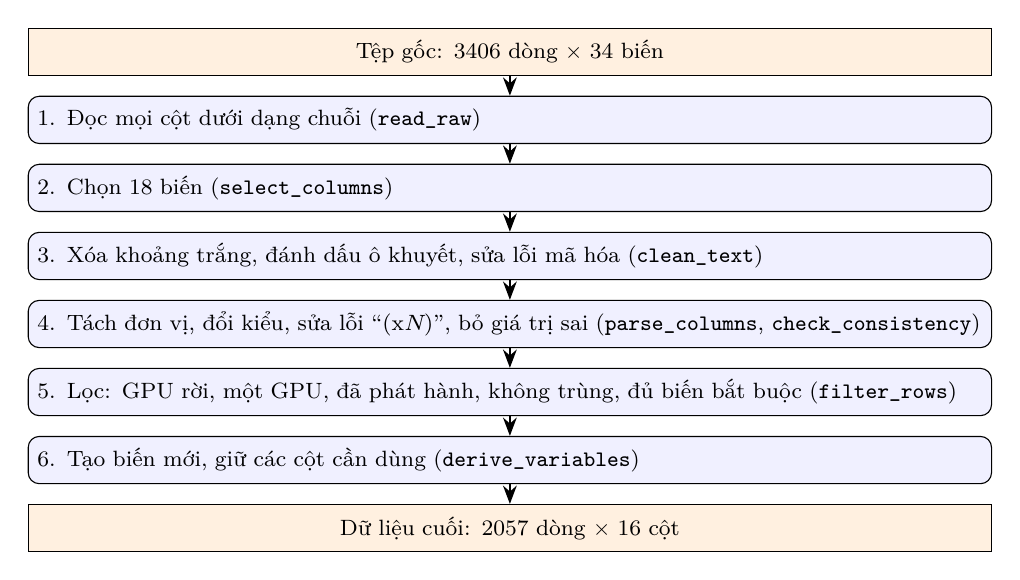
\begin{tikzpicture}[
      node distance=2.5mm,
      box/.style={rectangle, rounded corners, draw, fill=blue!6, text width=12cm,
        align=left, minimum height=6mm, font=\footnotesize},
      io/.style={rectangle, draw, fill=orange!12, text width=12cm, align=center,
        minimum height=6mm, font=\footnotesize},
      arrow/.style={-Stealth, thick}]
    \node[io] (raw) {Tệp gốc: \PreRowsRaw{} dòng $\times$ \PreColsRaw{} biến};
    \node[box, below=of raw] (read) {1. Đọc mọi cột dưới dạng chuỗi
      (\texttt{read\_raw})};
    \node[box, below=of read] (select) {2. Chọn \PreColsSelected{} biến
      (\texttt{select\_columns})};
    \node[box, below=of select] (clean) {3. Xóa khoảng trắng, đánh dấu ô khuyết, sửa
      lỗi mã hóa (\texttt{clean\_text})};
    \node[box, below=of clean] (parse) {4. Tách đơn vị, đổi kiểu, sửa lỗi ``(x$N$)'',
      bỏ giá trị sai (\texttt{parse\_columns}, \texttt{check\_consistency})};
    \node[box, below=of parse] (filter) {5. Lọc: GPU rời, một GPU, đã phát hành, không
      trùng, đủ biến bắt buộc (\texttt{filter\_rows})};
    \node[box, below=of filter] (derive) {6. Tạo biến mới, giữ các cột cần dùng
      (\texttt{derive\_variables})};
    \node[io, below=of derive] (final) {Dữ liệu cuối: \PreRowsFinal{} dòng $\times$
      \PreColsFinal{} cột};
    \foreach \a/\b in {raw/read, read/select, select/clean, clean/parse,
        parse/filter, filter/derive, derive/final}
      \draw[arrow] (\a) -- (\b);
  \end{tikzpicture}
  \caption{Quy trình tiền xử lý (tên hàm Python trong ngoặc)}
  \label{fig:preprocess}
\end{figure}

% ---------------------------------------------------------------------
\subsection{Chọn biến và làm sạch chuỗi (bước 1--3)}

Mọi cột được đọc dưới dạng chuỗi để từng giá trị đều đi qua bước kiểm tra định dạng. Mỗi
dòng được gán mã \texttt{gpu\_id}, là vị trí của dòng trong tệp gốc, để tra ngược khi cần.
Nhóm chọn \PreColsSelected{} biến theo ý nghĩa đối với câu hỏi nghiên cứu, không dựa vào tỉ
lệ khuyết:
{\sloppy
\begin{itemize}
  \item biến mục tiêu \texttt{Max\_Power}; biến giải thích \texttt{TMUs} (số đơn vị xử lý
    texture, đại diện cho quy mô chip), \texttt{Memory}, \texttt{Memory\_Bandwidth},
    \texttt{Process};
  \item biến phụ \texttt{Core\_Speed} (xung nhịp), không bắt buộc phải có
    (mục~\ref{sec:missing});
  \item biến phân nhóm và định danh: \texttt{Name}, \texttt{Manufacturer},
    \texttt{Notebook\_GPU}, \texttt{Memory\_Type}, \texttt{Release\_Date},
    \texttt{Architecture};
  \item biến chỉ dùng khi xử lý: \texttt{Dedicated} (lọc GPU rời), \texttt{ROPs},
    \texttt{Texture\_Rate}, \texttt{Boost\_Clock}, \texttt{Memory\_Bus},
    \texttt{Memory\_Speed} (sửa và kiểm tra lỗi).
\end{itemize}
\par}
{\sloppy Các biến về cổng xuất hình, DirectX, giá bán\ldots{} không liên quan nên bị bỏ.
\texttt{PSU} và \texttt{Power\_Connector} có liên quan nhưng cũng bị bỏ, vì nhà sản xuất chọn
bộ nguồn và đầu cắm \emph{sau khi} đã biết công suất; đưa chúng vào mô hình sẽ làm mô hình dự
đoán tốt một cách giả tạo. \texttt{Pixel\_Rate} mang cùng thông tin về quy mô chip như
\texttt{TMUs}, còn \texttt{Shader} chỉ là phiên bản shader chứ không phải số nhân xử lý.\par}

{\sloppy Trong tệp gốc, ô khuyết không để trống mà ghi chuỗi như \verb|"\n- "| hay
\verb|"\nUnknown Release Date "|. Nếu đọc theo mặc định, \texttt{pandas} đếm được 0 ô khuyết
ở \texttt{Max\_Power}. Bước 3 xóa khoảng trắng ở hai đầu mỗi giá trị, đổi chuỗi rỗng,
\verb|"-"| và \verb|"Unknown Release Date"| thành \texttt{NA} (\PreCellsMarkedMissing{} ô), và
sửa \PreEncodingFixed{} tên card bị lỗi mã hóa (\verb|"²"| thành \verb|"²"|). Bước lọc ở bước 5
vì thế phải đặt sau bước làm sạch.\par}

\begin{lstlisting}[language=Python, caption={Đánh dấu ô khuyết (rút gọn từ hàm \texttt{clean\_text})}]
gpu = gpu.apply(lambda col: col.str.strip())   # "\n01-Mar-2009 " -> "01-Mar-2009"
gpu = gpu.replace(["", "-", "Unknown Release Date"], pd.NA)   # 0 -> 6474 NA cells
\end{lstlisting}

% ---------------------------------------------------------------------
\subsection{Chuyển định dạng và sửa lỗi (bước 4)}

{\sloppy Các biến số được ghi kèm đơn vị, như \verb|"141 Watts"| hay \verb|"64GB/sec"|. Mỗi biến
có một mẫu định dạng riêng để tách phần số. Giá trị không khớp mẫu làm chương trình dừng, nên
không giá trị nào bị đổi sai mà không ai biết. Nếu chỉ xóa mọi ký tự không phải chữ số thì
\verb|"800MB/sec"| sẽ thành 800~GB/s thay vì 0,8~GB/s (\PreBandwidthInMb{} dòng ghi theo
MB/sec). \texttt{Release\_Date} được rút gọn thành năm (\texttt{release\_year}),
\texttt{Dedicated} và \texttt{Notebook\_GPU} thành đúng/sai, \texttt{Manufacturer} và
\texttt{Memory\_Type} thành biến phân loại. Với lỗi dữ liệu, nhóm theo nguyên tắc: giá trị
không thể đúng thì không giữ; sửa nếu tìm được giá trị đúng, nếu không thì bỏ
\cite{vandenbroeck2005}.\par}

{\sloppy\textbf{Lỗi ``(x$N$)'' (sửa).} \PreRopsMultiplier{} dòng ghi \texttt{ROPs} dạng
``$a$ (x$N$)'', nghĩa là $a \times N$; ở đúng các dòng này \texttt{TMUs} và
\texttt{Memory\_Bus} bị ghi chia cho $N$. Ví dụ, GTX~1080~Ti Zotac ghi \verb|"22 (x4)"| ROPs
và 56 TMUs, còn bản tham chiếu ghi 88 ROPs và 224 TMUs $= 56 \times 4$. Hai đẳng thức
kiểm chứng điều này (\texttt{check\_consistency}, cho lệch tối đa 10\%). Thứ nhất, tốc độ texture
$=$ TMUs $\times$ xung nhịp sai ở \PreTextureMismatchBefore{} trong \PreRopsMultiplier{}
dòng trước khi nhân lại (\PreTextureUntestable{} dòng không có xung nhịp để kiểm tra) và
\PreTextureMismatchAfter{} dòng sau đó. Thứ hai, băng thông $=$ độ rộng bus $\times$ tốc độ
bộ nhớ $\times$ hệ số theo loại bộ nhớ sai ở cả \PreRopsMultiplier{} dòng trước khi sửa; sau
khi sửa, cả tệp chỉ còn \PreBandwidthMismatchAfter{} dòng sai, đều là cấu hình SLI bị loại ở
bước 5. Nhóm nhân lại hai cột với $N$; dữ liệu cuối còn \PreRepairedInFinal{} dòng đã sửa
(năm \PreRepairedYears).
\texttt{Max\_Power} không bị ảnh hưởng: ở hai chip có cả dòng lỗi lẫn dòng không lỗi
(GP102 và Baffin PRO), công suất trung vị của hai loại dòng bằng nhau (220~W và 75~W).\par}

\begin{lstlisting}[language=Python, caption={Sửa lỗi ``(x$N$)'' (rút gọn từ hàm \texttt{parse\_columns})}]
# "22 (x4)" -> N = 4;  "88" -> N = 1
n = gpu["ROPs"].str.extract(r"\(x(\d+)\)")[0].astype(float).fillna(1)
gpu["tmus"] = pd.to_numeric(gpu["TMUs"]) * n
bus = gpu["Memory_Bus"].str.removesuffix(" Bit")      # "256 Bit" -> "256"
gpu["memory_bus_bit"] = pd.to_numeric(bus) * n
\end{lstlisting}

\textbf{Công suất 1~W (bỏ).} Radeon HD~6850 Club-3D OC Edition ghi \verb|"1 Watts"|,
trong khi \PreInvalidPowerSiblings{} card khác cùng chip Barts Pro đều ghi
\PreInvalidPowerSiblingWatts~W và tệp gốc ghi cho nó cùng bộ nguồn 500~W như bản tham
chiếu. Giá trị đúng không suy ra được từ chính dòng này, nên ô được đổi thành \texttt{NA}
chứ không điền \PreInvalidPowerSiblingWatts~W. Nhóm không dùng ngưỡng chung kiểu ``dưới
10~W là lỗi'', vì \PreLowPowerLaptopCards{} card laptop ghi dưới 10~W và không có căn cứ để
coi chúng là lỗi. \PrePowerFarFromChipMedian{} card lệch hơn hai lần so với trung vị cùng chip
được giữ nguyên (có thể là thiết kế riêng của hãng gia công) và cần xem lại khi kiểm tra
ngoại lai.

% ---------------------------------------------------------------------
\subsection{Lọc quan sát (bước 5)}

Đề tài nghiên cứu \emph{các card rời dùng một GPU, đã bán ra thị trường}, nên các dòng sau
lần lượt bị loại (Bảng~\ref{tab:rows}):
\begin{itemize}
  \item GPU tích hợp, vì công suất không so sánh được với card rời, và \PreUnknownDedicated{}
    dòng không rõ loại;
  \item cấu hình nhiều GPU, vì công suất ghi là của cả hệ. Nhóm nhận diện chúng qua tên có
    ``SLI'', ``CrossFire'', ``X2''/``GX2'' sau số hiệu, dạng ``A + B'', hoặc thuộc danh sách
    đã biết; mọi trường hợp đã được rà tay để không loại nhầm tên tản nhiệt như ``IceQ X2'';
  \item card chưa phát hành và dòng trùng hoàn toàn;
  \item dòng thiếu biến bắt buộc, tức thiếu bất kỳ cột nào của dữ liệu cuối trừ xung nhịp.
\end{itemize}

\begin{table}[htbp]
  \centering
  \caption{Số dòng còn lại sau từng điều kiện lọc}
  \label{tab:rows}
  \small
  \begin{tabular}{l r r}
    \toprule
    \textbf{Điều kiện lọc} & \textbf{Số dòng} & \textbf{Bị loại} \\
    \midrule
    Dữ liệu gốc & \PreRowsRaw & \\
    Chỉ giữ GPU rời & \PreRowsDedicated
      & \the\numexpr\PreIntegrated+\PreUnknownDedicated\relax \\
    Loại cấu hình nhiều GPU & \PreRowsSingleGpu & \PreMultiGpuRemoved \\
    Loại card chưa phát hành & \PreRowsReleased & \PreUnreleasedRemoved \\
    Loại dòng trùng hoàn toàn & \PreRowsScoped & 0 \\
    Loại dòng thiếu biến bắt buộc & \PreRowsFinal & \PreIncompleteRemoved \\
    \bottomrule
  \end{tabular}
\end{table}

Dữ liệu cuối gồm \PreRowsFinal{} card (\PreDesktop{} desktop, \PreLaptop{} laptop), phát
hành từ \PreReleaseYearMin{} đến \PreReleaseYearMax, chỉ còn Nvidia, AMD và ATI. Mỗi quan
sát là một sản phẩm card. Nhiều hãng gia công bán card dùng chung một chip và thường ghi cùng
công suất, nên các quan sát không hoàn toàn độc lập; các mục sau cần lưu ý điều này khi diễn
giải kiểm định.

% ---------------------------------------------------------------------
\subsection{Tạo biến mới và bộ dữ liệu cuối (bước 6)}

Bước này tạo các biến mà nhiều phân tích cần dùng với cùng một định nghĩa:
\begin{itemize}
  \item \texttt{segment}: Desktop hoặc Laptop;
  \item \texttt{needs\_aux\_power}: công suất trên 75~W, mức tối đa một khe PCIe cấp được;
    biến này chỉ có ý nghĩa với card desktop;
  \item \texttt{memory\_type\_group}: các loại bộ nhớ có dưới 30 card được gộp thành
    ``Other'', còn \PreMemoryTypeGroups{} nhóm. Nhóm ``Other'' chỉ có
    \PreMemoryTypeOtherSize{} card thuộc các công nghệ rất khác nhau, nên chỉ dùng để mô tả;
  \item \texttt{texture\_rate\_per\_watt}: hiệu quả năng lượng, bằng tốc độ xử lý texture
    chia cho công suất.
\end{itemize}
Dữ liệu được lưu dưới dạng \texttt{pandas.DataFrame}, mỗi dòng một card;
Bảng~\ref{tab:columns} liệt kê các cột.

\begin{table}[htbp]
  \centering
  \caption{Các cột của bộ dữ liệu cuối và tỉ lệ khuyết trước khi loại dòng khuyết}
  \label{tab:columns}
  \small
  \begin{tabular}{l >{\ttfamily}l l r}
    \toprule
    \textbf{Vai trò} & \normalfont\textbf{Cột} & \textbf{Kiểu} & \textbf{Khuyết (\%)}$^{*}$ \\
    \midrule
    Định danh & gpu\_id, name & số nguyên, chuỗi & \PreMissingPctName \\
    Biến mục tiêu & max\_power\_w & số thực & \PreMissingPctMaxPowerW \\
    Tạo từ mục tiêu & needs\_aux\_power & đúng/sai & \PreMissingPctNeedsAuxPower \\
                    & texture\_rate\_per\_watt & số thực & \PreMissingPctTextureRatePerWatt \\
    Biến giải thích & tmus & số đếm & \PreMissingPctTmus \\
                    & memory\_bandwidth\_gb\_s & số thực & \PreMissingPctMemoryBandwidthGbS \\
                    & memory\_mb & số thực & \PreMissingPctMemoryMb \\
                    & process\_nm & số thực & \PreMissingPctProcessNm \\
    Biến phụ (được khuyết) & core\_speed\_mhz & số thực & \PreMissingPctCoreSpeedMhz \\
    Biến phân nhóm & manufacturer & phân loại & \PreMissingPctManufacturer \\
                   & segment & phân loại & \PreMissingPctSegment \\
                   & memory\_type(\_group) & phân loại & \PreMissingPctMemoryType \\
    Thời gian, chip & release\_year & số nguyên & \PreMissingPctReleaseYear \\
                    & architecture & chuỗi & \PreMissingPctArchitecture \\
    \bottomrule
  \end{tabular}

  \smallskip
  {\footnotesize $^{*}$ Trên \PreRowsScoped{} dòng thuộc phạm vi đề tài. Sau khi loại,
    chỉ \texttt{core\_speed\_mhz} còn khuyết (\PreCoreMissingInFinal{} dòng,
    \PreCoreMissingInFinalPct\%).\par}
\end{table}

% ---------------------------------------------------------------------
\subsection{Xử lý dữ liệu khuyết}
\label{sec:missing}

Nhóm không điền giá trị nào: dòng thiếu một biến bắt buộc bị loại, riêng xung nhịp được
phép khuyết. Có \PreRowsIncomplete{} dòng (\PreRowsIncompletePct\%) bị loại, trong đó
\PrePowerMissing{} dòng thiếu chính công suất, tức biến mục tiêu. Chỉ
\PrePowerRowsLostByDropAll{} dòng có công suất mà bị loại vì thiếu biến khác.

Điền trung bình hay trung vị là tự tạo số liệu, và làm kết quả trông chắc chắn hơn thực tế.
Nếu điền trung vị cho công suất, \PrePowerAtMedianImputed\% số card sẽ có cùng một giá trị và
độ lệch chuẩn giảm từ \PrePowerSdDropped{} xuống \PrePowerSdImputed~W. Điền cho biến giải thích
cũng làm sai lệch mối liên hệ với công suất \cite{donders2006}. Tài liệu này cũng lưu ý rằng
loại dòng có thể gây lệch khi ô khuyết không ngẫu nhiên, và khuyến nghị điền nhiều lần
(multiple imputation). Phương pháp đó vượt ngoài chương trình môn học, nên nhóm kiểm tra trực
tiếp mức lệch do loại dòng ở phần dưới.

Xung nhịp không bắt buộc vì nếu bắt buộc, dữ liệu chỉ còn \PreRowsIfCoreRequired{} dòng,
mất thêm \PreCoreMissingInFinal{} card đủ mọi thông số khác. Các card này có công suất thấp hơn
(\PreCoreMissingPowerMean~W so với \PreCoreKnownPowerMean~W), nên bỏ chúng sẽ làm dữ liệu lệch
thêm về card công suất lớn. Xung nhịp có liên hệ với công suất: trong cùng một chip, xung nhịp
cao hơn 1\% đi kèm công suất cao hơn khoảng \PreCoreWithinChipElasticity\% (ước lượng mô tả).
Giữa các chip, xung nhịp lại đi cùng tiến trình ($r = \PreCoreProcessCorr$) và năm phát hành
($r = \PreCoreYearCorr$); hai biến này giải thích khoảng \PreCoreExplainedPct\% sự khác nhau về
xung nhịp, nên khó tách riêng ảnh hưởng của nó. Vì vậy xung nhịp không nằm trong mô hình chính.
Hệ số của tiến trình khi đó cần được hiểu là đã bao gồm phần đi kèm với xung nhịp. Đây là lựa
chọn đưa ra sau khi đã xem dữ liệu.

Ô khuyết không xảy ra ngẫu nhiên. Card càng cũ càng hay thiếu công suất
(Bảng~\ref{tab:missing-period}): năm phát hành trung bình của card khuyết là
\PreMissingMeanYear{} so với \PreObservedMeanYear{} ($z = \PreMissingYearZ$,
$p$ \PreMissingYearP), và tỉ lệ AMD cao hơn (\PreMissingAmdPct\% so với
\PreObservedAmdPct\%, trong số card Nvidia và AMD). Các kiểm định $z$ này coi mỗi card là
độc lập nên chỉ dùng để mô tả. Dữ liệu cuối vì thế nghiêng về card đời mới: chỉ có
\PreRowsBeforeTwoThousandSix{} card trước năm 2006, và các dòng có công suất nhưng bị loại có
công suất trung bình \PreLostPowerMean~W, thấp hơn \PreFinalPowerMean~W của các dòng được giữ.

\begin{table}[htbp]
  \centering
  \caption{Tỉ lệ khuyết công suất và tỉ lệ bị loại theo năm phát hành
    (\PreRowsScoped{} dòng trước khi loại dòng khuyết)}
  \label{tab:missing-period}
  \small
  \begin{tabular}{l r r r}
    \toprule
    \textbf{Năm phát hành} & \textbf{Số card} & \textbf{Khuyết công suất (\%)}
      & \textbf{Bị loại (\%)} \\
    \midrule
    \csname @@input\endcsname generated/preprocessing_missing_by_period.tex
    Không rõ năm & \PreUnknownYearRows & \PreUnknownYearPowerMissingPct
      & \PreUnknownYearDroppedPct \\
    \bottomrule
  \end{tabular}
\end{table}


Bộ dữ liệu cuối có công suất trung bình cao hơn một chút so với mọi card có ghi công suất
(\PreFinalPowerMean{} so với \PreAllPowerMean~W, Bảng~\ref{tab:power-groups}). Các kết luận ở
mục sau vì vậy chỉ đại diện cho GPU rời có đủ thông số, chủ yếu phát hành từ 2006 đến
\PreReleaseYearMax. Chênh lệch giữa desktop và laptop ổn định trên cả hai tập (desktop gấp
khoảng ba lần). Chênh lệch Nvidia trừ AMD thì đổi từ $\PreNvidiaMinusAmdFinal$ thành
$\PreNvidiaMinusAmdAll$~W, nên kết luận về hãng cần được kiểm tra trên cả hai tập.

\begin{table}[htbp]
  \centering
  \caption{Công suất (W) trên bộ dữ liệu cuối và trên mọi card có ghi công suất}
  \label{tab:power-groups}
  \small
  \begin{tabular}{l r r r r r r}
    \toprule
    & \multicolumn{3}{c}{\textbf{Bộ dữ liệu cuối}}
      & \multicolumn{3}{c}{\textbf{Mọi card có công suất}} \\
    \cmidrule(lr){2-4} \cmidrule(lr){5-7}
    \textbf{Nhóm} & \textbf{Số card} & \textbf{TB} & \textbf{Trung vị}
      & \textbf{Số card} & \textbf{TB} & \textbf{Trung vị} \\
    \midrule
    Tất cả & \PreRowsFinal & \PreFinalPowerMean & \PreFinalPowerMedian
      & \PreRowsWithPower & \PreAllPowerMean & \PreAllPowerMedian \\
    \midrule
    \csname @@input\endcsname generated/preprocessing_power_by_group.tex
    \bottomrule
  \end{tabular}
\end{table}


% Mục 4: Thống kê mô tả (dữ liệu 2057 dòng)
\clearpage
\section{Thống kê mô tả}

\subsection{Các giá trị đặc trưng mẫu}

Để khảo sát các đặc trưng xu hướng trung tâm và độ phân tán của các thông số kỹ thuật GPU rời (tệp \texttt{gpus\_analysis.parquet} gồm $n = 2057$ quan trắc), nhóm sử dụng các chỉ số thống kê gồm: giá trị nhỏ nhất (\textbf{Min}), giá trị lớn nhất (\textbf{Max}), giá trị trung bình (\textbf{Mean}), độ lệch chuẩn (\textbf{SD}), trung vị (\textbf{Median}), tứ phân vị thứ nhất (\textbf{Q1}), tứ phân vị thứ ba (\textbf{Q3}) và khoảng tứ phân vị (\textbf{IQR}). Biến \texttt{core\_speed\_mhz} được loại khỏi tập phân tích chính do tỷ lệ khuyết dữ liệu cao và không giữ vai trò quyết định độc lập trong mô hình công suất.

Trong Python, các đại lượng này được tính toán thông qua thư viện \texttt{pandas} và \texttt{numpy}:

\begin{lstlisting}[language=Python]
import pandas as pd
import numpy as np

# Doc du lieu GPU da duoc lam sach va an danh muc hang khong co du lieu
df = pd.read_parquet("data/processed/gpus_analysis.parquet")
df['manufacturer'] = df['manufacturer'].cat.remove_unused_categories()

# Danh sach 6 bien dinh luong chinh
num_cols = [
    'max_power_w', 'process_nm', 'memory_bandwidth_gb_s',
    'memory_mb', 'tmus', 'texture_rate_per_watt'
]

# Tinh toan cac gia tri dac trung mau
stats_df = pd.DataFrame({
    'Min': df[num_cols].min(),
    'Max': df[num_cols].max(),
    'Mean': df[num_cols].mean(),
    'SD': df[num_cols].std(),
    'Median': df[num_cols].median(),
    'Q1': df[num_cols].quantile(0.25),
    'Q3': df[num_cols].quantile(0.75),
    'IQR': df[num_cols].quantile(0.75) - df[num_cols].quantile(0.25)
}).round(2)

print(stats_df)
\end{lstlisting}

Ý nghĩa chi tiết của 6 biến kỹ thuật định lượng đại diện cho GPU trong bài phân tích bao gồm:
\begin{itemize}\tightlist
    \item \texttt{max\_power\_w} \textbf{(Max Power -- Watt):} Công suất tiêu thụ điện năng tối đa của card đồ họa khi hoạt động ở mức tải cao nhất.
    \item \texttt{process\_nm} \textbf{(Process Size -- nm):} Kích thước tiến trình sản xuất bán dẫn của chip GPU (đơn vị nanomet). Tiến trình càng nhỏ thể hiện công nghệ sản xuất càng tiên tiến và tiết kiệm điện.
    \item \texttt{memory\_bandwidth\_gb\_s} \textbf{(Memory Bandwidth -- GB/s):} Băng thông bộ nhớ VRAM, phản ánh tốc độ truyền dữ liệu giữa bộ nhớ đồ họa và nhân GPU trong một giây.
    \item \texttt{memory\_mb} \textbf{(Memory Size -- MB):} Dung lượng bộ nhớ đồ họa VRAM (đơn vị Megabyte), cho biết khả năng lưu trữ dữ liệu hình ảnh, kết cấu (texture) của card.
    \item \texttt{tmus} \textbf{(Texture Mapping Units):} Số lượng đơn vị xử lý phủ vân bề mặt hình ảnh 3D trong cấu trúc phần cứng của GPU.
    \item \texttt{texture\_rate\_per\_watt} \textbf{(Texture Rate per Watt):} Tỷ lệ hiệu suất xử lý phủ vân bề mặt trên mỗi Watt công suất tiêu thụ, phản ánh hiệu suất năng lượng của GPU.
\end{itemize}

Bảng~\ref{tab:gpu_descriptive_stats} tổng hợp các giá trị đặc trưng thu được từ tập dữ liệu GPU sau tiền xử lý.

\begin{table}[H]
    \centering
    \footnotesize
    \setlength{\tabcolsep}{4.5pt}
    \caption{Các giá trị đặc trưng mẫu của các biến định lượng kỹ thuật GPU}
    \label{tab:gpu_descriptive_stats}
    \renewcommand{\arraystretch}{1.3}
    \resizebox{\linewidth}{!}{%
    \begin{tabular}{|l|c|c|c|c|c|c|c|c|}
        \hline
        \rowcolor{TableHead}
        \textbf{Tên biến} & \textbf{Min} & \textbf{Max} & \textbf{Mean} & \textbf{SD} & \textbf{Median} & \textbf{Q1} & \textbf{Q3} & \textbf{IQR} \\ \hline
        \texttt{max\_power\_w} (Watts) & 5.00 & 375.00 & 124.93 & 76.94 & 120.00 & 64.00 & 171.00 & 107.00 \\ \hline
        \texttt{process\_nm} (nm) & 14.00 & 150.00 & 30.93 & 13.63 & 28.00 & 28.00 & 40.00 & 12.00 \\ \hline
        \texttt{memory\_bandwidth\_gb\_s} (GB/s) & 4.00 & 547.20 & 144.86 & 110.73 & 112.20 & 57.70 & 224.00 & 166.30 \\ \hline
        \texttt{memory\_mb} (MB) & 128.00 & 16384.00 & 3063.13 & 2531.27 & 2048.00 & 1024.00 & 4096.00 & 3072.00 \\ \hline
        \texttt{tmus} & 4.00 & 256.00 & 76.58 & 57.33 & 64.00 & 32.00 & 120.00 & 88.00 \\ \hline
        \texttt{texture\_rate\_per\_watt} & 0.03 & 1.92 & 0.66 & 0.37 & 0.59 & 0.37 & 0.84 & 0.47 \\ \hline
    \end{tabular}%
    }
\end{table}

Bên cạnh đó, đối với biến phân loại định tính Hãng sản xuất (\texttt{manufacturer}) sau khi loại bỏ các hãng không có dữ liệu GPU rời trong mẫu (như Intel), bảng tần số và tần suất được tổng hợp ở Bảng~\ref{tab:freq_manufacturer}.

\begin{table}[H]
    \centering
    \small
    \caption{Bảng tần số và tần suất của biến Hãng sản xuất}
    \label{tab:freq_manufacturer}
    \renewcommand{\arraystretch}{1.25}
    \begin{tabular}{|l|c|c|c|}
        \hline
        \rowcolor{TableHead}
        \textbf{Hãng sản xuất} & \textbf{Số lượng mẫu (Tần số)} & \textbf{Tỷ lệ (\%)} & \textbf{Tỷ lệ tích lũy (\%)} \\ \hline
        Nvidia & 1186 & 57.66\% & 57.66\% \\ \hline
        AMD & 794 & 38.60\% & 96.26\% \\ \hline
        ATI & 77 & 3.74\% & 100.00\% \\ \hline
        \textbf{Tổng cộng} & \textbf{2057} & \textbf{100.00\%} & -- \\ \hline
    \end{tabular}
\end{table}

\subsection{Đồ thị mô tả dữ liệu}

Nhằm quan sát trực quan dạng phân phối của biến mục tiêu \texttt{max\_power\_w}, so sánh sự khác biệt công suất giữa các phân khúc thiết bị (\texttt{segment}) và đánh giá mối tương quan giữa các thông số phần cứng, nhóm trực quan hóa dữ liệu bằng ba đồ thị dưới đây.

\subsubsection{Biểu đồ tần suất công suất tiêu thụ tối đa (Histogram)}

Mã nguồn Python vẽ biểu đồ tần suất Histogram cho biến \texttt{max\_power\_w} trên thang đo gốc (Watts) và thang đo Logarithm tự nhiên ($\ln$):

\begin{lstlisting}[language=Python]
# Graph 1: Histogram Max_Power (Goc vs Log)
fig, axes = plt.subplots(1, 2, figsize=(11, 4.5))
sns.histplot(df['max_power_w'], kde=True, ax=axes[0], color='skyblue')
axes[0].set_title('Phan bo Max_Power (Watts)')

sns.histplot(np.log(df['max_power_w']), kde=True, ax=axes[1], color='salmon')
axes[1].set_title('Phan bo ln(Max_Power)')
plt.tight_layout()
plt.savefig(CURRENT_DIR / "histogram_max_power.png", dpi=300)
plt.close()
\end{lstlisting}

\begin{figure}[H]
    \centering
    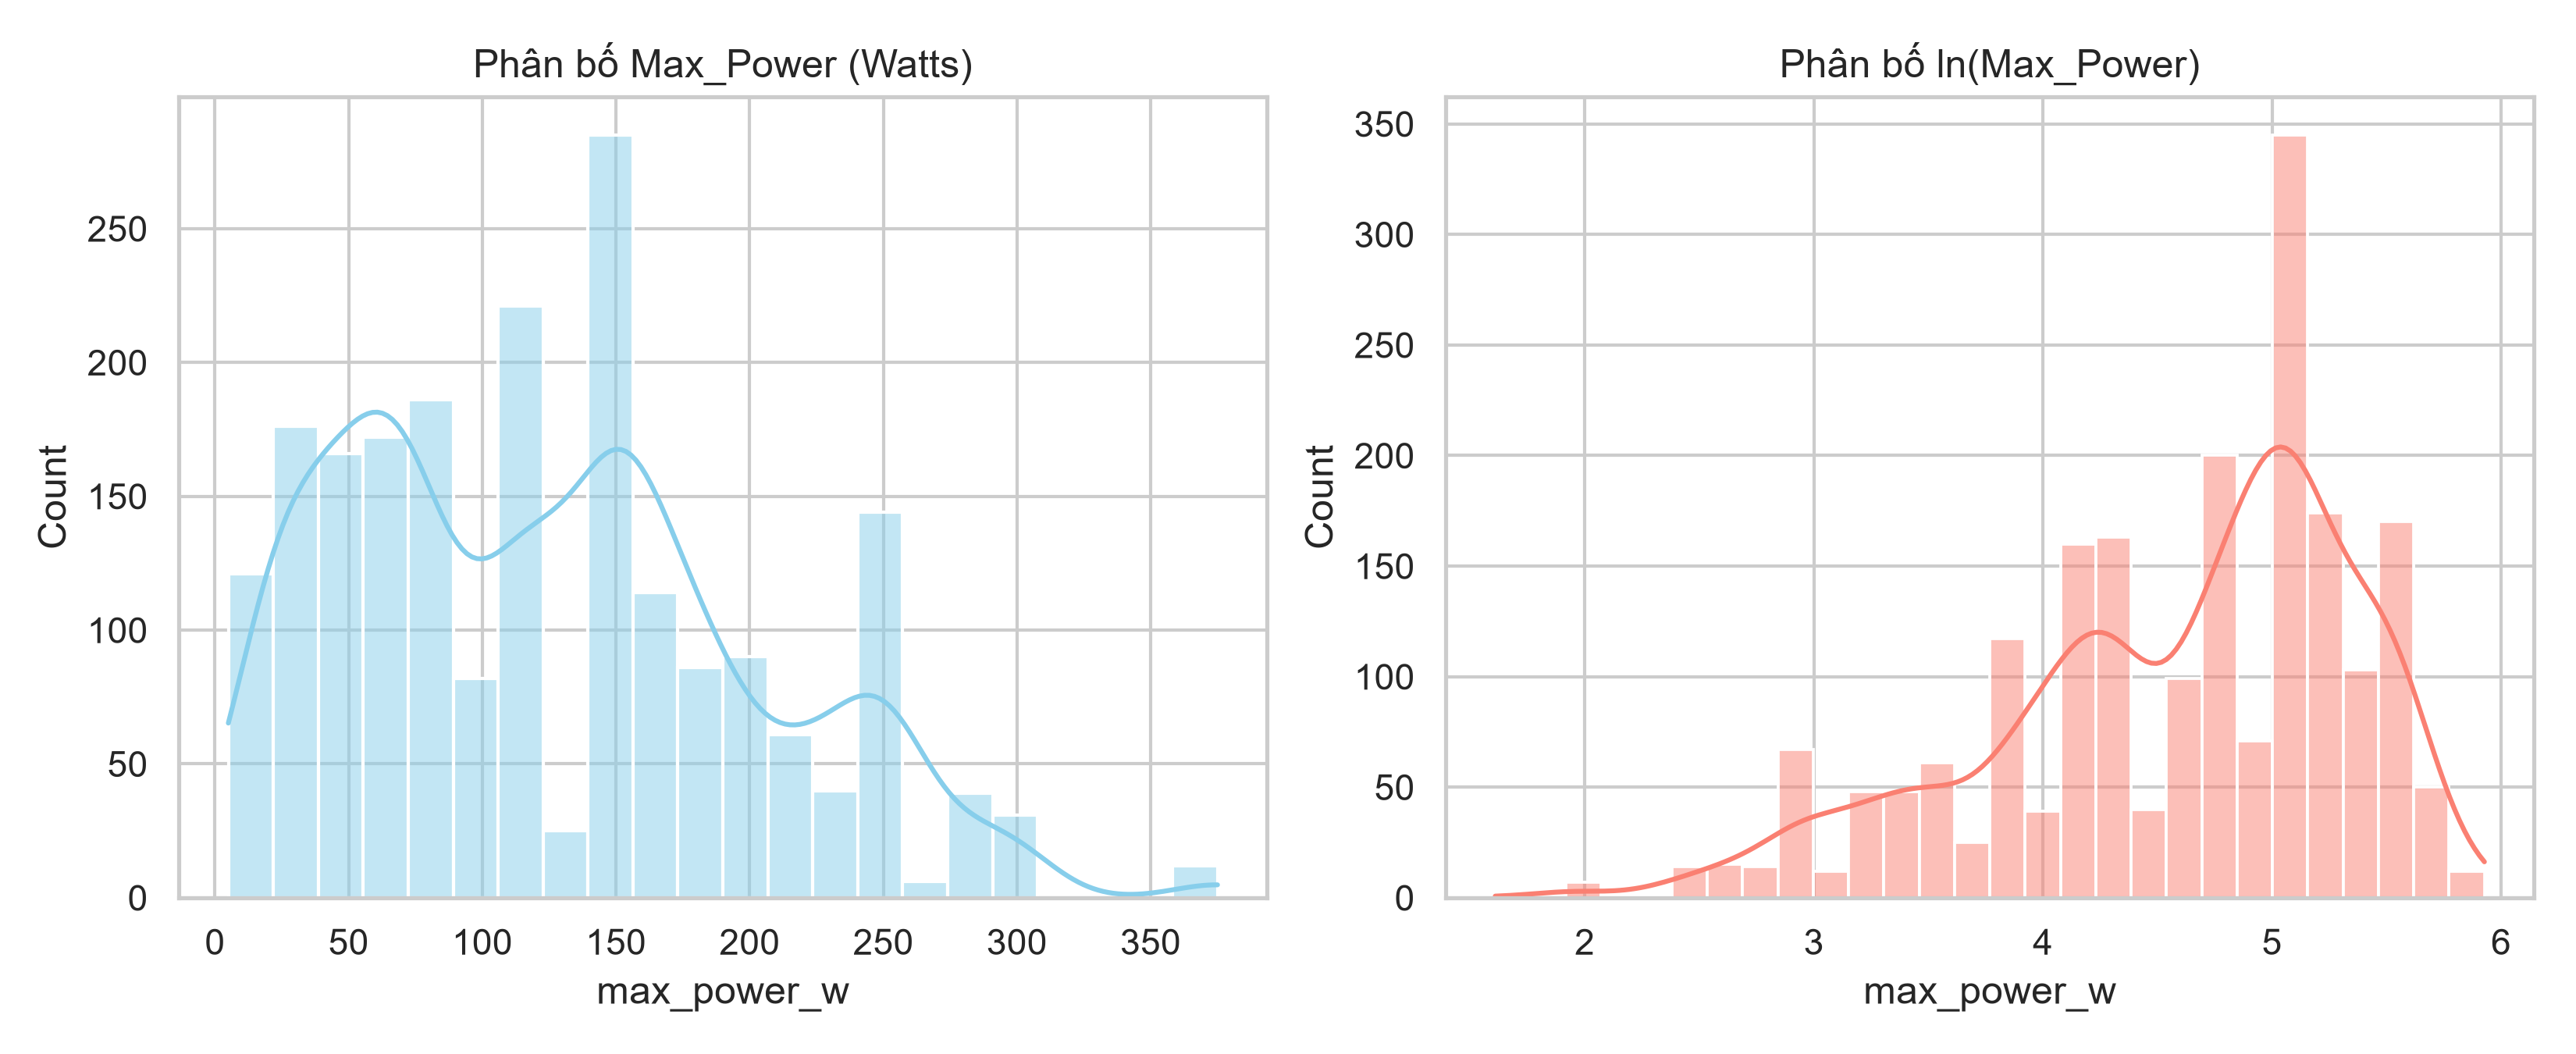
\includegraphics[width=0.88\textwidth]{figures/histogram_max_power.png}
    \caption{Biểu đồ phân bố công suất tiêu thụ tối đa \texttt{max\_power\_w} (Thang đo gốc Watts và thang đo Logarithm)}
    \label{fig:hist_max_power}
\end{figure}

\textbf{Nhận xét biểu đồ Histogram:}
\begin{itemize}\tightlist
    \item \textbf{Trên thang đo gốc (Watts):} Phân bố của \texttt{max\_power\_w} lệch phải rõ rệt (đỉnh tập trung về phía bên trái), cho thấy phần lớn các mẫu GPU nằm ở phân khúc công suất thấp và phổ thông (trung vị đạt $120.00\text{ W}$ và $75\%$ số mẫu có công suất từ $171.00\text{ W}$ trở xuống, khoảng tứ phân vị $\text{IQR} = 107.00\text{ W}$). Phần đuôi kéo dài sang bên phải đại diện cho nhóm card đồ họa cao cấp có mức tiêu thụ điện năng lớn từ $250\text{ W}$ đến $375\text{ W}$.
    \item \textbf{Sau khi biến đổi Logarithm ($\ln$):} Dữ liệu được dàn trải đều hơn, giảm thiểu độ lệch phải và co cụm lại quanh vùng trung tâm từ $4.0$ đến $5.5$, giúp phân bố tiệm cận dạng cân đối hơn để phục vụ các bước kiểm định và hồi quy tuyến tính.
\end{itemize}

\subsubsection{Biểu đồ hộp so sánh công suất tiêu thụ (Boxplot)}

Mã nguồn Python vẽ biểu đồ hộp Boxplot so sánh phân bố công suất \texttt{max\_power\_w} giữa hai phân khúc thiết bị Desktop và Laptop (\texttt{segment}) theo từng Hãng sản xuất (\texttt{manufacturer}):

\begin{lstlisting}[language=Python]
# Graph 2: Boxplot Desktop vs Laptop
plt.figure(figsize=(8, 4.5))
sns.boxplot(x='manufacturer', y='max_power_w', hue='segment', data=df, palette='Set2')
plt.title('So sanh Max_Power giua Desktop va Laptop')
plt.tight_layout()
plt.savefig(CURRENT_DIR / "boxplot_max_power.png", dpi=300)
plt.close()
\end{lstlisting}

\begin{figure}[H]
    \centering
    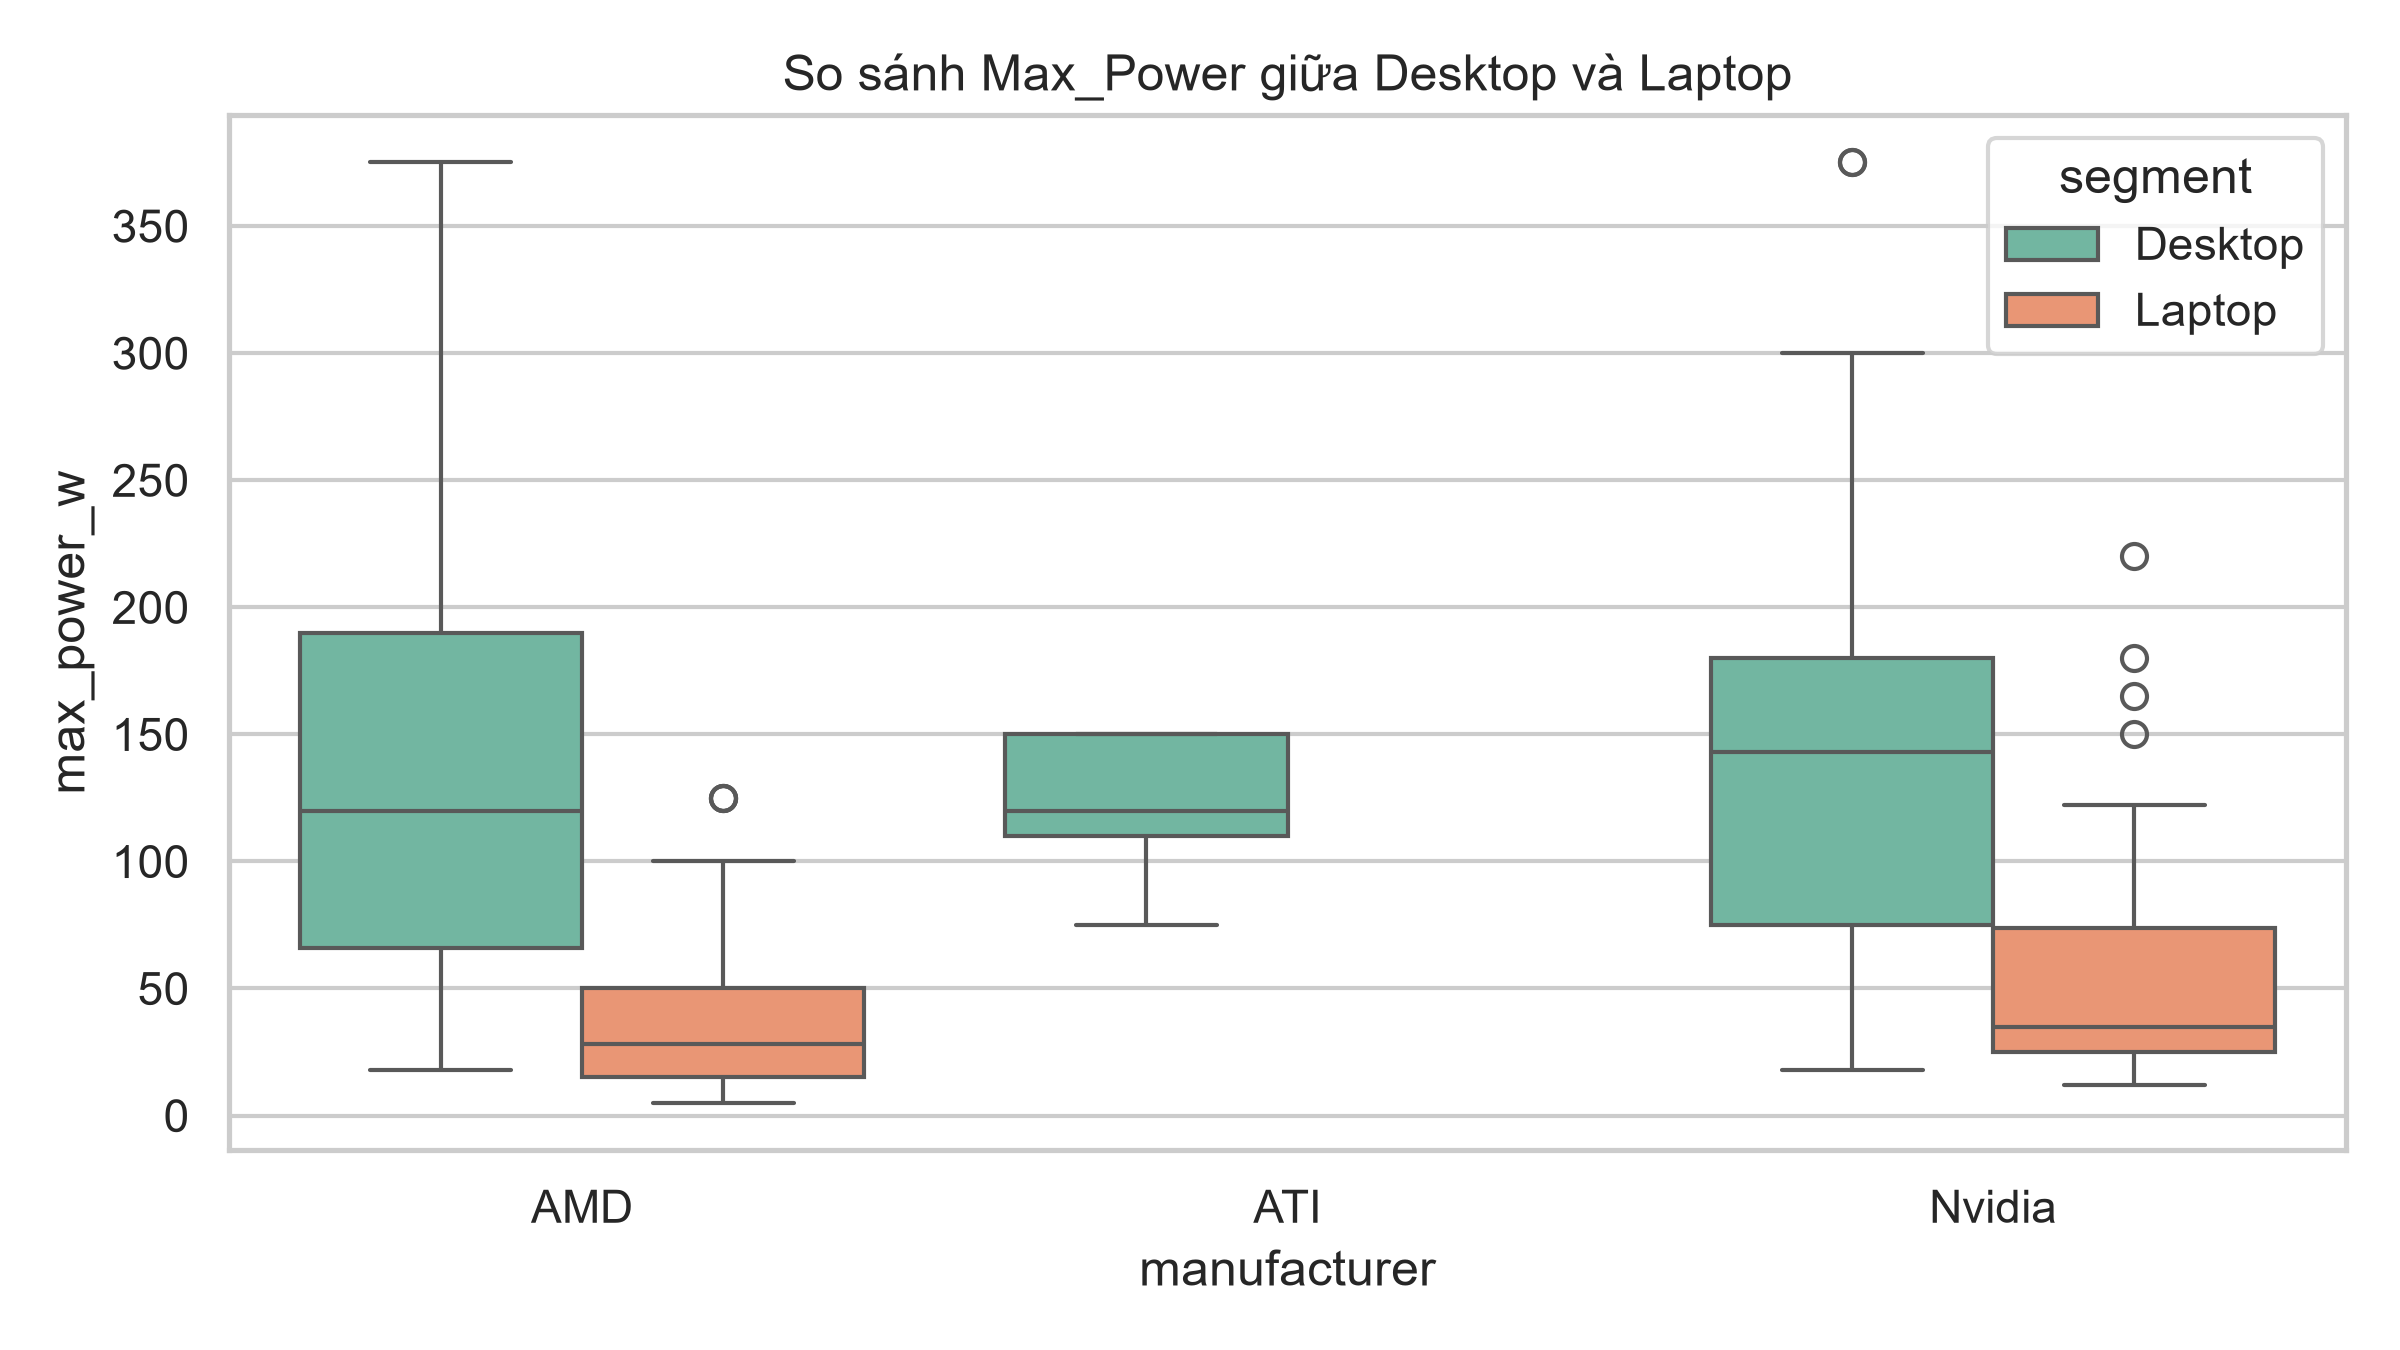
\includegraphics[width=0.82\textwidth]{figures/boxplot_max_power.png}
    \caption{Biểu đồ hộp so sánh công suất \texttt{max\_power\_w} theo Hãng sản xuất và Phân khúc Desktop/Laptop}
    \label{fig:boxplot_max_power}
\end{figure}

\textbf{Nhận xét biểu đồ Boxplot:}
\begin{itemize}\tightlist
    \item \textbf{Theo phân khúc thiết bị:} Ở cả AMD và Nvidia, phân khúc Laptop có mức trung vị (khoảng $28\text{--}35\text{ W}$) và khoảng tứ phân vị $\text{IQR}$ nhỏ hơn đáng kể so với phân khúc Desktop (trung vị khoảng $120\text{--}143\text{ W}$), phản ánh giới hạn nghiêm ngặt về nguồn cấp và tản nhiệt trên thiết bị di động. Riêng hãng ATI chỉ ghi nhận các mẫu thuộc phân khúc Desktop (do thương hiệu này đã được AMD sáp nhập và ngừng phát triển các dòng chip di động thế hệ mới).
    \item \textbf{Theo hãng sản xuất và giá trị ngoại lệ:} AMD và Nvidia có dải công suất trải rộng từ các dòng phổ thông đến cao cấp (lên tới $375\text{ W}$). Xuất hiện một số điểm ngoại lệ phía trên rào chắn $Q_3 + 1.5\text{IQR}$ ở phân khúc Laptop của AMD, Nvidia và phân khúc Desktop của Nvidia, đại diện cho các mẫu GPU hiệu năng cao dành cho máy trạm hoặc laptop chơi game chuyên dụng.
\end{itemize}

\subsubsection{Biểu đồ ma trận hệ số tương quan (Correlation Heatmap)}

Đoạn mã Python tính toán ma trận hệ số tương quan Pearson ($r_{XY}$) giữa 6 biến định lượng và trực quan hóa bằng biểu đồ nhiệt (Heatmap):

\begin{lstlisting}[language=Python]
# Graph 3: Correlation Matrix Heatmap
plt.figure(figsize=(7, 5))
sns.heatmap(df[num_cols].corr(), annot=True, fmt=".2f", cmap='coolwarm', vmin=-1, vmax=1)
plt.title('Ma tran he so tuong quan Pearson')
plt.tight_layout()
plt.savefig(CURRENT_DIR / "correlation_matrix.png", dpi=300)
plt.close()
\end{lstlisting}

\begin{figure}[H]
    \centering
    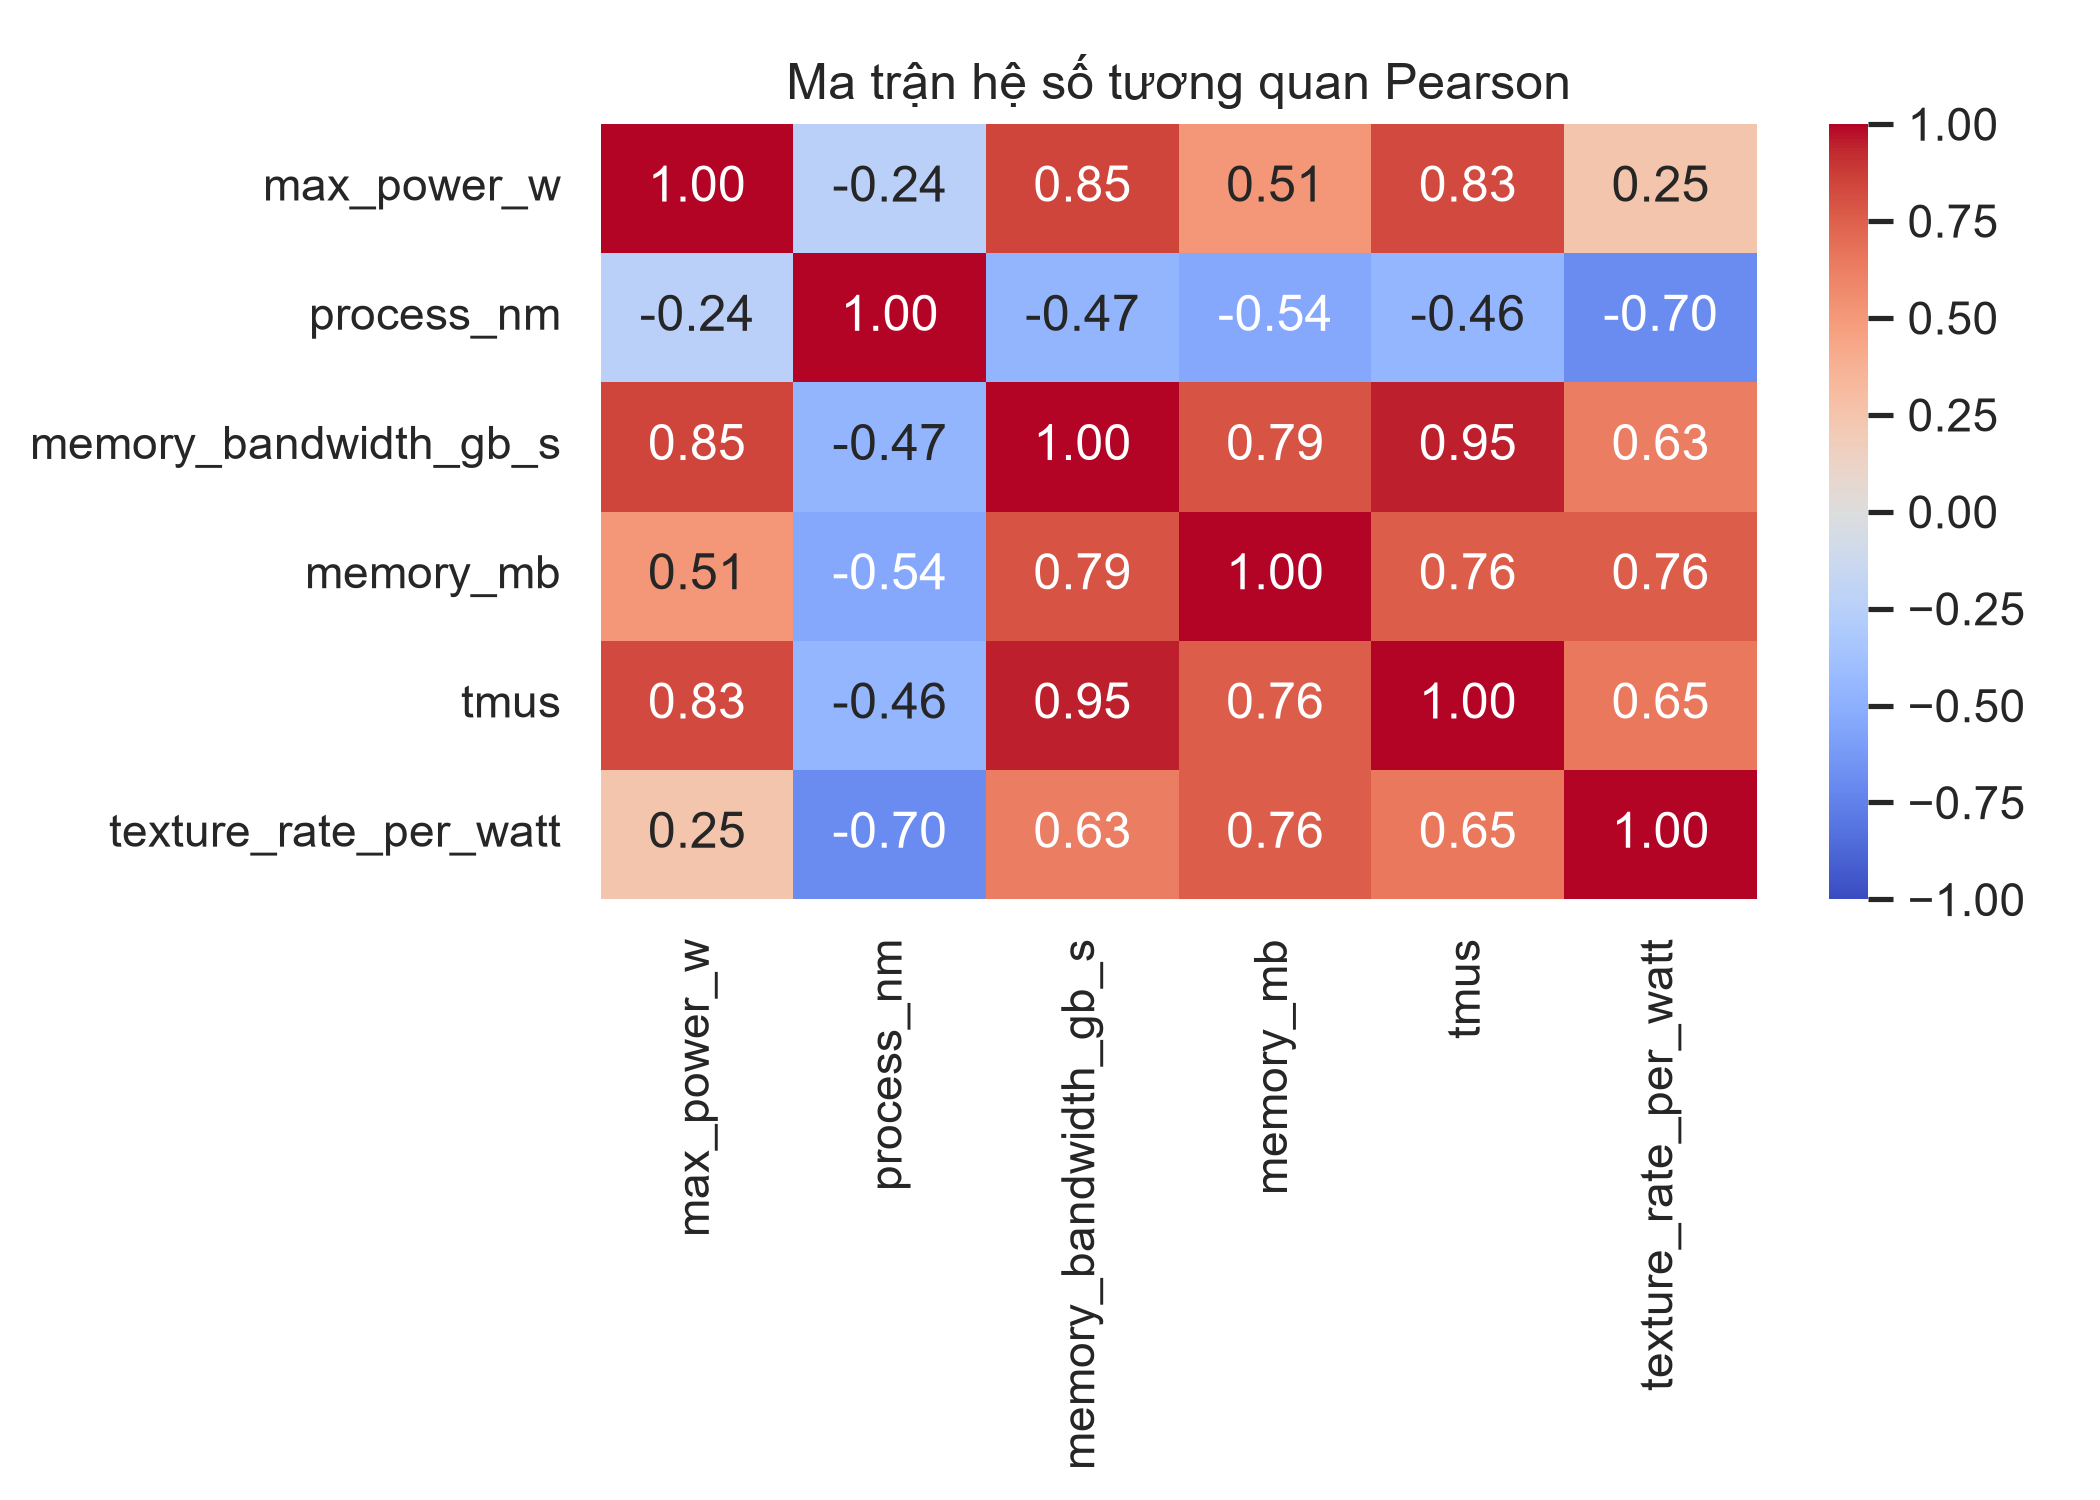
\includegraphics[width=0.76\textwidth]{figures/correlation_matrix.png}
    \caption{Ma trận hệ số tương quan Pearson giữa 6 biến kỹ thuật định lượng}
    \label{fig:corr_matrix}
\end{figure}

\textbf{Nhận xét mối liên hệ tương quan:}
\begin{itemize}\tightlist
    \item \textbf{Tương quan với biến mục tiêu \texttt{max\_power\_w}:} Công suất tiêu thụ tối đa có tương quan thuận rất mạnh với Băng thông bộ nhớ \texttt{memory\_bandwidth\_gb\_s} ($r = 0.85$) và Số đơn vị xử lý phủ vân bề mặt \texttt{tmus} ($r = 0.83$), cùng mức tương quan trung bình với Dung lượng bộ nhớ \texttt{memory\_mb} ($r = 0.51$). Điều này cho thấy các card đồ họa có quy mô nhân xử lý lớn và băng thông bộ nhớ cao đòi hỏi công suất cấp nguồn lớn hơn rõ rệt.
    \item \textbf{Tương quan giữa các biến kỹ thuật và hiệu suất năng lượng:} Kích thước tiến trình bán dẫn \texttt{process\_nm} có tương quan nghịch mạnh với Hiệu suất năng lượng \texttt{texture\_rate\_per\_watt} ($r = -0.70$) và Dung lượng bộ nhớ \texttt{memory\_mb} ($r = -0.54$), chứng minh việc thu nhỏ tiến trình sản xuất giúp nâng cao đáng kể hiệu năng xử lý trên mỗi Watt điện năng tiêu thụ. Bên cạnh đó, \texttt{tmus} và \texttt{memory\_bandwidth\_gb\_s} có tương quan thuận rất chặt chẽ ($r = 0.95$), phản ánh sự cân đối đồng bộ giữa năng lực tính toán của nhân đồ họa và tốc độ truyền tải bộ nhớ.
\end{itemize}

\subsection{Tổng kết đặc điểm dữ liệu}

Từ các kết quả thống kê mô tả và trực quan hóa trên tập dữ liệu $n = 2057$ GPU rời, có thể rút ra những đặc điểm chính sau:
\begin{itemize}\tightlist
    \item \textbf{Quy mô và cơ cấu mẫu:} Dữ liệu tập trung chủ yếu vào hai nhà sản xuất lớn là Nvidia ($57.66\%$) và AMD ($38.60\%$), chiếm hơn $96\%$ tổng số mẫu nghiên cứu; phần còn lại thuộc về ATI ($3.74\%$).
    \item \textbf{Đặc điểm phân phối công suất:} Biến mục tiêu \texttt{max\_power\_w} biến thiên rộng từ $5.00\text{ W}$ đến $375.00\text{ W}$ với phân phối lệch phải ($\text{Mean} = 124.93\text{ W} > \text{Median} = 120.00\text{ W}$, $\text{IQR} = 107.00\text{ W}$). Việc biến đổi sang thang đo $\ln(\texttt{max\_power\_w})$ giúp phân bố dữ liệu cân đối hơn, phù hợp cho các phân tích suy diễn tiếp theo.
    \item \textbf{Sự phân hóa theo phân khúc và thông số phần cứng:} Công suất tiêu thụ có sự phân tầng rõ rệt giữa hai nhóm thiết bị Desktop và Laptop, đồng thời chịu tác động tuyến tính thuận rất mạnh từ băng thông bộ nhớ ($r = 0.85$) và số lượng đơn vị TMUs ($r = 0.83$).
\end{itemize}


% Mục 5: Thống kê suy diễn (gồm đủ 5 phương pháp)
\clearpage
\section{Thống kê suy diễn}
\label{sec:inferential}

% 5.1 Kiểm định 1 mẫu
\subsection{Bài toán kiểm định trung bình một mẫu}

\subsubsection{Đề xuất phương pháp}

Theo chuẩn kỹ thuật phần cứng máy tính, khe cắm mở rộng PCIe~x16 trên bo mạch chủ cung cấp công suất tối đa $75$\,W; các card đồ họa vượt ngưỡng này bắt buộc phải sử dụng thêm đầu cấp nguồn phụ từ bộ nguồn (PSU)[cite: 6]. Do đó, việc kiểm định mức công suất thiết kế trung bình của thị trường GPU rời so với ngưỡng $75$\,W giúp đánh giá xu hướng thiết kế hệ thống cấp điện của phần cứng đồ họa.

\textbf{Bài toán.} Với mức ý nghĩa $\alpha = 0{,}05$ (độ tin cậy $95\%$), công suất thiết kế tối đa trung bình (\texttt{max\_power\_w}) của GPU rời có lớn hơn ngưỡng $75$\,W của khe PCIe hay không?

Bài toán sử dụng toàn bộ $n = 2\,057$ GPU rời trong tập dữ liệu sạch (\texttt{gpus\_\allowbreak{}analysis.parquet})[cite: 6]. Từ các đặc trưng thống kê mẫu, ta có trung bình mẫu $\bar{x} = 124{,}93$\,W, độ lệch chuẩn mẫu $s = 76{,}94$\,W, trung vị $120{,}00$\,W, $\text{IQR} = 107{,}00$\,W và sai số chuẩn của trung bình mẫu là:
\[
  SE = \frac{s}{\sqrt{n}} = \frac{76{,}94}{\sqrt{2\,057}} = 1{,}70\text{\,W}.
\]

Gọi $\mu$ là công suất thiết kế tối đa trung bình tổng thể của GPU rời. Cặp giả thuyết kiểm định một phía bên phải được thiết lập như sau:
\[
  H_0: \mu = 75\text{\,W}, \qquad H_1: \mu > 75\text{\,W}.
\]

\subsubsection{Phân tích kiểm định một mẫu}

\paragraph{Kiểm tra điều kiện phân phối chuẩn.}
Đặt $H_0$: dữ liệu \texttt{max\_power\_w} tuân theo phân phối chuẩn; $H_1$: không tuân theo phân phối chuẩn. Kiểm định Shapiro--Wilk cho giá trị $W = 0{,}954$ với $p = 6{,}16 \cdot 10^{-25} < 0{,}001$, bác bỏ giả thuyết phân phối chuẩn. Trên đồ thị Q--Q chuẩn (Hình~\ref{fig:one_sample_qq}), các điểm quan trắc ở vùng trung tâm bám khá sát đường tham chiếu đỏ nhưng cong lệch lên trên ở hai đầu mút, phản ánh phân bố dữ liệu bị lệch phải.

\begin{figure}[H]
  \centering
  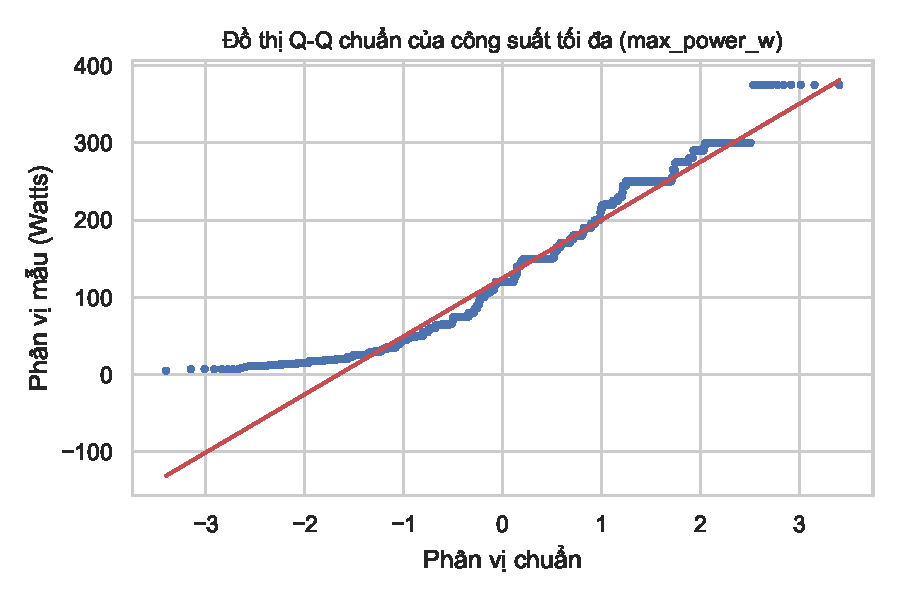
\includegraphics[width=0.64\linewidth]{figures/one_sample_qq.pdf}
  \caption{Đồ thị Q--Q chuẩn của biến công suất tối đa \texttt{max\_power\_w} ($n = 2\,057$).}
  \label{fig:one_sample_qq}
\end{figure}

Tuy nhiên, vì cỡ mẫu rất lớn ($n = 2\,057 \gg 30$), theo Định lý giới hạn trung tâm (CLT)[cite: 7, 16], phân phối của trung bình mẫu $\bar{x}$ vẫn xấp xỉ phân phối chuẩn nên \textbf{kiểm định $t$ một mẫu} hoàn toàn hợp lệ.

\paragraph{Thực hiện kiểm định $t$ một mẫu và ước lượng khoảng tin cậy.}
Thống kê kiểm định $t$ với bậc tự do $\nu = n - 1 = 2\,056$ được tính bằng:
\[
  t_{qs} = \frac{\bar{x} - \mu_0}{SE} = \frac{124{,}93 - 75}{1{,}70} = 29{,}43.
\]
Với mức ý nghĩa $\alpha = 0{,}05$ (một phía phải), giá trị tới hạn là $t_{0{,}95;\ 2\,056} = 1{,}65$, suy ra miền bác bỏ là $RR = (1{,}65;\ +\infty)$. Giá trị quan sát $t_{qs} = 29{,}43$ nằm sâu trong miền bác bỏ với $p = 1{,}71 \cdot 10^{-159} < 0{,}001$, do đó ta bác bỏ giả thuyết $H_0$.

Đồng thời, khoảng tin cậy $95\%$ (hai phía) cho công suất thiết kế tối đa trung bình $\mu$ là:
\[
  CI_{95\%}(\mu) = \bar{x} \pm t_{0{,}975;\ 2\,056} \cdot SE = 124{,}93 \pm 1{,}96 \times 1{,}70 = [121{,}61;\ 128{,}26]\text{\,W}.
\]

\paragraph{Kiểm tra độ bền vững của kết quả.}
Do phân bố của biến \texttt{max\_power\_w} bị lệch phải bởi các dòng card đồ họa cao cấp có mức tiêu thụ lớn (lên tới $375$\,W), nhóm thực hiện thêm hai phép kiểm tra bổ trợ (tổng hợp ở Bảng~\ref{tab:one_sample_summary}) để bảo đảm kết luận không bị chi phối bởi giá trị ngoại lệ hay giả định phân phối chuẩn:
\begin{itemize}\tightlist
  \item \textbf{Kiểm định phi tham số Wilcoxon có dấu :} Phương pháp này kiểm định dựa trên thứ hạng và mức trung vị ($120{,}00$\,W) thay vì trung bình cộng, không yêu cầu giả định phân phối chuẩn và ít chịu ảnh hưởng bởi các điểm ngoại lệ. Với cặp giả thuyết một phía phải so với ngưỡng $75$\,W, kiểm định cho thống kê $W = 1\,553\,910$ và $p = 1{,}60 \cdot 10^{-134} < 0{,}001$, tiếp tục bác bỏ $H_0$.
  \item \textbf{Kiểm định $t$ trên thang đo logarit ($\ln P$):} Việc biến đổi dữ liệu sang thang logarit tự nhiên $\ln(\texttt{max\_power\_w})$ giúp giảm độ lệch phải và đưa phân bố về gần dạng đối xứng hơn. Kiểm định $t$ một mẫu so sánh trung bình của $\ln(\texttt{max\_power\_w})$ với $\ln(75)$ cho $t_{qs} = 15{,}02$ ($\nu = 2\,056$, $p = 8{,}98 \cdot 10^{-49} < 0{,}001$). Khi biến đổi ngược bằng hàm mũ ($e^{\overline{\ln P}}$), trung bình nhân của công suất GPU rời đạt $97{,}34$\,W (khoảng tin cậy $95\%$: $[94{,}08;\ 100{,}71]$\,W), vẫn cao hơn rõ rệt so với mức $75$\,W.
\end{itemize}

\begin{lstlisting}[language=Python]
import numpy as np
import pandas as pd
from scipy import stats

# Doc du lieu va tinh cac dai luong mau
df = pd.read_parquet("data/processed/gpus_analysis.parquet")
power = df["max_power_w"].dropna().astype(float)
n = len(power)
mean_val, sd_val = power.mean(), power.std(ddof=1)
se_val = sd_val / np.sqrt(n)
mu_0 = 75.0

# 1. Kiem tra tinh chuan Shapiro-Wilk
stats.shapiro(power)

# 2. Kiem dinh t mot mau (H1: mu > 75) va KTC 95%
t_stat, p_two = stats.ttest_1samp(power, popmean=mu_0)
p_right = p_two / 2
t_crit = stats.t.ppf(0.975, df=n - 1)
ci_95 = (mean_val - t_crit * se_val, mean_val + t_crit * se_val)

# 3. Kiem tra do ben vung: Wilcoxon va thang logarit
stats.wilcoxon(power - mu_0, alternative="greater")
log_p = np.log(power)
stats.ttest_1samp(log_p, popmean=np.log(mu_0), alternative="greater")
\end{lstlisting}

\begin{table}[H]
  \centering
  \small
  \caption{Tổng hợp kết quả kiểm định trung bình một mẫu cho \texttt{max\_power\_w} (so với ngưỡng $75$\,W).}
  \label{tab:one_sample_summary}
  \renewcommand{\arraystretch}{1.25}
  \resizebox{\linewidth}{!}{%
  \begin{tabular}{|l|l|l|l|l|}
    \hline
    \rowcolor{TableHead}
    \textbf{Phương pháp} & \textbf{Thống kê} & \textbf{Ước lượng} & \textbf{KTC $95\%$} & \textbf{Giá trị $p$} \\ \hline
    Kiểm định $t$ một mẫu (W) & $t_{qs} = 29{,}43$ ($\nu = 2\,056$) & $124{,}93$\,W & $[121{,}61;\ 128{,}26]$\,W & $<$ 0,001 \\ \hline
    Wilcoxon có dấu (W) & $W = 1\,553\,910$ & Trung vị $120{,}00$\,W & -- & $<$ 0,001 \\ \hline
    Kiểm định $t$ trên $\ln P$ & $t_{qs} = 15{,}02$ ($\nu = 2\,056$) & TB nhân $97{,}34$\,W & $[94{,}08;\ 100{,}71]$\,W & $<$ 0,001 \\ \hline
  \end{tabular}%
  }
\end{table}

\subsubsection{Kết luận}

Ở mức ý nghĩa $\alpha = 0{,}05$, có bằng chứng thống kê rất mạnh ($t_{qs} = 29{,}43$, $p < 0{,}001$) khẳng định công suất thiết kế tối đa trung bình của GPU rời lớn hơn đáng kể so với ngưỡng $75$\,W của khe cắm PCIe, với khoảng tin cậy $95\%$ đạt $[121{,}61;\ 128{,}26]$\,W. Kết quả này nhất quán qua cả kiểm định phi tham số Wilcoxon có dấu ($p < 0{,}001$) và kiểm định trên thang đo logarit ($p < 0{,}001$), cho thấy đa số GPU rời cần trang bị đầu cấp nguồn phụ và giải pháp tản nhiệt riêng biệt.


% 5.2 Kiểm định 2 mẫu
\clearpage
\subsection{Bài toán kiểm định hai mẫu độc lập}

\subsubsection{Đề xuất phương pháp}
Card đồ họa rời trên máy tính để bàn (Desktop) và máy tính xách tay (Laptop) chịu các ràng buộc vật lý rất khác nhau về không gian tản nhiệt, kích thước bo mạch và nguồn cấp điện. Trên máy tính để bàn, khe cắm PCIe~x16 cấp tối đa $75$\,W và card có thể nhận thêm công suất từ đầu nguồn phụ của bộ nguồn (PSU), trong khi card đồ họa trên laptop bị giới hạn chặt bởi công suất bộ sạc và khả năng thoát nhiệt của khung máy mỏng.

\textbf{Bài toán.} Với mức ý nghĩa $\alpha = 0{,}05$, công suất thiết kế tối đa trung bình (\texttt{max\_power\_w}) của GPU rời dành cho máy tính để bàn (Desktop) có khác biệt có ý nghĩa thống kê so với GPU rời dành cho máy tính xách tay (Laptop) hay không?

Bài toán sử dụng toàn bộ $2\,057$ card đồ họa rời trong bộ dữ liệu sạch ở Mục~3, chia thành hai nhóm theo biến \texttt{segment}: nhóm Desktop ($n_1 = 1\,786$ card) và nhóm Laptop ($n_2 = 271$ card). Theo Bảng~\ref{tab:two_sample_groups}, công suất trung bình và độ phân tán của nhóm Desktop đều cao hơn rõ rệt so với nhóm Laptop; có tới $71{,}1\%$ card Desktop vượt ngưỡng $75$\,W của khe PCIe, trong khi tỉ lệ này ở Laptop chỉ là $13{,}7\%$.

\begin{table}[H]
  \centering
  \caption{Đặc trưng mẫu của công suất tối đa (W) theo phân khúc thiết bị; $p$ là giá trị $p$ của kiểm định Shapiro--Wilk ở Mục~5.2.2.a.}
  \label{tab:two_sample_groups}
  \resizebox{\linewidth}{!}{%
  \begin{tabular}{lrrrrrrr}
    \toprule
    Phân khúc & Số card & Trung bình & Độ lệch chuẩn & Trung vị & IQR & Min--Max & $p$ \\
    \midrule
    Desktop & $1\,786$ & $137{,}1$ & $74{,}3$ & $140$ & $105$ & $18$--$375$ & $<$ 0,001 \\
    Laptop  & $271$    & $44{,}5$  & $33{,}8$ & $35$  & $30$  & $5$--$220$  & $<$ 0,001 \\
    \bottomrule
  \end{tabular}%
  }
\end{table}

\IfFileExists{generated/two_sample_boxplot.pdf}{%
  \begin{figure}[H]
    \centering
    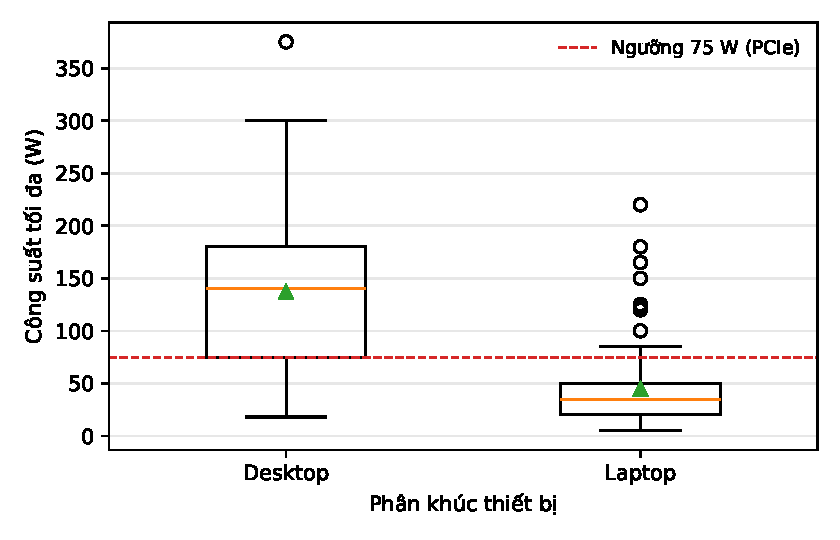
\includegraphics[width=0.72\linewidth]{generated/two_sample_boxplot.pdf}
    \caption{So sánh phân bố công suất tối đa giữa GPU rời Desktop và Laptop. Vạch cam là trung vị, tam giác xanh là trung bình, đường nét đứt đỏ là ngưỡng $75$\,W của khe PCIe.}
    \label{fig:two_sample_boxplot}
  \end{figure}
}{}

Gọi $\mu_1$ và $\mu_2$ lần lượt là công suất tối đa trung bình tổng thể của GPU rời Desktop và Laptop, đặt $\Delta = \mu_1 - \mu_2$. Cặp giả thuyết kiểm định hai phía là
\[
  H_0: \mu_1 = \mu_2 \quad (\Delta = 0), \qquad H_1: \mu_1 \neq \mu_2 \quad (\Delta \neq 0).
\]
Để chọn phép kiểm định phù hợp, ta xét ba điều kiện: tính chuẩn trong từng nhóm, tính đồng nhất phương sai và tính độc lập của các quan sát. Hai điều kiện đầu được kiểm tra ở Mục~5.2.2.a và Mục~5.2.2.b. Điều kiện thứ ba không thỏa mãn tuyệt đối: nhiều mẫu card thương mại dùng chung một kiến trúc chip (cột \texttt{architecture} chỉ có $356$ nhãn khác nhau trên $2\,057$ card, trong đó $222$ ở Desktop và $150$ ở Laptop) nên các quan sát có sự phụ thuộc theo cụm chip. Mục~5.2.2.d kiểm tra thêm độ nhạy bằng cách lấy trung bình theo từng kiến trúc chip để đánh giá ảnh hưởng của hiện tượng này.

\subsubsection{Phân tích kiểm định hai mẫu}

\paragraph{Kiểm tra điều kiện phân phối chuẩn.}
Đặt $H_0$: công suất trong từng nhóm tuân theo phân phối chuẩn; $H_1$: không tuân theo phân phối chuẩn. Kiểm định Shapiro--Wilk bác bỏ $H_0$ ở cả hai nhóm: nhóm Desktop cho $W = 0{,}964$ ($p = 1{,}0 \cdot 10^{-20} < 0{,}001$) và nhóm Laptop cho $W = 0{,}840$ ($p = 4{,}8 \cdot 10^{-16} < 0{,}001$). Nhóm Laptop lệch phải rõ rệt với $34$ quan sát vượt rào chắn trên $Q_3 + 1{,}5\,\text{IQR} = 95$\,W (các dòng GPU hiệu năng cao như GTX~1080 Ti Mobile đạt $220$\,W). Tuy nhiên, vì cỡ mẫu của cả hai nhóm đều lớn ($n_1 = 1\,786$ và $n_2 = 271$), theo định lý giới hạn trung tâm (CLT), phân phối của hiệu hai trung bình mẫu vẫn xấp xỉ chuẩn~\cite{lumley2002}; đồng thời ta đối chiếu thêm bằng kiểm định phi tham số Mann--Whitney~$U$ và kiểm định trên thang logarit.

\IfFileExists{generated/two_sample_qq.pdf}{%
  \begin{figure}[H]
    \centering
    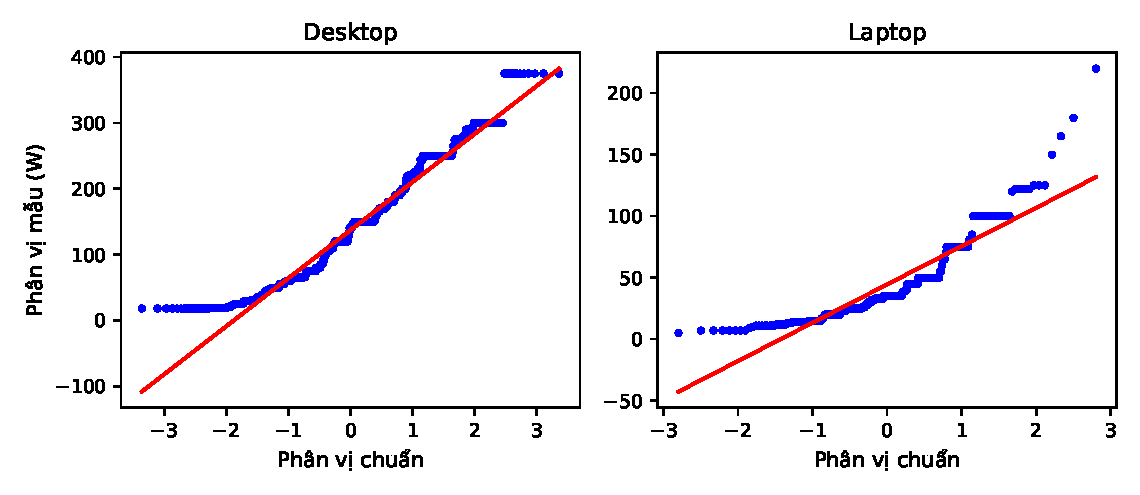
\includegraphics[width=0.88\linewidth]{generated/two_sample_qq.pdf}
    \caption{Đồ thị Q--Q chuẩn của công suất tối đa ở nhóm Desktop và Laptop; đường đỏ là đường tham chiếu phân phối chuẩn.}
    \label{fig:two_sample_qq}
  \end{figure}
}{}

\paragraph{Kiểm định tính đồng nhất phương sai.}
Đặt $H_0: \sigma_1^2 = \sigma_2^2$ và $H_1: \sigma_1^2 \neq \sigma_2^2$. Kiểm định Levene sử dụng trung vị (Brown--Forsythe) cho thống kê $F_{BF} = 197{,}23$ với bậc tự do $(1;\ 2\,055)$ và $p = 7{,}5 \cdot 10^{-43} < 0{,}001$, bác bỏ giả thuyết phương sai bằng nhau. Độ lệch chuẩn của nhóm Desktop ($74{,}3$\,W) gấp $2{,}2$ lần nhóm Laptop ($33{,}8$\,W), đồng thời cỡ mẫu hai nhóm chênh lệch tới $6{,}6$ lần. Do đó, kiểm định $t$ hai mẫu với phương sai gộp không phù hợp và \textbf{kiểm định $t$ Welch} được chọn làm phương pháp suy diễn chính.

\paragraph{Kiểm định Welch hai mẫu độc lập.}
Chênh lệch trung bình mẫu là $\bar{x}_1 - \bar{x}_2 = 137{,}1 - 44{,}5 = 92{,}6$\,W, với sai số chuẩn
\[
  SE_W = \sqrt{\frac{s_1^2}{n_1} + \frac{s_2^2}{n_2}} = 2{,}70\text{\,W}.
\]
Thống kê kiểm định Welch và bậc tự do xấp xỉ Satterthwaite là
\[
  t_W = \frac{\bar{x}_1 - \bar{x}_2}{SE_W} = 34{,}29, \qquad \nu = 749{,}9.
\]
Với mức ý nghĩa $\alpha = 0{,}05$ (hai phía), miền bác bỏ là $|t_W| > t_{0{,}975;\ 749{,}9} = 1{,}96$. Giá trị quan sát $t_W = 34{,}29$ nằm sâu trong miền bác bỏ với $p = 1{,}1 \cdot 10^{-155} < 0{,}001$, nên ta bác bỏ $H_0$. Khoảng tin cậy $95\%$ cho chênh lệch trung bình $\mu_1 - \mu_2$ là
\[
  CI_{95\%}(\Delta) = 92{,}6 \pm 1{,}96 \times 2{,}70 = [87{,}3;\ 97{,}9]\text{\,W}.
\]
Chỉ số độ lớn hiệu ứng Cohen's $d = 1{,}32$ cho thấy mức độ chênh lệch giữa hai phân khúc là rất lớn về mặt thực tiễn. Các lệnh Python thực hiện kiểm định được tóm tắt ở Đoạn code~\ref{lst:two_sample}.

\begin{lstlisting}[caption={Các kiểm định chính của bài toán so sánh hai mẫu (rút gọn từ \texttt{report\_two\_sample.py}).}, label={lst:two_sample}]
import numpy as np
from scipy import stats

desktop = gpu.loc[gpu["segment"] == "Desktop", "max_power_w"]
laptop = gpu.loc[gpu["segment"] == "Laptop", "max_power_w"]

# Normality and equal-variance checks
stats.shapiro(desktop)
stats.shapiro(laptop)
stats.levene(desktop, laptop, center="median")

# Primary Welch t-test and robustness checks
stats.ttest_ind(desktop, laptop, equal_var=False)
stats.ttest_ind(desktop, laptop, equal_var=True)
stats.mannwhitneyu(desktop, laptop, alternative="two-sided")
stats.ttest_ind(np.log(desktop), np.log(laptop), equal_var=False)
\end{lstlisting}

\paragraph{Kiểm tra độ bền vững của kết quả.}
Để bảo đảm kết luận không phụ thuộc vào giả định phân phối hay cấu trúc dữ liệu, ta thực hiện bốn phép kiểm tra bổ trợ (tổng hợp ở Bảng~\ref{tab:two_sample_tests}):
\begin{itemize}
  \item \textbf{Kiểm định $t$ phương sai gộp:} Cho $t = 20{,}22$ ($\nu = 2\,055$, $p = 4{,}9 \cdot 10^{-83} < 0{,}001$), khoảng tin cậy $95\%$ là $[83{,}7;\ 101{,}6]$\,W. Mặc dù $t$ gộp bị kéo giảm vì nhóm lớn hơn (Desktop) lại có phương sai lớn hơn, kết luận bác bỏ $H_0$ vẫn không thay đổi.
  \item \textbf{Kiểm định phi tham số Mann--Whitney $U$:} Không yêu cầu giả định chuẩn, cho $U = 426\,297$ ($p = 3{,}5 \cdot 10^{-91} < 0{,}001$). Xác suất một card Desktop ngẫu nhiên có công suất cao hơn một card Laptop ngẫu nhiên đạt $\hat{P}(X_1 > X_2) = 0{,}881$ ($88{,}1\%$, tương quan nhị phân hạng $r_{rb} = 0{,}762$).
  \item \textbf{Kiểm định Welch trên thang logarit ($\ln P$):} Nhằm giảm ảnh hưởng của độ lệch phải, phép kiểm định cho $t_W = 25{,}43$ ($\nu = 340{,}9$, $p = 1{,}0 \cdot 10^{-80} < 0{,}001$). Biến đổi ngược cho thấy trung bình nhân công suất của Desktop gấp $3{,}32$ lần Laptop (KTC $95\%$: $[3{,}03;\ 3{,}65]$ lần).
  \item \textbf{Kiểm tra mức kiến trúc chip và phân tầng theo hãng:} Khi gộp trung bình công suất theo từng cặp $(\text{phân khúc}, \text{kiến trúc})$ để loại bỏ trùng lặp phiên bản thương mại ($n_1 = 222$, $n_2 = 150$), chênh lệch trung bình vẫn đạt $78{,}3$\,W (KTC $95\%$: $[66{,}5;\ 90{,}1]$\,W; $t_W = 13{,}06$; $p = 1{,}0 \cdot 10^{-31} < 0{,}001$). Khi xét riêng từng hãng sản xuất, chênh lệch Desktop--Laptop vẫn rất lớn ở cả Nvidia ($87{,}9$\,W, $t_W = 24{,}03$) và AMD ($100{,}3$\,W, $t_W = 24{,}18$).
\end{itemize}

\begin{table}[H]
  \centering
  \caption{Tổng hợp kết quả kiểm định hai mẫu và các phép kiểm tra độ bền vững giữa Desktop và Laptop.}
  \label{tab:two_sample_tests}
  \resizebox{\linewidth}{!}{%
  \begin{tabular}{llllll}
    \toprule
    Phương pháp & Thống kê & Ước lượng & KTC $95\%$ & Giá trị $p$ & Kết luận \\
    \midrule
    Welch $t$ (chính, W)          & $t_W = 34{,}29$ ($\nu = 749{,}9$)   & $92{,}6$\,W                        & $[87{,}3;\ 97{,}9]$   & $<$ 0,001 & Bác bỏ $H_0$ \\
    $t$ phương sai gộp (W)        & $t = 20{,}22$ ($\nu = 2\,055$)     & $92{,}6$\,W                        & $[83{,}7;\ 101{,}6]$  & $<$ 0,001 & Bác bỏ $H_0$ \\
    Mann--Whitney $U$             & $U = 426\,297$                     & $\hat{P}(X_1 > X_2) = 0{,}881$     & --                    & $<$ 0,001 & Bác bỏ $H_0$ \\
    Welch $t$ trên $\ln P$        & $t_W = 25{,}43$ ($\nu = 340{,}9$)   & Tỉ số $3{,}32\times$               & $[3{,}03;\ 3{,}65]$   & $<$ 0,001 & Bác bỏ $H_0$ \\
    Welch $t$ mức kiến trúc (W)   & $t_W = 13{,}06$ ($\nu = 330{,}2$)   & $78{,}3$\,W                        & $[66{,}5;\ 90{,}1]$   & $<$ 0,001 & Bác bỏ $H_0$ \\
    \bottomrule
  \end{tabular}%
  }
\end{table}

\subsubsection{Kết luận}
Ở mức ý nghĩa $\alpha = 0{,}05$, có bằng chứng thống kê rất mạnh ($p = 1{,}1 \cdot 10^{-155}$) khẳng định công suất thiết kế tối đa trung bình của GPU rời trên máy tính để bàn cao hơn đáng kể so với GPU rời trên máy tính xách tay. Cụ thể, trong tập dữ liệu khảo sát (giai đoạn 2003--2017), công suất trung bình của GPU Desktop đạt $137{,}1$\,W so với $44{,}5$\,W của GPU Laptop, chênh lệch trung bình $92{,}6$\,W (khoảng tin cậy $95\%$: $[87{,}3;\ 97{,}9]$\,W).

Kết quả này nhất quán qua mọi phương pháp kiểm chứng (Mann--Whitney~$U$, kiểm định trên thang logarit, kiểm định theo kiến trúc chip và phân tầng theo hãng sản xuất) và phản ánh trực tiếp giới hạn tản nhiệt cùng nguồn điện trên thiết bị di động. Tuy nhiên, do nhiều mẫu card thương mại chia sẻ chung một nhân GPU nên các quan sát chưa độc lập hoàn toàn, và kết luận chỉ áp dụng trong phạm vi các GPU rời thuộc cơ sở dữ liệu nghiên cứu.


% 5.3 ANOVA 1 chiều
\clearpage
% Mục 5.1: Bài toán phân tích phương sai ANOVA.
% Số liệu lấy từ generated/anova_*.tex, sinh bởi scripts/reports/report_anova.py.
% Dùng nguyên bộ dữ liệu cuối của Mục 3; mục này không sửa hay tạo thêm dữ liệu.
% Cần: booktabs, graphicx, listings, amsmath; macro \Anova... từ anova_numbers.tex.
% Khi ghép vào báo cáo chính: \setcounter{secnumdepth}{4} và
% \renewcommand{\theparagraph}{\thesubsubsection.\alph{paragraph}} để đánh số 5.1.2.a;
% thêm hai tài liệu lumley2002 và delacre2019 (xem preview_section5_anova.tex).

\subsection{Bài toán phân tích phương sai ANOVA}
\label{sec:anova}

\subsubsection{Đề xuất phương pháp}
\label{sec:anova-method}

Loại bộ nhớ đi theo thế hệ và phân khúc của card: DDR2 có ở các card ra đời 2003--2010,
khoảng \AnovaDdrThreeLaptopPercent\% card DDR3 là card laptop, còn GDDR5X chỉ có ở card cao
cấp ra đời 2016--2017. Vì vậy có thể dùng loại bộ nhớ để chia nhóm khi so sánh công suất.

\begin{center}
\fbox{\parbox{0.92\linewidth}{\textbf{Bài toán.} Với mức ý nghĩa $\alpha = 0{,}05$, công
suất tối đa trung bình (\texttt{max\_power\_w}) có khác nhau giữa các nhóm loại bộ nhớ
(\texttt{memory\_type\_group}) hay không?}}
\end{center}

Bài toán dùng nguyên bộ dữ liệu cuối của Mục~3, gồm \AnovaRows{} card thuộc \AnovaGroups{}
nhóm DDR2, DDR3, GDDR3, GDDR5 và GDDR5X. Nhóm ``Other'' (\AnovaOtherRows{} card) không được
đưa vào so sánh: nhóm này gộp các loại bộ nhớ không liên quan đến nhau (DDR, GDDR2, GDDR4,
HBM), nên trung bình của nó không đại diện cho loại bộ nhớ nào. Theo Bảng~\ref{tab:anova-groups}
và Hình~\ref{fig:anova-box}, công suất trung bình tăng dần từ DDR2 đến GDDR5X, còn độ phân tán
và cỡ nhóm chênh nhau nhiều. Nhóm GDDR5X có \AnovaGddrFiveXCards{} card, chủ yếu là các phiên
bản GTX~1080 và GTX~1080~Ti do nhiều hãng lắp ráp.

\begin{table}[htbp]
  \centering
  \caption{Công suất tối đa (W) theo nhóm loại bộ nhớ; $p$ là kết quả kiểm định
    Shapiro--Wilk ở Mục~\ref{par:anova-normal}}
  \label{tab:anova-groups}
  \begin{tabular}{l r r r r r}
    \toprule
    \textbf{Nhóm} & \textbf{Số card} & \textbf{Trung bình} & \textbf{Độ lệch chuẩn}
      & \textbf{Trung vị} & \textbf{\boldmath$p$} \\
    \midrule
    \csname @@input\endcsname generated/anova_groups.tex
    \bottomrule
  \end{tabular}
\end{table}

\begin{figure}[htbp]
  \centering
  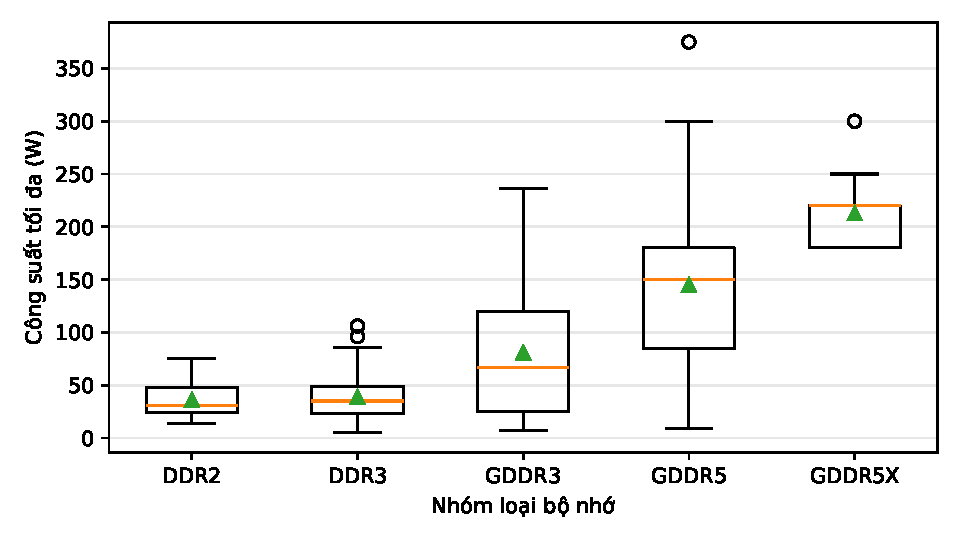
\includegraphics[width=0.75\linewidth]{generated/anova_boxplot.pdf}
  \caption{Công suất tối đa theo nhóm loại bộ nhớ. Vạch cam là trung vị, tam giác là trung
    bình, chấm tròn là giá trị cách tứ phân vị gần nhất quá 1,5 lần khoảng tứ phân vị.}
  \label{fig:anova-box}
\end{figure}

Ta so sánh trung bình của năm nhóm bằng phân tích phương sai (ANOVA) một nhân tố. Gọi
$\mu_1, \dots, \mu_5$ lần lượt là công suất trung bình của các nhóm DDR2, DDR3, GDDR3, GDDR5
và GDDR5X. Cặp giả thuyết là
\[
  H_0: \mu_1 = \mu_2 = \dots = \mu_5, \qquad
  H_1: \text{tồn tại } i \ne j \text{ sao cho } \mu_i \ne \mu_j.
\]

ANOVA một nhân tố cần ba điều kiện: công suất trong mỗi nhóm có phân phối chuẩn, các nhóm có
phương sai bằng nhau, và các quan sát độc lập. Hai điều kiện đầu được kiểm tra ở
Mục~\ref{par:anova-normal} và~\ref{par:anova-levene}. Điều kiện thứ ba không thỏa: nhiều card
là phiên bản của cùng một chip do các hãng khác nhau lắp ráp và thường được ghi cùng một công
suất. Cột \texttt{architecture} chỉ có \AnovaArchLabels{} giá trị khác nhau cho \AnovaRows{}
card; riêng nhóm GDDR5X chỉ có \AnovaGddrFiveXArchLabels. Do đó các giá trị $p$ ở mục này gần
như chắc chắn nhỏ hơn giá trị đúng, các khoảng tin cậy hẹp hơn, và kết quả kiểm định cần được
diễn giải thận trọng. Khác biệt giữa các nhóm trước hết là khác biệt mô tả trong mẫu quan sát.
Đây là hạn chế chính của bài toán.

Hạn chế thứ hai đến từ việc loại dòng khuyết ở Mục~3. Nhóm GDDR3 chỉ còn \AnovaGddrThreeKept{}
trong \AnovaGddrThreeWithPower{} card có ghi công suất, và trung bình của nhóm là
\AnovaGddrThreeMeanKept~W, so với \AnovaGddrThreeMeanAll~W khi tính trên mọi card có ghi công
suất. Các nhóm còn lại gần như không đổi, nên thứ tự giữa các nhóm vẫn giữ nguyên.

\subsubsection{Phân tích ANOVA}

\paragraph{Kiểm tra điều kiện phân phối chuẩn.}
\label{par:anova-normal}
Đặt $H_0$: công suất trong nhóm có phân phối chuẩn; $H_1$: không có phân phối chuẩn.
Shapiro--Wilk bác bỏ $H_0$ ở cả năm nhóm (Bảng~\ref{tab:anova-groups}), nên điều kiện chuẩn
không thỏa. Sai lệch này có thật, không chỉ do kiểm định nhạy khi mẫu lớn: trên đồ thị Q--Q
(Hình~\ref{fig:anova-qq}), các điểm ở hai đầu lệch khỏi đường thẳng, và
\AnovaGddrFiveXLevelCards{} trong \AnovaGddrFiveXCards{} card GDDR5X có công suất đúng bằng một
trong ba mức \AnovaGddrFiveXLevels~W.

Dù vậy vẫn có thể dùng ANOVA, vì thống kê $F$ khá bền với vi phạm giả định chuẩn khi các nhóm
đủ lớn: theo định lý giới hạn trung tâm, trung bình mẫu của mỗi nhóm có phân phối xấp xỉ chuẩn
\cite{lumley2002}. Nhóm nhỏ nhất (\AnovaSizeMinGroup) có \AnovaSizeMin{} card. Với GDDR5X, lập
luận này yếu hơn vì nhóm chỉ gồm vài sản phẩm.

\begin{figure}[htbp]
  \centering
  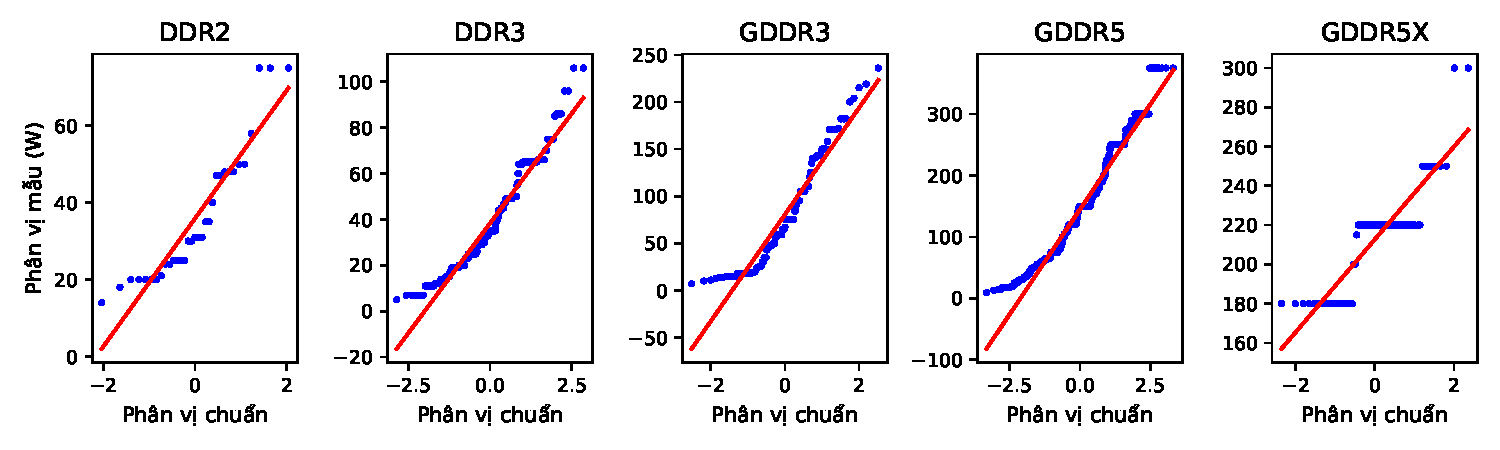
\includegraphics[width=\linewidth]{generated/anova_qq.pdf}
  \caption{Đồ thị Q--Q chuẩn của công suất trong từng nhóm; đường đỏ là đường tham chiếu của
    phân phối chuẩn.}
  \label{fig:anova-qq}
\end{figure}

\paragraph{Kiểm định tính đồng nhất về phương sai.}
\label{par:anova-levene}
Đặt $H_0$: $\sigma_1^2 = \dots = \sigma_5^2$; $H_1$: có ít nhất một phương sai khác. Kiểm
định Levene dùng trung vị (Brown--Forsythe) cho $F_{\mathrm{BF}} = \AnovaLeveneW$ với bậc tự do
$(\AnovaDfBetween;\ \AnovaDfWithin)$, $p < 0{,}001$, nên ta bác bỏ $H_0$. Độ lệch chuẩn của
\AnovaSdMaxGroup{} gấp \AnovaSdRatio{} lần của \AnovaSdMinGroup.

ANOVA cổ điển vẫn là phân tích chính. Nhóm lớn nhất (GDDR5) cũng là nhóm có phương sai lớn
nhất, nên $\mathrm{MSW}$ bị kéo lên và $F$ cổ điển có xu hướng khó bác bỏ $H_0$ hơn.
Mục~\ref{par:anova-check} kiểm tra lại bằng Welch ANOVA và Games--Howell, hai phương pháp không
cần phương sai bằng nhau.

\paragraph{Kiểm định ANOVA.}
\label{par:anova-test}
Từ Bảng~\ref{tab:anova-classic}, thống kê kiểm định và miền bác bỏ là
\[
  F = \frac{\mathrm{MSB}}{\mathrm{MSW}} = \AnovaClassicF, \qquad
  W_\alpha = \bigl(F_{0{,}95;\,\AnovaDfBetween;\,\AnovaDfWithin};\ +\infty\bigr)
    = (\AnovaClassicFCritical;\ +\infty).
\]
Với giả định các quan sát độc lập và phương sai bằng nhau, $F$ thuộc miền bác bỏ và
$p < 0{,}001$, nên ta bác bỏ $H_0$: có ít nhất hai nhóm loại bộ nhớ có công suất trung bình khác
nhau. Hai giả định này không thỏa (Mục~\ref{sec:anova-method} và~\ref{par:anova-levene}), nên
kết luận chịu hạn chế đã nêu.

\begin{table}[htbp]
  \centering
  \caption{Bảng ANOVA một nhân tố cho công suất theo nhóm loại bộ nhớ}
  \label{tab:anova-classic}
  \small
  \begin{tabular}{l r r r r r}
    \toprule
    \textbf{Nguồn biến thiên} & \textbf{\shortstack{Tổng\\bình phương}}
      & \textbf{\shortstack{Bậc\\tự do}} & \textbf{\shortstack{Trung bình\\bình phương}}
      & $F$ & $p$ \\
    \midrule
    Giữa các nhóm & $\mathrm{SSB} = \AnovaSsBetween$ & \AnovaDfBetween
      & $\mathrm{MSB} = \AnovaMsBetween$ & \AnovaClassicF & $<$ 0,001 \\
    Trong các nhóm & $\mathrm{SSW} = \AnovaSsWithin$ & \AnovaDfWithin
      & $\mathrm{MSW} = \AnovaMsWithin$ & & \\
    Tổng & $\mathrm{SST} = \AnovaSsTotal$ & \the\numexpr\AnovaDfBetween+\AnovaDfWithin\relax
      & & & \\
    \bottomrule
  \end{tabular}
\end{table}

Tỉ số $\eta^2 = \mathrm{SSB}/\mathrm{SST} = \AnovaEtaSq$: khác biệt giữa các nhóm chiếm
khoảng \AnovaEtaSqPercent\% tổng biến thiên của công suất. Các lệnh Python dùng trong mục này
được tóm tắt ở Đoạn code~\ref{lst:anova}.

\begin{lstlisting}[language=Python, float=htbp, columns=fixed, label={lst:anova},
  caption={Các kiểm định chính của Mục~\ref{sec:anova} (rút gọn từ \texttt{report\_anova.py})}]
from scipy import stats
from statsmodels.stats.multicomp import pairwise_tukeyhsd
from statsmodels.stats.oneway import anova_oneway

gpu = gpu[gpu["memory_type_group"] != "Other"]
y, g = gpu["max_power_w"], gpu["memory_type_group"]
groups = [y[g == level] for level in g.unique()]
[stats.shapiro(v) for v in groups]      # normality in each group
stats.levene(*groups, center="median")  # equal variances (Brown-Forsythe)
stats.f_oneway(*groups)                 # one-way ANOVA
pairwise_tukeyhsd(y, g.astype(str))     # Tukey HSD
anova_oneway(y, g, use_var="unequal")   # check: Welch ANOVA
stats.kruskal(*groups)                  # check: Kruskal-Wallis
\end{lstlisting}

\paragraph{Kiểm tra sự khác biệt giữa các nhóm.}
\label{par:anova-posthoc}
\begin{table}[!htbp]
  \centering
  \caption{So sánh từng cặp bằng Tukey HSD (chênh lệch = nhóm trước trừ nhóm sau, W)}
  \label{tab:anova-tukey}
  \begin{tabular}{l r c r l}
    \toprule
    \textbf{Cặp} & \textbf{Chênh lệch} & \textbf{KTC 95\%} & \textbf{\boldmath$p$ hiệu chỉnh}
      & \textbf{Kết luận $H_0$} \\
    \midrule
    \csname @@input\endcsname generated/anova_tukey.tex
    \bottomrule
  \end{tabular}
\end{table}
Vì $H_0$ đã bị bác bỏ, ta so sánh $\binom{5}{2} = \AnovaPairs$ cặp nhóm bằng Tukey HSD, có
hiệu chỉnh giá trị $p$ cho việc so sánh nhiều lần. Cỡ nhóm khác nhau nên ta dùng phiên bản
Tukey--Kramer. Với mỗi cặp, $H_0$: $\mu_i = \mu_j$; $H_1$: $\mu_i \ne \mu_j$. Tukey cũng giả định
phương sai bằng nhau, nên với lý do như ở Mục~\ref{par:anova-levene}, phương pháp này khó bác
bỏ $H_0$ hơn ở các cặp gồm những nhóm có phương sai nhỏ.

Theo Bảng~\ref{tab:anova-tukey}, \AnovaPairsSignificant{} trong \AnovaPairs{} cặp có trung
bình khác nhau có ý nghĩa thống kê. Riêng cặp \AnovaPairsNotSignificant{} có khoảng tin cậy
$[\AnovaDdrThreeMinusDdrTwoLow;\ \AnovaDdrThreeMinusDdrTwoHigh]$~W chứa 0, nên chưa đủ bằng
chứng để nói hai nhóm này khác nhau. Khoảng này rộng chủ yếu vì $\mathrm{MSW}$ chung bị phương
sai lớn của GDDR5 kéo lên. Games--Howell dùng phương sai riêng của từng nhóm và cho khoảng hẹp
hơn, $[\AnovaDdrThreeMinusDdrTwoGamesLow;\ \AnovaDdrThreeMinusDdrTwoGamesHigh]$~W, nhưng khoảng
này cũng coi các card là độc lập. Xếp theo công suất trung bình tính trên từng card (dấu
$\approx$ nghĩa là không phát hiện khác biệt):
\[
  \text{DDR2} \approx \text{DDR3} < \text{GDDR3} < \text{GDDR5} < \text{GDDR5X}.
\]

\paragraph{Kiểm tra lại kết luận.}
\label{par:anova-check}
Welch ANOVA không cần phương sai bằng nhau và kiểm soát sai lầm loại I gần mức $\alpha$ khi
phương sai và cỡ nhóm không đều \cite{delacre2019}. Phương pháp này cho $F = \AnovaWelchF$ với
bậc tự do $(\AnovaWelchDfOne;\ \AnovaWelchDfTwo)$, thuộc miền bác bỏ
$(\AnovaWelchFCritical;\ +\infty)$, nên vẫn bác bỏ $H_0$. Games--Howell cũng cho
\AnovaGamesSignificant{} trong \AnovaPairs{} cặp khác nhau, và cặp không khác nhau vẫn là
\AnovaGamesNotSignificant. Kruskal--Wallis, không cần giả định chuẩn, bác bỏ giả thuyết các
nhóm có cùng phân phối ($H = \AnovaKruskalH$, $p < 0{,}001$). Cả ba phương pháp vẫn giả định
các quan sát độc lập, nên không khắc phục được hạn chế ở Mục~\ref{sec:anova-method}.

\subsubsection{Kết luận}

Trong mẫu quan sát, công suất tối đa trung bình khác nhau rõ giữa các nhóm loại bộ nhớ. ANOVA
ở mức ý nghĩa 0,05 bác bỏ giả thuyết các nhóm có cùng trung bình, Welch ANOVA cho cùng kết
luận, và Kruskal--Wallis cho thấy phân phối công suất cũng khác nhau. Vì các quan sát không độc
lập và phương sai không bằng nhau, các kết quả kiểm định này cần được diễn giải thận trọng.
Tính trên từng card, card GDDR5X có công suất trung bình cao hơn card GDDR5 khoảng
\AnovaGddrFiveXMinusGddrFive~W (KTC 95\%:
$[\AnovaGddrFiveXMinusGddrFiveLow;\allowbreak\ \AnovaGddrFiveXMinusGddrFiveHigh]$~W). Khoảng này
coi các card là độc lập nên hẹp hơn thực tế, và con số chủ yếu phản ánh hai dòng GTX~1080 và
GTX~1080~Ti. Giữa DDR2 và DDR3 chưa phát hiện khác biệt.

Kết quả chỉ cho thấy loại bộ nhớ có liên hệ với công suất. Card dùng bộ nhớ đời mới thường
cũng dùng chip mạnh hơn, và card laptop tập trung nhiều ở nhóm DDR3, nên không thể quy hết khác
biệt giữa các nhóm cho loại bộ nhớ; ANOVA một nhân tố chỉ xét một yếu tố nên không tách được
các ảnh hưởng này. Kết luận chỉ áp dụng cho card đồ họa rời (desktop và laptop) trong bộ dữ liệu, chủ yếu
ra đời 2006--2017, và không bao gồm nhóm ``Other''.


% 5.4 ANOVA 2 chiều
\clearpage
% =====================================================================
% Mục 5. Phân tích phương sai hai chiều (Two-Way ANOVA)
%
% Gói cần có trong file chính: amsmath, amssymb, booktabs, tabularx, array,
%   caption, float, graphicx, listings, xcolor.
% Trước khi \input file này, file chính phải nạp các con số do code sinh ra:
%   % Generated by scripts/reports/report_anova_two_way.py; do not edit by hand.
\newcommand{\AnovaAlpha}{0{,}05}
\newcommand{\AnovaTotalCleaned}{2057}
\newcommand{\AnovaAtiDesktop}{77}
\newcommand{\AnovaAtiLaptop}{0}
\newcommand{\AnovaSampleN}{1980}
\newcommand{\AnovaDfErr}{1976}
\newcommand{\AnovaFCrit}{3{,}846}
\newcommand{\AnovaTCrit}{1{,}9612}
\newcommand{\AnovaCellAmdDesktopN}{677}
\newcommand{\AnovaCellAmdLaptopN}{117}
\newcommand{\AnovaCellNvidiaDesktopN}{1032}
\newcommand{\AnovaCellNvidiaLaptopN}{154}
\newcommand{\AnovaRawAmdDesktopMean}{137{,}28}
\newcommand{\AnovaRawAmdLaptopMean}{37{,}03}
\newcommand{\AnovaRawNvidiaDesktopMean}{138{,}06}
\newcommand{\AnovaRawNvidiaLaptopMean}{50{,}18}
\newcommand{\AnovaRawLaptopGapW}{13{,}15}
\newcommand{\AnovaRawAmdDesktopSd}{83{,}76}
\newcommand{\AnovaRawAmdLaptopSd}{28{,}26}
\newcommand{\AnovaRawLeveneW}{76{,}964}
\newcommand{\AnovaRawLeveneP}{$<$ 0{,}001}
\newcommand{\AnovaRawSdRatio}{2{,}96}
\newcommand{\AnovaRawShapiroW}{0{,}9707}
\newcommand{\AnovaRawShapiroP}{$<$ 0{,}001}
\newcommand{\AnovaRawMsErr}{5\,089{,}8}
\newcommand{\AnovaRawFMaker}{2{,}181}
\newcommand{\AnovaRawPMaker}{$=$ 0{,}1399}
\newcommand{\AnovaRawEtaMaker}{0{,}0011}
\newcommand{\AnovaRawFSeg}{397{,}709}
\newcommand{\AnovaRawPSeg}{$<$ 0{,}001}
\newcommand{\AnovaRawEtaSeg}{0{,}1675}
\newcommand{\AnovaRawEtaSegPct}{16{,}8}
\newcommand{\AnovaRawFInter}{1{,}718}
\newcommand{\AnovaRawPInter}{$=$ 0{,}1901}
\newcommand{\AnovaRawEtaInter}{0{,}0009}
\newcommand{\AnovaRawTukeyMinDeskLapW}{87{,}10}
\newcommand{\AnovaRawTukeyMaxDeskLapW}{101{,}04}
\newcommand{\AnovaRawWelchLaptopT}{-3{,}341}
\newcommand{\AnovaRawWelchLaptopP}{$<$ 0{,}001}
\newcommand{\AnovaRawWelchDesktopP}{$=$ 0{,}8401}
\newcommand{\AnovaLogLeveneW}{11{,}558}
\newcommand{\AnovaLogLeveneP}{$<$ 0{,}001}
\newcommand{\AnovaLogSdRatio}{1{,}23}
\newcommand{\AnovaLogShapiroW}{0{,}9622}
\newcommand{\AnovaLogShapiroP}{$<$ 0{,}001}
\newcommand{\AnovaLogAmdLapShapiroW}{0{,}9795}
\newcommand{\AnovaLogAmdLapShapiroP}{$=$ 0{,}0701}
\newcommand{\AnovaLogFMaker}{22{,}537}
\newcommand{\AnovaLogPMaker}{$<$ 0{,}001}
\newcommand{\AnovaLogEtaMaker}{0{,}0113}
\newcommand{\AnovaLogFSeg}{725{,}710}
\newcommand{\AnovaLogPSeg}{$<$ 0{,}001}
\newcommand{\AnovaLogEtaSeg}{0{,}2686}
\newcommand{\AnovaLogEtaSegPct}{26{,}9}
\newcommand{\AnovaLogFInter}{8{,}767}
\newcommand{\AnovaLogPInter}{$=$ 0{,}0031}
\newcommand{\AnovaLogEtaInter}{0{,}0044}
\newcommand{\AnovaGeomAmdDesktop}{108{,}4}
\newcommand{\AnovaGeomNvidiaDesktop}{117{,}5}
\newcommand{\AnovaGeomAmdLaptop}{28{,}2}
\newcommand{\AnovaGeomNvidiaLaptop}{39{,}9}
\newcommand{\AnovaLaptopGeomGapPct}{41{,}5}
\newcommand{\AnovaDesktopGeomGapPct}{8{,}4}
\newcommand{\AnovaLogTukeyDeskP}{$=$ 0{,}0796}
\newcommand{\AnovaLogTukeyLapP}{$<$ 0{,}001}
\newcommand{\AnovaLogMsErr}{0{,}4646}
\newcommand{\AnovaRawLsdSigCount}{4}
\newcommand{\AnovaLogLsdSigCount}{6}
\newcommand{\AnovaLogLsdDeskDiff}{0{,}0805}
\newcommand{\AnovaLogLsdDeskCrit}{0{,}0661}
\newcommand{\AnovaLogLsdLapDiff}{0{,}3474}
\newcommand{\AnovaLogLsdLapCrit}{0{,}1639}
\newcommand{\AnovaLogWelchDesktopP}{$=$ 0{,}0212}
\newcommand{\AnovaLogWelchLaptopP}{$<$ 0{,}001}

% (tạo bằng: python scripts/reports/report_anova_two_way.py).
% Không tham chiếu số mục hay số bảng của mục khác; gọi theo nội dung.
% =====================================================================

\subsection{Phân tích phương sai hai chiều}
\label{sec:anova_two_way}

\subsubsection{Đặt bài toán và giả thuyết kiểm định}

\textbf{Câu hỏi kiểm định:} \emph{Hãng sản xuất (\texttt{manufacturer}: Nvidia và AMD)
cùng phân khúc thiết bị (\texttt{segment}: Desktop và Laptop) có ảnh hưởng đến công suất
thiết kế tối đa của GPU rời hay không, và chênh lệch giữa hai hãng có phụ thuộc vào phân
khúc (hiệu ứng tương tác) hay không?} Với  mức ý nghĩa $\alpha = \AnovaAlpha$.

Theo mô hình ANOVA hai chiều có lặp :
\begin{equation}
  Y_{ijk} = \mu + \tau_i + \beta_j + (\tau\beta)_{ij} + \varepsilon_{ijk},
  \qquad \varepsilon_{ijk} \sim \mathcal{N}(0, \sigma^2)\ \text{độc lập},
  \label{eq:two_way_anova}
\end{equation}
{\sloppy với $i \in \{\text{AMD}, \text{Nvidia}\}$ ($a=2$), $j \in \{\text{Desktop},
\text{Laptop}\}$ ($b=2$), $N = \AnovaSampleN$, $df_E = N - ab = \AnovaDfErr$, cùng ràng buộc
$\sum_i \tau_i = \sum_j \beta_j = \sum_i (\tau\beta)_{ij} = \sum_j (\tau\beta)_{ij} = 0$.

Với cỡ mẫu không cân bằng, ta dùng \textbf{Type III SS} và bác bỏ $H_0$ khi $F >
f_{\alpha;\, df_1;\, df_E}$:\par}
\begin{itemize}\setlength{\itemsep}{1pt}\setlength{\parskip}{0pt}
  \item \textbf{Hãng ($SSG$):} $H_{0a}: \tau_1 = \tau_2 = 0$ đối với $H_{1a}: \exists i,\,
    \tau_i \neq 0$; bác bỏ khi $F_a = \mathrm{MSG}/\mathrm{MSE} >
    f_{\AnovaAlpha;\, 1;\, \AnovaDfErr}$.
  \item \textbf{Phân khúc ($SSB$):} $H_{0b}: \beta_1 = \beta_2 = 0$ đối với $H_{1b}:
    \exists j,\, \beta_j \neq 0$; bác bỏ khi $F_b = \mathrm{MSB}/\mathrm{MSE} >
    f_{\AnovaAlpha;\, 1;\, \AnovaDfErr}$.
  \item \textbf{Tương tác A$\times$B ($SSI$):} $H_{0ab}: (\tau\beta)_{ij} = 0\ \forall i,j$
    đối với $H_{1ab}: \exists (i,j),\, (\tau\beta)_{ij} \neq 0$; bác bỏ khi $F_{ab} =
    \mathrm{MSI}/\mathrm{MSE} > f_{\AnovaAlpha;\, 1;\, \AnovaDfErr}$.
\end{itemize}

\subsubsection{Xử lý dữ liệu}

{\sloppy Từ tập dữ liệu sau tiền xử lý gồm \AnovaTotalCleaned{} GPU rời đầy đủ các biến
bắt buộc, nhóm ATI ghi nhận \AnovaAtiDesktop{} quan sát ở phân khúc Desktop nhưng không
có quan sát nào ở phân khúc Laptop (\AnovaAtiLaptop{} mẫu), làm phát sinh ô khuyết và
không cho phép ước lượng đầy đủ hiệu ứng tương tác. Nhằm bảo đảm tính đầy đủ của mô hình
hai nhân tố $2 \times 2$ với các quan sát lặp tại mọi tổ hợp, phân tích chỉ giữ lại hai
hãng Nvidia và AMD ($N = \AnovaSampleN$, ô có cỡ mẫu nhỏ nhất đạt \AnovaCellAmdLaptopN{}
quan sát). Quy trình thiết lập giả thuyết, chuẩn bị mẫu, kiểm định ANOVA hai chiều và
tổng hợp kết luận được trình bày tại Đoạn code~\ref{lst:anova_call}.\par}

\begin{lstlisting}[language=Python, label={lst:anova_call},
  caption={Truyền dữ liệu đã làm sạch vào hàm chạy ANOVA hai chiều}]
cleaned = preprocess.load_analysis()
hyp = anova.build_gpu_power_hypotheses(alpha=0.05)
sample, col = anova.prepare_two_way_sample(
    cleaned, "max_power_w", "manufacturer", "segment",
    include_a=("Nvidia", "AMD"), log_transform=False,  # True cho thang log
)
res = anova.run_two_way_anova(
    sample, col, "manufacturer", "segment", ss_type="III"
)
conclusions = anova.conclude_two_way_anova(res, hyp)
\end{lstlisting}

\begin{table}[H]
  \centering
  \caption{Thống kê mô tả công suất GPU trên thang gốc (W) và thang logarit ($\ln$W),
    $n = \AnovaSampleN$}
  \label{tab:anova_cells}
  \scriptsize
  \setlength{\tabcolsep}{3pt}
  \begin{tabular}{@{}lrcrrrr@{}}
    \toprule
    \textbf{Tổ hợp} & \textbf{$n$} & \textbf{Gốc: TB $\pm$ SD}
      & \textbf{Trung vị} & \textbf{Log: TB $\pm$ SD}
      & \textbf{TB nhân (W)} & \textbf{Shapiro $W$ ($p$)$^*$} \\
    \midrule
    \csname @@input\endcsname generated/anova_cells_combined.tex
    \bottomrule
    \multicolumn{7}{@{}p{\linewidth}@{}}{\scriptsize $^*$ Kiểm định Shapiro--Wilk theo
      từng ô trên thang log; trên thang gốc cả bốn ô đều cho $p < 0{,}001$.}
  \end{tabular}
\end{table}

\textbf{Nhận xét Bảng~\ref{tab:anova_cells}.} Công suất trung bình của GPU Desktop ở AMD
(\AnovaRawAmdDesktopMean{}~W) và Nvidia (\AnovaRawNvidiaDesktopMean{}~W) vượt trội rõ rệt
so với phân khúc Laptop (\AnovaRawAmdLaptopMean{}~W và \AnovaRawNvidiaLaptopMean{}~W).
Trong phân khúc Desktop, mức công suất trung bình giữa hai hãng gần như tương đương; ngược
lại, ở phân khúc Laptop, Nvidia cao hơn AMD \AnovaRawLaptopGapW{}~W (trung bình nhân
\AnovaGeomNvidiaLaptop{}~W so với \AnovaGeomAmdLaptop{}~W, cao hơn
\AnovaLaptopGeomGapPct{}\%), gợi ý khả năng tồn tại hiệu ứng tương tác giữa hãng và phân
khúc.

\begin{figure}[H]
  \centering
  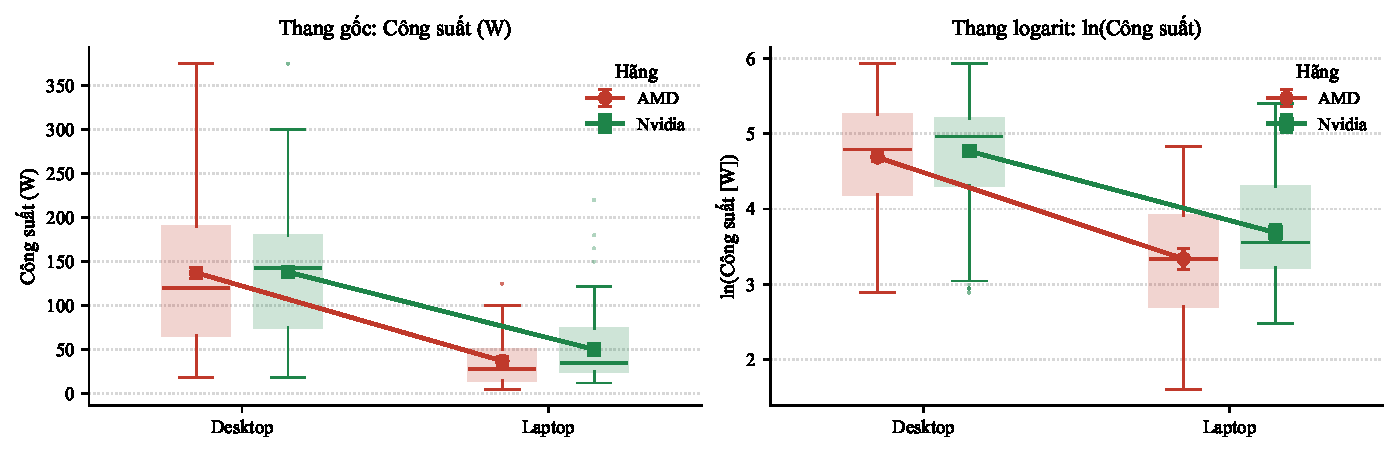
\includegraphics[width=\linewidth]{figures/anova_interaction.pdf}
  \caption{Biểu đồ hộp và đường tương tác trung bình (khoảng tin cậy 95\%) trên thang gốc
    (trái) và thang logarit (phải)}
  \label{fig:anova_interaction}
\end{figure}

\textbf{Nhận xét Hình~\ref{fig:anova_interaction}.} Thang gốc có độ rộng hộp nhóm Desktop
lớn hơn hẳn Laptop và lệch phải mạnh ($\text{SD}_{\max}/\text{SD}_{\min} =
\AnovaRawSdRatio$). Biến đổi logarit làm độ trải bốn nhóm đồng đều hơn rõ rệt và cho thấy
hai đường trung bình không song song (khoảng cách ở Laptop rộng hơn Desktop).

\subsubsection{Kiểm tra giả định và kết quả ANOVA hai chiều}

{\sloppy \textbf{Kiểm tra ba giả định ANOVA.}

\textbf{(1) Tính chuẩn:} trên thang gốc, Shapiro--Wilk bác bỏ ở bốn ô và phần dư
($W = \AnovaRawShapiroW$, $p$~\AnovaRawShapiroP); trên thang log, ô AMD -- Laptop thỏa
chuẩn ($p$~\AnovaLogAmdLapShapiroP), còn phần dư lệch nhẹ do $n$ lớn
($W = \AnovaLogShapiroW$, $p$~\AnovaLogShapiroP) nhưng $n_{ij} \ge
\AnovaCellAmdLaptopN$ bảo đảm kiểm định $F$ bền vững.

\textbf{(2) Đồng nhất phương sai:} Levene thang gốc bác bỏ mạnh
($W = \AnovaRawLeveneW$, $p$~\AnovaRawLeveneP, tỉ số SD $= \AnovaRawSdRatio$); thang log
đưa tỉ số SD còn \textbf{\AnovaLogSdRatio{}} ($< 2{,}0$) và giảm $W$ xuống
$\AnovaLogLeveneW$ ($p$~\AnovaLogLeveneP).

\textbf{(3) Tính độc lập:} các bản ghi ứng với mẫu GPU độc lập, song một số card dùng
chung kiến trúc nên kết quả được kiểm chứng thêm bằng Welch $t$-test.\par}

\begin{table}[H]
  \centering
  \caption{Kết quả ANOVA hai chiều (Type III SS) trên thang gốc và thang logarit
    ($\alpha = \AnovaAlpha$, $f_{\AnovaAlpha;\, 1;\, \AnovaDfErr} = \AnovaFCrit$)}
  \label{tab:anova_table}
  \footnotesize
  \setlength{\tabcolsep}{4pt}
  \begin{tabular}{@{}lrrrrrr@{}}
    \toprule
    \textbf{Nguồn biến thiên} & \textbf{$SS$} & \textbf{$df$} & \textbf{$MS$}
      & \textbf{$F$} & \textbf{$p$-value} & \textbf{$\eta_p^2$} \\
    \midrule
    \csname @@input\endcsname generated/anova_table_combined.tex
    \bottomrule
    \multicolumn{7}{@{}p{\linewidth}@{}}{\scriptsize $^*$ Với Type III SS cho cỡ mẫu không
      cân bằng, tổng $SSG + SSB + SSI + SSE$ nói chung khác $SST$.}
  \end{tabular}
\end{table}

\textbf{Nhận xét Bảng~\ref{tab:anova_table}.}\\
\textbf{-- Trên thang gốc (Panel A):} chỉ có yếu tố \textbf{phân khúc} ảnh hưởng có ý
nghĩa thống kê ($F_b = \AnovaRawFSeg > \AnovaFCrit$, $p$~\AnovaRawPSeg, giải thích
$\eta_p^2 = \AnovaRawEtaSeg$, tương đương \AnovaRawEtaSegPct{}\% phương sai cục bộ),
do đó bác bỏ $H_{0b}$. Ngược lại, yếu tố \textbf{hãng} ($F_a = \AnovaRawFMaker \le
\AnovaFCrit$, $p$~\AnovaRawPMaker) và \textbf{tương tác} ($F_{ab} = \AnovaRawFInter \le
\AnovaFCrit$, $p$~\AnovaRawPInter) đều chưa đủ cơ sở bác bỏ $H_{0a}$ và $H_{0ab}$; nguyên
nhân là độ phân tán công suất trong nhóm Desktop rất lớn làm phương sai sai số
($\mathrm{MSE} = \AnovaRawMsErr$) tăng cao, che lấp khác biệt giữa hai hãng.\\
\textbf{-- Trên thang logarit (Panel B):} sau khi ổn định phương sai
($\mathrm{MSE} = \AnovaLogMsErr$), cả ba thống kê $F$ đều lớn hơn ngưỡng tới hạn
$\AnovaFCrit$ nên bác bỏ đồng thời $H_{0a}$, $H_{0b}$ và $H_{0ab}$. Cụ thể,
\textbf{phân khúc} vẫn là nhân tố chi phối mạnh nhất ($F_b = \AnovaLogFSeg$,
$p$~\AnovaLogPSeg, giải thích \AnovaLogEtaSegPct{}\% phương sai cục bộ), bên cạnh tác
động chính của \textbf{hãng sản xuất} ($F_a = \AnovaLogFMaker$, $p$~\AnovaLogPMaker) và
\textbf{hiệu ứng tương tác có ý nghĩa thống kê} ($F_{ab} = \AnovaLogFInter$,
$p$~\AnovaLogPInter).

\subsubsection{Phân tích Hậu kiểm}

{\sloppy \textbf{(1) Hậu kiểm Fisher's LSD.} Trên thang gốc, Fisher's LSD chỉ phát hiện
\AnovaRawLsdSigCount/6 cặp khác biệt (đều là các cặp giữa Desktop và Laptop; hai hãng
không khác biệt trong từng phân khúc). Trên thang logarit ($\mathrm{MSE} = \AnovaLogMsErr$),
phương pháp này phát hiện cả \AnovaLogLsdSigCount/6 cặp đều khác biệt, gồm cả cặp Laptop
($|\Delta| = \AnovaLogLsdLapDiff > \AnovaLogLsdLapCrit$) và cặp Desktop
($|\Delta| = \AnovaLogLsdDeskDiff > \AnovaLogLsdDeskCrit$). \emph{Lý do cần kiểm chứng
thêm:} Fisher's LSD chỉ giữ mức sai số loại I bằng $\alpha = \AnovaAlpha$ cho từng cặp
riêng lẻ chứ không hiệu chỉnh cho cả họ 6 phép so sánh cùng lúc, nên nguy cơ báo khác biệt
giả (dương tính giả) tăng cao ở những cặp có độ lệch nhỏ như cặp Desktop.\par}

{\sloppy \textbf{(2) Hậu kiểm Tukey HSD.} Để khắc phục hiện tượng phồng sai số loại I khi
so sánh bội của Fisher's LSD, nhóm áp dụng thêm Tukey HSD nhằm kiểm soát sai số loại I
đồng thời trên toàn bộ 6 cặp ở đúng mức $\alpha = \AnovaAlpha$
(Hình~\ref{fig:anova_tukey_ci}).\par}

\begin{figure}[H]
  \centering
  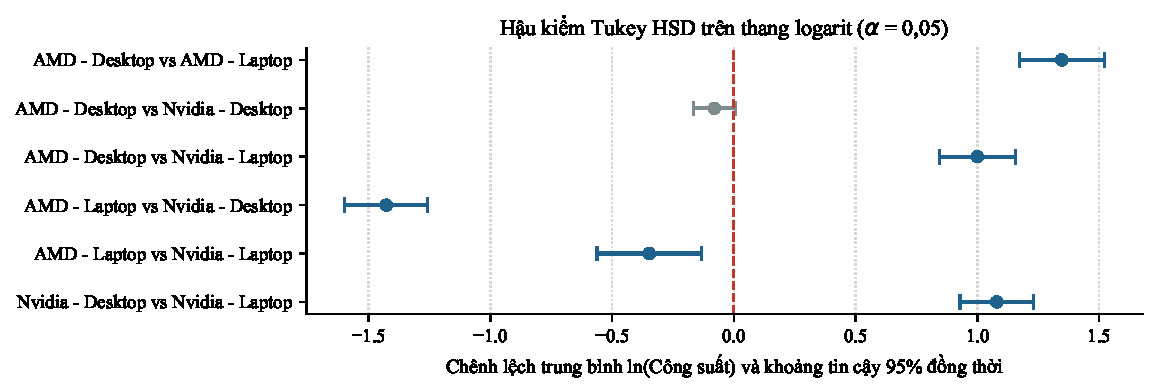
\includegraphics[width=\linewidth]{figures/anova_tukey_ci.pdf}
  \caption{Khoảng tin cậy 95\% đồng thời của hậu kiểm Tukey HSD trên thang logarit}
  \label{fig:anova_tukey_ci}
\end{figure}

\textbf{Nhận xét Hình~\ref{fig:anova_tukey_ci}.} Sau khi hiệu chỉnh bội bằng Tukey HSD
trên thang logarit, có 5/6 cặp sở hữu khoảng tin cậy 95\% đồng thời không chứa 0
($p < 0{,}001$). Riêng cặp AMD -- Desktop so với Nvidia -- Desktop bị cắt qua 0
($p$~\AnovaLogTukeyDeskP), cho thấy chênh lệch rất nhỏ ở phân khúc Desktop mà Fisher's LSD
ghi nhận không còn đủ ý nghĩa thống kê khi kiểm soát sai số toàn họ. Ngược lại, trên
Laptop, Nvidia vẫn cao hơn AMD rõ rệt ($p$~\AnovaLogTukeyLapP), khẳng định trực tiếp nguồn
gốc của hiệu ứng tương tác giữa hãng và phân khúc.

{\sloppy \textbf{(3) Kiểm chứng hiệu ứng đơn bằng Welch $t$-test.} Do mô hình có hiệu ứng
tương tác và kiểm định Levene vẫn ghi nhận khác biệt phương sai giữa các ô, các phương
pháp dùng phương sai gộp ($\mathrm{MSE}$) như ANOVA, Fisher's LSD hay Tukey HSD có thể
bị ảnh hưởng trên thang gốc. Vì vậy, nhóm thực hiện thêm kiểm định hiệu ứng đơn (cố định
từng mức của một nhân tố để so sánh nhân tố còn lại) bằng \textbf{Welch $t$-test} --
phương pháp không đòi hỏi hai nhóm có phương sai bằng nhau
(Bảng~\ref{tab:anova_simple_effects}).\par}

\begin{table}[H]
  \centering
  \caption{Kiểm định hiệu ứng đơn bằng Welch $t$-test (không cần phương sai bằng nhau)}
  \label{tab:anova_simple_effects}
  \footnotesize
  \setlength{\tabcolsep}{3.5pt}
  \begin{tabular}{@{}llrrrrrr@{}}
    \toprule
    & & \multicolumn{3}{c}{\textbf{Thang gốc (W)}}
      & \multicolumn{3}{c}{\textbf{Thang logarit ($\ln$W)}} \\
    \cmidrule(lr){3-5} \cmidrule(lr){6-8}
    \textbf{Điều kiện} & \textbf{Cặp so sánh} & \textbf{Chênh lệch} & \textbf{$t$}
      & \textbf{$p$-value} & \textbf{Chênh lệch} & \textbf{$t$} & \textbf{$p$-value} \\
    \midrule
    \csname @@input\endcsname generated/anova_simple_effects.tex
    \bottomrule
  \end{tabular}
\end{table}

\textbf{Nhận xét Bảng~\ref{tab:anova_simple_effects}.} Kết quả Welch $t$-test nhất quán
trên cả hai thang đo và củng cố trực tiếp kết luận tương tác:\\
\textbf{-- So sánh phân khúc trong từng hãng:} công suất GPU Desktop luôn cao hơn Laptop
rất mạnh ở cả AMD lẫn Nvidia ($p < 0{,}001$).\\
\textbf{-- So sánh hai hãng trong nhóm Laptop:} khi tách riêng phương sai của nhóm Laptop
(không bị độ phân tán lớn của Desktop kéo $\mathrm{MSE}$ lên cao), Nvidia cao hơn AMD rõ
rệt ngay cả trên thang gốc ($t = \AnovaRawWelchLaptopT$, $p$~\AnovaRawWelchLaptopP) lẫn
thang logarit ($p$~\AnovaLogWelchLaptopP), chứng tỏ chênh lệch này là bản chất thật của
dữ liệu chứ không do phép biến đổi logarit tạo ra.\\
\textbf{-- So sánh hai hãng trong nhóm Desktop:} hai hãng gần như tương đương trên thang
gốc ($p$~\AnovaRawWelchDesktopP) và chỉ lệch rất nhẹ trên thang logarit
($p$~\AnovaLogWelchDesktopP, không còn ý nghĩa thống kê sau khi hiệu chỉnh so sánh bội
bằng Tukey HSD).

\subsubsection{Kết luận}

Từ kết quả phân tích phương sai hai chiều ở mức ý nghĩa $\alpha = \AnovaAlpha$, có thể
trả lời trực tiếp câu hỏi kiểm định như sau: Trên thang logarit (thang đo
chính đã ổn định phương sai), dữ liệu có đủ bằng chứng thống kê để bác bỏ đồng thời cả ba giả
thuyết không $H_{0a}$, $H_{0b}$ và $H_{0ab}$. Điều này khẳng định cả \textbf{hãng sản
xuất} ($p$~\AnovaLogPMaker), \textbf{phân khúc thiết bị} ($p$~\AnovaLogPSeg) và
\textbf{hiệu ứng tương tác giữa hai yếu tố} ($p$~\AnovaLogPInter) đều ảnh hưởng có ý
nghĩa đến công suất thiết kế tối đa của GPU rời (trong khi trên thang gốc chỉ bác bỏ được
$H_{0b}$ do phương sai rất lớn ở phân khúc Desktop che lấp khác biệt giữa hai hãng). Cụ thể, kết quả phân tích cho thấy ba điểm chính: 

\textbf{(1) Nhân tố chi phối chính:} phân khúc thiết bị là nguồn biến thiên lớn nhất, giải
thích \AnovaRawEtaSegPct{}\%--\AnovaLogEtaSegPct{}\% phương sai cục bộ, với công suất GPU
Desktop luôn cao hơn vượt trội so với Laptop ở cả hai hãng.

\textbf{(2) Bản chất hiệu ứng tương tác:} chênh lệch giữa hai hãng phụ thuộc rõ rệt vào
phân khúc -- ở phân khúc Desktop, Nvidia và AMD gần như tương đương (trung bình nhân
\AnovaGeomNvidiaDesktop{}~W so với \AnovaGeomAmdDesktop{}~W, không có ý nghĩa theo Tukey
HSD); ngược lại, ở phân khúc Laptop, Nvidia cao hơn AMD \AnovaLaptopGeomGapPct{}\% (trung
bình nhân \AnovaGeomNvidiaLaptop{}~W so với \AnovaGeomAmdLaptop{}~W).

\textbf{(3) Hạn chế và hướng phân tích tiếp theo:} một số mẫu GPU dùng chung kiến trúc
chip (\texttt{architecture}) nên giả định độc lập giữa các quan sát chỉ mang tính gần
đúng, song toàn bộ kết luận chính đều bền vững khi kiểm chứng bằng Welch $t$-test. Đồng
thời, do phần lớn biến thiên công suất vẫn nằm trong nội bộ phân khúc Desktop, mô hình
hồi quy ở mục tiếp theo sẽ bổ sung các biến thông số phần cứng định lượng để giải thích
đầy đủ hơn công suất GPU.


% 5.5 Hồi quy tuyến tính đa biến
\clearpage
% Mục 5.2: Bài toán hồi quy tuyến tính bội.
% Số liệu lấy từ generated/regression_*.tex, sinh bởi scripts/reports/report_regression.py.
% Dùng nguyên bộ dữ liệu cuối của Mục 3 (loại các dòng khuyết xung nhịp lõi);
% mục này không sửa hay tạo thêm dữ liệu.
% Cần: booktabs, graphicx, listings, amsmath; macro \Reg... từ regression_numbers.tex.
% Khi ghép vào báo cáo chính: thêm hai tài liệu cameron2015 và duan1983
% (xem preview_section5_regression.tex).

\subsection{Bài toán hồi quy tuyến tính}
\label{sec:regression}

\subsubsection{Đề xuất phương pháp}
\label{sec:reg-method}

Phân tích phương sai ở Mục~\ref{sec:anova} cho thấy công suất tối đa khác nhau rõ giữa các nhóm
loại bộ nhớ, nhưng chưa tách được tác động riêng của từng thông số phần cứng khi các yếu tố
này cùng thay đổi theo thế hệ sản phẩm. Để định lượng đồng thời mối liên hệ giữa công suất tiêu
thụ tối đa và các đặc trưng kỹ thuật của GPU rời, ta xây dựng mô hình hồi quy tuyến tính bội
trên thang logarit tự nhiên.

\begin{center}
\fbox{\parbox{0.92\linewidth}{\textbf{Bài toán.} Với mức ý nghĩa $\alpha = \RegAlpha$ (độ tin
cậy $\RegConfidence\%$), các thông số kỹ thuật gồm băng thông bộ nhớ, xung nhịp lõi, kích thước
tiến trình chế tạo và dung lượng bộ nhớ có đồng thời liên hệ có ý nghĩa thống kê với công suất
tối đa ($\ln P$) sau khi kiểm soát hãng sản xuất và phân khúc thiết bị hay không?}}
\end{center}

Từ \RegRowsInput{} dòng dữ liệu cuối của Mục~3 (\texttt{gpus\_analysis}), mô hình loại
\RegRowsExcluded{} dòng chỉ bị khuyết xung nhịp lõi (\texttt{core\_speed\_mhz}) và giữ lại
$n = \RegN{}$ quan sát đầy đủ thuộc \RegClusters{} nhãn kiến trúc (\texttt{architecture}) khác
nhau. Biến phụ thuộc là $z_i = \ln P_i$, với $P_i$ là công suất tối đa (\texttt{max\_power\_w},
đơn vị W). Các biến giải thích đưa vào mô hình gồm:
\begin{itemize}
  \item Bốn biến kỹ thuật: $\ln B_i$ với $B_i$ là băng thông bộ nhớ (\texttt{memory\_bandwidth\_gb\_s},
    GB/s); $\ln F_i$ với $F_i$ là xung nhịp lõi (\texttt{core\_speed\_mhz}, MHz); $L_i$ là kích
    thước tiến trình chế tạo (\texttt{process\_nm}, nm); và $\ln M_i$ với $M_i$ là dung lượng
    bộ nhớ quy đổi về GB (\texttt{memory\_mb / 1024}).
  \item Các biến phân loại kiểm soát: hai biến giả hãng sản xuất $D_{i,\mathrm{AMD}}$ và
    $D_{i,\mathrm{ATI}}$ (lấy \texttt{Nvidia} làm nhóm tham chiếu), cùng biến giả phân khúc
    $N_i = 1$ nếu là GPU \texttt{Laptop} và $N_i = 0$ nếu là \texttt{Desktop}.
\end{itemize}

Tương tự hạn chế đã nêu ở Mục~\ref{sec:anova-method}, nhiều card đồ họa trong dữ liệu là các
phiên bản thương mại khác nhau của cùng một kiến trúc chip nên không độc lập hoàn toàn. Do đó,
suy diễn thống kê chính trong mục này sử dụng ma trận hiệp phương sai vững theo cụm
(\textit{cluster-robust}, hiệu chỉnh hữu hạn mẫu CR1) phân nhóm theo \RegClusters{} kiến trúc
\cite{cameron2015}, với bậc tự do phân phối $t$ là $\RegClusters - 1 = \RegPrimaryDfTwo$.

\subsubsection{Mô hình}
\label{sec:reg-model}

Mô hình hồi quy log--tuyến tính bội có dạng:
\begin{equation}
  z_i = \ln P_i = \beta_0 + \beta_1 \ln B_i + \beta_2 \ln F_i + \beta_3 L_i + \beta_4 \ln M_i
        + \gamma_{\mathrm{AMD}} D_{i,\mathrm{AMD}} + \gamma_{\mathrm{ATI}} D_{i,\mathrm{ATI}}
        + \delta N_i + \varepsilon_i.
  \label{eq:reg-model}
\end{equation}

Để kiểm định vai trò đồng thời của bốn thông số kỹ thuật sau khi kiểm soát hãng sản xuất và
loại thiết bị, ta đặt cặp giả thuyết:
\[
  H_0: \beta_1 = \beta_2 = \beta_3 = \beta_4 = 0, \qquad
  H_1: \text{tồn tại ít nhất một } \beta_j \ne 0 \quad (j \in \{1, 2, 3, 4\}).
\]

Kết quả ước lượng bình phương tối thiểu (OLS) kèm ba loại sai số chuẩn (cổ điển OLS, vững
phương sai thay đổi HC3 và vững theo cụm kiến trúc) được trình bày ở Bảng~\ref{tab:reg-coef}.
Thay các hệ số ước lượng vào phương trình~\eqref{eq:reg-model}, ta thu được mô hình thực nghiệm:
\begin{align*}
  \widehat{\ln P_i} ={} & 1{,}173 + 0{,}695 \ln B_i - 0{,}047 \ln F_i + 0{,}018 L_i + 0{,}099 \ln M_i \\
                        & - 0{,}024 D_{i,\mathrm{AMD}} - 0{,}129 D_{i,\mathrm{ATI}} - 0{,}500 N_i.
\end{align*}

\begin{table}[htbp]
  \centering
  \caption{Kết quả ước lượng hồi quy bội cho $\ln P$ ($n = \RegN$, \RegClusters{} cụm kiến trúc)}
  \label{tab:reg-coef}
  \small
  \resizebox{\linewidth}{!}{%
  \begin{tabular}{l r r r r c r}
    \toprule
    \textbf{Biến / Hệ số} & \textbf{Ước lượng} & \textbf{SE (OLS)} & \textbf{SE (HC3)}
      & \textbf{SE (Cụm)} & \textbf{KTC \RegConfidence\% (Cụm)} & \textbf{\boldmath$p$ (Cụm)} \\
    \midrule
    \csname @@input\endcsname generated/regression_coef_table.tex
    \bottomrule
  \end{tabular}%
  }
\end{table}

Mô hình đạt hệ số xác định $R^2 = \RegRSquared$ và $R^2_{\mathrm{adj}} = \RegAdjRSquared$ trên
thang $\ln P$. Kiểm định Wald đồng thời bốn hệ số kỹ thuật theo sai số chuẩn cụm cho
$F(\RegPrimaryDfOne;\ \RegPrimaryDfTwo) = \RegPrimaryF$ với $p = \RegPrimaryP \le \RegAlpha$,
nên ta bác bỏ $H_0$: nhóm thông số kỹ thuật có liên hệ có ý nghĩa thống kê rất mạnh với công
suất GPU.

Bảng~\ref{tab:reg-coef} cũng cho thấy sai số chuẩn cụm lớn gấp khoảng $2$ đến $2{,}5$ lần sai
số chuẩn OLS và HC3, phản ánh rõ sự tương quan giữa các card cùng kiến trúc. Bảng~\ref{tab:reg-effects}
quy đổi từng hệ số sang tác động phần trăm chính xác lên trung bình hình học có điều kiện
$\exp\{\mathrm{E}(\ln P \mid \mathbf{x})\}$ khi giữ các biến còn lại cố định:
\begin{itemize}
  \item \textbf{Băng thông bộ nhớ ($\ln B$):} Là yếu tố chi phối mạnh nhất ($\hat{\beta}_1 = 0{,}695$,
    $p = 7{,}25 \cdot 10^{-83}$). Khi băng thông tăng $1\%$, trung bình hình học công suất tăng
    $100[(1{,}01)^{\hat{\beta}_1} - 1] = 0{,}694\%$.
  \item \textbf{Kích thước tiến trình ($L$):} Có ý nghĩa thống kê cao ($\hat{\beta}_3 = 0{,}018$,
    $p = 2{,}36 \cdot 10^{-10}$). Với cùng băng thông, xung nhịp và dung lượng bộ nhớ, tiến trình
    lớn hơn $1\text{ nm}$ đi kèm công suất cao hơn $100[\exp(\hat{\beta}_3) - 1] = 1{,}840\%$, phản
    ánh hiệu quả năng lượng cải thiện ở các tiến trình thu nhỏ.
  \item \textbf{Dung lượng bộ nhớ ($\ln M$):} Có ý nghĩa thống kê ở mức $\alpha = \RegAlpha$
    ($\hat{\beta}_4 = 0{,}099$, $p = 0{,}0045$); tăng $1\%$ dung lượng VRAM tương ứng mức tăng
    $0{,}098\%$ công suất.
  \item \textbf{Xung nhịp lõi ($\ln F$):} Không có ý nghĩa thống kê ($\hat{\beta}_2 = -0{,}047$,
    $p = 0{,}6628$) sau khi đã kiểm soát băng thông, tiến trình và dung lượng bộ nhớ, do xung nhịp
    cao thường xuất hiện ở các thế hệ chip mới dùng tiến trình nhỏ hơn.
  \item \textbf{Phân khúc thiết bị và hãng sản xuất:} Ở cùng thông số kỹ thuật, GPU
    \texttt{Laptop} có trung bình hình học công suất thấp hơn \texttt{Desktop} là $39{,}333\%$
    ($\hat{\delta} = -0{,}500$, $p = 4{,}20 \cdot 10^{-17}$). Ngược lại, chênh lệch giữa
    \texttt{AMD} ($p = 0{,}4904$) và \texttt{ATI} ($p = 0{,}0296 > \RegAlpha$) so với
    \texttt{Nvidia} đều không đạt mức ý nghĩa $\RegAlpha$ sau khi điều chỉnh thông số kỹ thuật.
\end{itemize}

\begin{table}[htbp]
  \centering
  \caption{Tác động phần trăm chính xác lên trung bình hình học có điều kiện của công suất}
  \label{tab:reg-effects}
  \small
  \begin{tabular}{l r l}
    \toprule
    \textbf{Biến / Hệ số} & \textbf{Tác động (\%)}
      & \textbf{Cơ sở so sánh (giữ các biến khác cố định)} \\
    \midrule
    \csname @@input\endcsname generated/regression_effects_table.tex
    \bottomrule
  \end{tabular}
\end{table}

\subsubsection{Kiểm tra giả định mô hình hồi quy bội}
\label{sec:reg-diagnostics}

Để đánh giá độ tin cậy của mô hình tuyến tính cổ điển và lý giải việc sử dụng sai số chuẩn vững,
ta kiểm tra đa cộng tuyến thông qua hệ số phóng đại phương sai $\mathrm{VIF}_j$
(Bảng~\ref{tab:reg-vif}) cùng các kiểm định giả định trên phần dư OLS (Bảng~\ref{tab:reg-diag}
và Hình~\ref{fig:reg-diag}).

\begin{table}[htbp]
  \centering
  \begin{minipage}[t]{0.40\linewidth}
    \centering
    \caption{Hệ số phóng đại phương sai ($\mathrm{VIF}$)}
    \label{tab:reg-vif}
    \small
    \begin{tabular}{l r}
      \toprule
      \textbf{Biến giải thích} & \textbf{$\mathrm{VIF}_j$} \\
      \midrule
      \csname @@input\endcsname generated/regression_vif_table.tex
      \bottomrule
    \end{tabular}
  \end{minipage}
  \hfill
  \begin{minipage}[t]{0.56\linewidth}
    \centering
    \caption{Các phép kiểm định giả định phần dư OLS}
    \label{tab:reg-diag}
    \small
    \begin{tabular}{l r r}
      \toprule
      \textbf{Phép kiểm định} & \textbf{Thống kê} & \textbf{\boldmath$p$} \\
      \midrule
      \csname @@input\endcsname generated/regression_diagnostics_table.tex
      \bottomrule
    \end{tabular}
  \end{minipage}
\end{table}

\begin{itemize}
  \item \textbf{Đa cộng tuyến:} Giá trị $\mathrm{VIF}$ lớn nhất thuộc về $\ln F$ ($\RegMaxVIF$),
    tiếp theo là $L$ ($3{,}46$) và $\ln M$ ($2{,}85$). Tất cả các biến đều dưới ngưỡng cảnh báo
    $5$, cho thấy mức tương quan giữa các biến giải thích không gây mất ổn định nghiêm trọng
    cho ước lượng hệ số.
  \item \textbf{Tính tuyến tính và phương sai sai số:} Trên biểu đồ \textit{Residuals vs Fitted}
    (Hình~\ref{fig:reg-diag}, góc trên bên trái), đường làm mượt LOWESS bám sát trục $0$, ủng hộ
    dạng hàm tuyến tính trên thang log. Tuy nhiên, biểu đồ \textit{Scale-Location} cùng kiểm
    định Breusch--Pagan ($\mathrm{LM} = 258{,}671$, $p = 3{,}95 \cdot 10^{-52}$) và kiểm định
    White ($\mathrm{LM} = 360{,}689$, $p = 6{,}38 \cdot 10^{-59}$) đều bác bỏ mạnh giả định
    phương sai đồng nhất. Điều này khẳng định việc thay thế sai số chuẩn OLS bằng sai số chuẩn
    vững theo cụm là cần thiết.
  \item \textbf{Phân phối chuẩn và điểm ảnh hưởng:} Kiểm định Shapiro--Wilk bác bỏ phân phối
    chuẩn chính xác của phần dư ($W = 0{,}974$, $p = 1{,}22 \cdot 10^{-17}$), thể hiện qua hai
    đuôi lệch khỏi đường tham chiếu trên đồ thị Q--Q (Hình~\ref{fig:reg-diag}, góc trên bên phải),
    trong khi phần thân trung tâm vẫn bám khá sát đường thẳng. Với cỡ mẫu lớn ($n = \RegN$,
    \RegClusters{} cụm), suy diễn dựa trên phân phối tiệm cận của ước lượng cụm không đòi hỏi
    sai số phải chuẩn tuyệt đối \cite{cameron2015}. Trên đồ thị \textit{Residuals vs Leverage},
    các quan sát vượt đường đồng mức Cook $D = 4/n$ chỉ được dùng để nhận diện các cấu hình đặc
    thù chứ không tự động loại bỏ khỏi dữ liệu.
\end{itemize}

\begin{figure}[htbp]
  \centering
  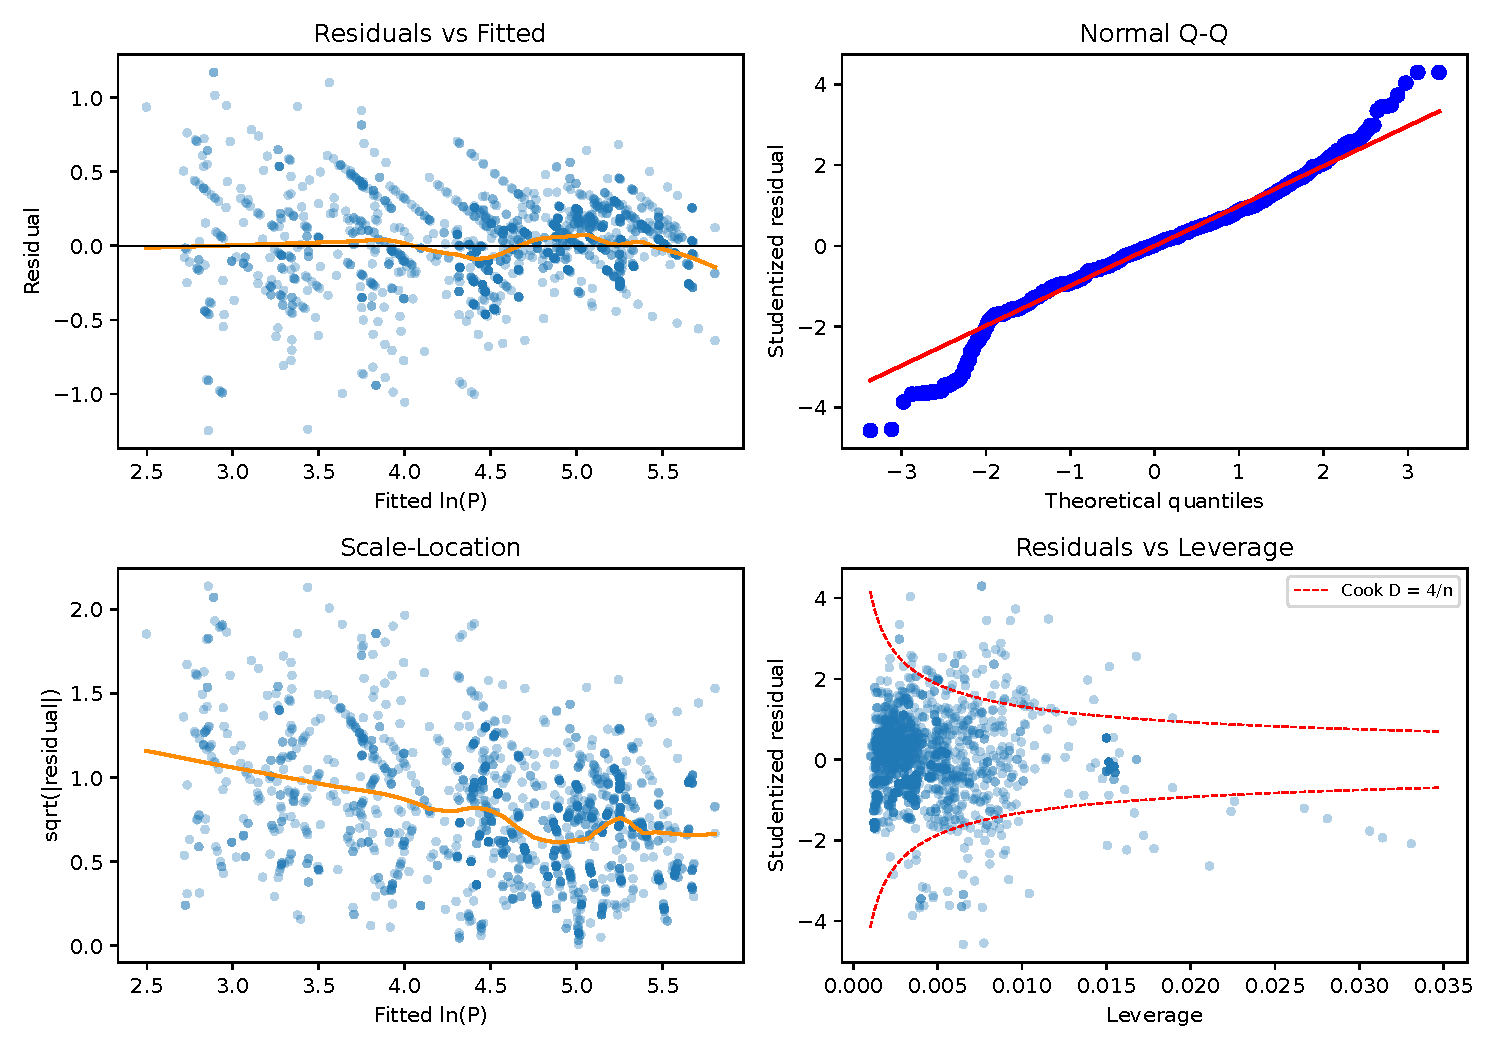
\includegraphics[width=0.92\linewidth]{generated/regression_diagnostics.pdf}
  \caption{Bộ bốn đồ thị chẩn đoán phần dư mô hình hồi quy bội: phần dư theo giá trị khớp,
    đồ thị Q--Q chuẩn, đồ thị Scale-Location và phần dư chuẩn hóa theo đòn bẩy kèm đường đồng
    mức Cook $D = 4/n$.}
  \label{fig:reg-diag}
\end{figure}

Các lệnh Python thực hiện ước lượng vững, kiểm định đồng thời và chẩn đoán mô hình được tóm tắt
ở Đoạn code~\ref{lst:regression}.

\begin{lstlisting}[language=Python, float=htbp, columns=fixed, label={lst:regression},
  caption={Các bước ước lượng và chẩn đoán chính của Mục~\ref{sec:regression} (rút gọn từ \texttt{report\_regression.py})}]
import numpy as np
import statsmodels.api as sm
from scipy import stats
from statsmodels.stats.diagnostic import het_breuschpagan, het_white
from statsmodels.stats.outliers_influence import variance_inflation_factor

ols = sm.OLS(y, X).fit()
hc3 = ols.get_robustcov_results(cov_type="HC3", use_t=True)
clustered = ols.get_robustcov_results(
    cov_type="cluster", groups=arch_groups,
    use_correction=True, df_correction=True, use_t=True,
)
joint_wald = clustered.f_test(restriction_matrix)   # H0: 4 technical slopes = 0
vif = [variance_inflation_factor(X.to_numpy(), i) for i in range(1, X.shape[1])]
bp = het_breuschpagan(ols.resid, X)
white = het_white(ols.resid, X)
shapiro = stats.shapiro(ols.resid)
smearing_factor = np.exp(ols.resid).mean()          # Duan smearing correction
\end{lstlisting}

\subsubsection{Dự báo}
\label{sec:reg-forecast}

Để đánh giá khả năng khái quát hóa trên thang công suất gốc (W) đối với các kiến trúc GPU chưa
từng xuất hiện khi huấn luyện, ta thực hiện kiểm định chéo 5 phần (\textit{5-fold cross-validation})
chia theo từng khối kiến trúc (\texttt{architecture} không trùng lặp giữa tập huấn luyện và tập
kiểm tra). Giá trị dự báo log $\hat{z}_i$ được biến đổi ngược về thang W bằng hệ số hiệu chỉnh
Duan smearing $\hat{\phi} = \frac{1}{n_{\mathrm{train}}}\sum \exp(e_i)$ tính riêng trên từng tập
huấn luyện để tránh rò rỉ dữ liệu \cite{duan1983}:
\[
  \hat{P}_{i,\mathrm{Duan}} = \exp(\hat{z}_i)\,\hat{\phi}.
\]

Kết quả đối chiếu ngoài mẫu trên toàn bộ \RegN{} quan sát (Hình~\ref{fig:reg-cv}) đạt sai số
căn phương trung bình $\mathrm{RMSE} = \RegCVRMSE\text{ W}$, sai số tuyệt đối trung bình
$\mathrm{MAE} = \RegCVMAE\text{ W}$ và hệ số xác định trên thang W là
$R^2_{\mathrm{CV}} = \RegCVRSquaredW$.

\begin{figure}[htbp]
  \centering
  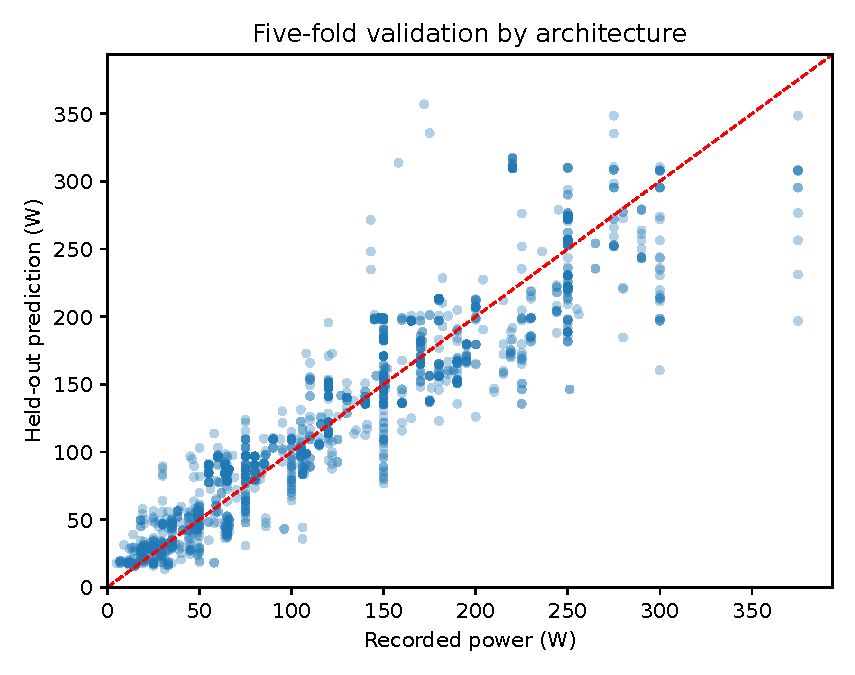
\includegraphics[width=0.68\linewidth]{generated/regression_actual_vs_pred.pdf}
  \caption{Đối chiếu công suất ghi nhận thực tế và công suất dự báo ngoài mẫu (W) từ kiểm định
    chéo 5 phần tách theo kiến trúc; đường đứt nét đỏ là đường lý tưởng $y = x$.}
  \label{fig:reg-cv}
\end{figure}

Bảng~\ref{tab:reg-forecast} minh họa kết quả ước lượng trên ba cấu hình đại diện trong mẫu tại
các mốc tứ phân vị $Q_1, Q_2, Q_3$ của băng thông bộ nhớ:
\begin{itemize}
  \item \texttt{gpu\_id = 1841} (\textit{Radeon HD 6670 MSI Dual Fan 1GB Edition}, ATI, Desktop,
    $B = 64\text{ GB/s}$, $F = 800\text{ MHz}$, $L = 40\text{ nm}$, $M = 1\text{ GB}$, công suất
    ghi nhận $66\text{ W}$);
  \item \texttt{gpu\_id = 3040} (\textit{GeForce GTX 960 MSI OC 2GB Edition}, Nvidia, Desktop,
    $B = 112{,}2\text{ GB/s}$, $F = 1176\text{ MHz}$, $L = 28\text{ nm}$, $M = 2\text{ GB}$, công
    suất ghi nhận $120\text{ W}$);
  \item \texttt{gpu\_id = 1230} (\textit{Radeon RX 480 PowerColor Red Dragon 4GB}, AMD, Desktop,
    $B = 224\text{ GB/s}$, $F = 1120\text{ MHz}$, $L = 14\text{ nm}$, $M = 4\text{ GB}$, công
    suất ghi nhận $120\text{ W}$).
\end{itemize}

\begin{table}[htbp]
  \centering
  \caption{Ước lượng công suất minh họa cho ba cấu hình tiêu biểu trong mẫu}
  \label{tab:reg-forecast}
  \begin{tabular}{r r c r}
    \toprule
    \textbf{\texttt{gpu\_id}} & \textbf{$\widehat{\mathrm{GM}}(P \mid \mathbf{x})$ (W)}
      & \textbf{KTC \RegConfidence\% cho GM (W)} & \textbf{$\hat{P}_{\mathrm{Duan}}$ (W)} \\
    \midrule
    \csname @@input\endcsname generated/regression_forecast_table.tex
    \bottomrule
  \end{tabular}
\end{table}

Cần lưu ý ba giới hạn khi sử dụng các con số ở Bảng~\ref{tab:reg-forecast}: thứ nhất, khoảng tin
cậy $\RegConfidence\%$ trong bảng bao phủ \emph{trung bình hình học có điều kiện}
$\widehat{\mathrm{GM}}(P \mid \mathbf{x}) = \exp(\mathbf{x}^\top \hat{\boldsymbol{\theta}})$
tính theo ma trận hiệp phương sai cụm, không phải khoảng dự báo cho một sản phẩm mới đơn lẻ;
thứ hai, do phương sai sai số thay đổi theo cấu hình, một hệ số hiệu chỉnh Duan tổng quát
$\hat{\phi}$ không bảo đảm ước lượng không chệch cho trung bình số học có điều kiện tại mọi
điểm; thứ ba, mô hình chỉ áp dụng trong miền thông số của bộ dữ liệu (card rời giai đoạn
2006--2017) và không nên ngoại suy cho các thế hệ GPU hiện đại ngoài miền quan sát.

\subsubsection{Kết luận}
\label{sec:reg-conclusion}

Mô hình hồi quy log--tuyến tính bội giải thích được $87{,}95\%$ biến thiên của $\ln P$ trong mẫu
($R^2 = \RegRSquared$) và $83{,}64\%$ biến thiên công suất trên thang W khi kiểm định chéo tách
theo kiến trúc ($R^2_{\mathrm{CV}} = \RegCVRSquaredW$, $\mathrm{RMSE} = \RegCVRMSE\text{ W}$).
Tại mức ý nghĩa $\alpha = \RegAlpha$ với sai số chuẩn cụm theo \RegClusters{} kiến trúc, băng
thông bộ nhớ là yếu tố giải thích mạnh nhất, tiếp theo là phân khúc thiết bị (Laptop thấp hơn
Desktop gần $40\%$ về trung bình hình học ở cùng thông số), kích thước tiến trình bán dẫn và dung
lượng VRAM; trong khi xung nhịp lõi và thương hiệu hãng sản xuất không tạo ra khác biệt có ý
nghĩa thống kê sau khi đã kiểm soát các đặc trưng phần cứng còn lại.

% Mục 6 & Mục 7 (giữ nguyên khung để hoàn thiện sau)
\clearpage
\section{Thảo luận và mở rộng}
[Tóm tắt phát hiện chính, giới hạn và hướng nghiên cứu tiếp theo.]

\section{Nguồn dữ liệu và nguồn code}
\begin{itemize}
  \item Dữ liệu: [Tên nguồn và đường dẫn].
  \item Mã nguồn: [Đường dẫn kho mã hoặc tệp đính kèm].
\end{itemize}

% ==================== TAI LIEU THAM KHAO ==========================
\clearpage
\renewcommand{\refname}{Tài liệu tham khảo}
\begin{thebibliography}{99}
  % Các tài liệu đã có từ Mục 3 và Mục 5
  \bibitem{vandenbroeck2005} J.~Van den Broeck, S.~Argeseanu Cunningham, R.~Eeckels, and
    K.~Herbst, ``Data cleaning: Detecting, diagnosing, and editing data abnormalities,''
    \emph{PLoS Med.}, vol.~2, no.~10, p.~e267, 2005, doi: 10.1371/journal.pmed.0020267.
  \bibitem{donders2006} A.~R.~T. Donders, G.~J.~M.~G. van der Heijden, T.~Stijnen, and
    K.~G.~M. Moons, ``Review: A gentle introduction to imputation of missing values,''
    \emph{J. Clin. Epidemiol.}, vol.~59, no.~10, pp.~1087--1091, 2006,
    doi: 10.1016/j.jclinepi.2006.01.014.
  \bibitem{lumley2002} T.~Lumley, P.~Diehr, S.~Emerson, and L.~Chen, ``The importance of
    the normality assumption in large public health data sets,'' \emph{Annu. Rev. Public
    Health}, vol.~23, pp.~151--169, 2002, doi: 10.1146/annurev.publhealth.23.100901.140546.
  \bibitem{delacre2019} M.~Delacre, C.~Leys, Y.~L. Mora, and D.~Lakens, ``Taking parametric
    assumptions seriously: Arguments for the use of Welch's $F$-test instead of the classical
    $F$-test in one-way ANOVA,'' \emph{Int. Rev. Soc. Psychol.}, vol.~32, no.~1, p.~13, 2019,
    doi: 10.5334/irsp.198.
  \bibitem{cameron2015} A.~C. Cameron and D.~L. Miller, ``A practitioner's guide to
    cluster-robust inference,'' \emph{J. Human Resources}, vol.~50, no.~2, pp.~317--372,
    2015, doi: 10.3368/jhr.50.2.317.
  \bibitem{duan1983} N.~Duan, ``Smearing estimate: A nonparametric retransformation
    method,'' \emph{J. Amer. Statist. Assoc.}, vol.~78, no.~383, pp.~605--610, 1983,
    doi: 10.1080/01621459.1983.10478017.

  % Tài liệu giữ chỗ (placeholder) cho các trích dẫn ref1..ref19 ở Mục 2
  \bibitem{ref1} [Chờ bổ sung tài liệu tham khảo \texttt{ref1} cho Mục 2 (ngưỡng 75 W khe PCIe).]
  \bibitem{ref2} [Chờ bổ sung tài liệu tham khảo \texttt{ref2} cho Mục 2.]
  \bibitem{ref3} [Chờ bổ sung tài liệu tham khảo \texttt{ref3} cho Mục 2.]
  \bibitem{ref4} [Chờ bổ sung tài liệu tham khảo \texttt{ref4} cho Mục 2.]
  \bibitem{ref5} [Chờ bổ sung tài liệu tham khảo \texttt{ref5} cho Mục 2.]
  \bibitem{ref6} [Chờ bổ sung tài liệu tham khảo \texttt{ref6} cho Mục 2.]
  \bibitem{ref7} [Chờ bổ sung tài liệu tham khảo \texttt{ref7} cho Mục 2.]
  \bibitem{ref8} [Chờ bổ sung tài liệu tham khảo \texttt{ref8} cho Mục 2.]
  \bibitem{ref9} [Chờ bổ sung tài liệu tham khảo \texttt{ref9} cho Mục 2.]
  \bibitem{ref10} [Chờ bổ sung tài liệu tham khảo \texttt{ref10} cho Mục 2.]
  \bibitem{ref11} [Chờ bổ sung tài liệu tham khảo \texttt{ref11} cho Mục 2.]
  \bibitem{ref12} [Chờ bổ sung tài liệu tham khảo \texttt{ref12} cho Mục 2.]
  \bibitem{ref13} [Chờ bổ sung tài liệu tham khảo \texttt{ref13} cho Mục 2.]
  \bibitem{ref14} [Chờ bổ sung tài liệu tham khảo \texttt{ref14} cho Mục 2.]
  \bibitem{ref15} [Chờ bổ sung tài liệu tham khảo \texttt{ref15} cho Mục 2.]
  \bibitem{ref16} [Chờ bổ sung tài liệu tham khảo \texttt{ref16} cho Mục 2.]
  \bibitem{ref17} [Chờ bổ sung tài liệu tham khảo \texttt{ref17} cho Mục 2.]
  \bibitem{ref18} [Chờ bổ sung tài liệu tham khảo \texttt{ref18} cho Mục 2.]
  \bibitem{ref19} [Chờ bổ sung tài liệu tham khảo \texttt{ref19} cho Mục 2.]
\end{thebibliography}

% ==================== PHU LUC ====================================
\clearpage
\appendix
\phantomsection
\section*{Phụ lục A}
\addcontentsline{toc}{section}{Phụ lục A}
\phantomsection
\subsection*{Đoạn code được sử dụng}
\addcontentsline{toc}{subsection}{Đoạn code được sử dụng}
[Dán mã nguồn đầy đủ vào môi trường lstlisting, hoặc dùng lệnh dưới đây.]

% Neu co tep phan_tich.py, bo dau % o dong sau:
% \lstinputlisting[language=Python]{phan_tich.py}

\end{document}
